\chapter[Dinâmica dos fluidos computacional]{Dinâmica dos fluidos computacional}
\label{capitulo:Cap2}

O escoamento isotérmico de um fluido newtoniano é descrito pelas equações advindas da conservação da quantidade de movimento, ou de Navier-Stokes, e da conservação de massa. Nos casos em que ocorram variações significativas de temperatura ou em escoamentos compressíveis, a equação da conservação da energia deve ser incorporada ao sistema. Essas equações, em conjunto com a relação constitutiva, formam um sistema de equações diferenciais não lineares que descrevem o comportamento do escoamento no tempo e no espaço. 

Neste trabalho, são investigados escoamentos incompressíveis, isotérmicos e com contornos móveis. As seções seguintes apresentam a abordagem adotada para a resolução desse tipo de problema, bem como sua implementação computacional. Adota-se uma descrição Euleriana-Lagrangiana Arbitrária (ALE) para representar as equações, e a discretização espacial é realizada por meio do método dos elementos finitos (FEM) ou da análise isogeométrica (AIG).

Para tratar questões numéricas recorrentes nesse tipo de equações, como as oscilações espúrias em casos de convecção dominante, típicas da aplicação direta do método dos resíduos ponderados na formulação clássica de Galerkin, emprega-se a metodologia Streamline Upwind/Petrov-Galerkin (SUPG). Além disso, a estabilização Pressure-Stabilizing/Petrov-Galerkin (PSPG) é aplicada com o objetivo de contornar as condições de \textit{Ladyzhenskaya–Babuška–Brezzi} (LBB) associadas aos escoamentos incompressíveis, permitindo o uso estável de um mesmo espaço de funções de aproximação para pressão e velocidade. A integração temporal é realizada por meio do método $\alpha$-generalizado.

Ao final deste capítulo, apresenta-se um algoritmo que descreve o esquema de solução computacional adotado neste trabalhos para a mecânica dos fluidos, seguido da simulação de casos clássicos para a verificação da metodologia proposta.

\section{Equações governantes na descrição Euleriana} 

\subsection{Equação da conservação da massa}

Para obter a equação da conservação da massa na descrição espacial, considera-se um volume de controle infinitesimal fixo no espaço, permeável à matéria e submetido a um escoamento com velocidade $\velocity$, cujos componentes são $u_1$, $u_2$ e $u_3$ (conforme a \autoref{fig:volInf_fluxoMassa}). Para um intervalo de tempo infinitesimal $\deriv t$, a lei da conservação da massa estabelece que a variação de massa dentro do volume de controle deve ser igual ao balanço do fluxo líquido de massa que atravessa suas fronteiras, podendo ser expressa matematicamente da seguinte forma:

\begin{align}
	\begin{split}
	\frac{\partial \density}{\partial t}\deriv V =& \left(\density u_1 \deriv A_{1}  +  \density u_2 \deriv A_{2} + \density u_3  \deriv A_{3} \right) - \\  &\left(\left(\density u_1 + \frac{\partial \density u_1}{\partial y_1}\deriv y_1 \right)\deriv A_{1} + \left(\density u_2+ \frac{\partial \density u_2}{\partial y_2}\deriv y_2 \right) \deriv A_{2} + \left(\density u_3 + \frac{\partial \density u_3}{\partial y_3}\deriv y_3 \right) \deriv A_{3}\right), \label{eq:conser_massa_0} 
	\end{split}
\end{align}

\noindent com $\density$ sendo a densidade de massa do fluido e $\deriv A_{i}$ a área referente à face ortogonal ao eixo $y_i$. Considerando que $\deriv V = \deriv y_1 \deriv y_2 \deriv y_3 = \deriv y_1 \deriv A_1 = \deriv y_2 \deriv A_2 = \deriv y_3 \deriv A_3 $  e manipulando-se algebricamente a Equação \eqref{eq:conser_massa_0}, resulta:

\begin{align}
	\frac{\partial \density}{\partial t} = - \frac{\partial \density u_{1}}{\partial y_1} - \frac{\partial \density u_{2}}{\partial y_2}- \frac{\partial \density u_{3}}{\partial y_3}.
\end{align}

\begin{figure}[!htbp]
	\caption{Volume de controle infinitesimal: Fluxo de massa}
	\begin{center}
		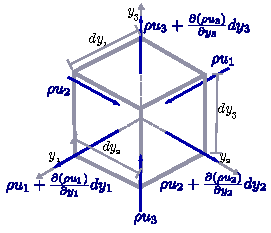
\includegraphics[scale=1.5,trim=0cm 0.0cm 0cm 0.0cm, clip=true]{Imagens/Cap2/volInf_fluxoMassa.pdf}	
	\end{center}
	\legend{Fonte: Elaborada pela autora}
	\label{fig:volInf_fluxoMassa}
\end{figure}

Para escoamentos incompressíveis, quando $\density$ é constante ao longo do tempo, a equação fica reduzida a:

\begin{align}
	 \frac{\partial u_{1}}{\partial y_1} + \frac{\partial u_{2}}{\partial y_2} + \frac{\partial u_{3}}{\partial y_3} = 0, 
\end{align} 

\noindent ou ainda:

\begin{align}
	\divergence \cdot \velocity = 0.
	\label{eq:conser_massa_incom} 
\end{align} 

\noindent onde $\divergence \cdot (\velocity)$ é o divergente de $\velocity$ em relação às coordenadas Eulerianas $\ePosition$.

\subsection{Equação da quantidade de movimento}

Para um volume de controle infinitesimal, a lei da conservação da quantidade de movimento afirma que a variação temporal da quantidade de movimento no interior do volume é determinada pela diferença entre o fluxo de quantidade de movimento que entra e o que sai pelas suas fronteiras, somada à resultante das forças aplicadas sobre o volume de controle.

Para chegar-se à equação da quantidade de movimento em sua forma conservativa e seguindo a descrição espacial, inicia-se com a avaliação das forças que atuam sobre um volume de controle infinitesimal no instante atual, como ilustrado na \autoref{fig:volInf_tensao}, onde são mostradas apenas as componentes que atuam na direção $y_1$. Somando-se vetorialmente as componentes de forças externas e internas na direção $y_1$, chega-se na seguinte relação:

\begin{align}
	\begin{split}
	F_1 =& -\left(\stress_{11}\deriv y_2 \deriv y_3 + \stress_{12}\deriv y_1 \deriv y_3 + \stress_{13}\deriv y_1 \deriv y_2\right) + \\ & \left(\left(\stress_{11} + \frac{\partial \stress_{11}}{\partial y_1}\deriv y_1 \right)\deriv y_2 \deriv y_3 + \left(\stress_{12}+ \frac{\partial \stress_{12}}{\partial y_2}\deriv y_2\right)\deriv y_1 \deriv y_3 + \left(\stress_{13}+ \frac{\partial \stress_{13}}{\partial y_3}\deriv y_3\right)\deriv y_1 \deriv y_2\right) + \\& b_{1}\deriv y_1 \deriv y_2 \deriv y_3, \label{eq:equil_forca_y1} 
	\end{split}
\end{align}	

\noindent onde $F_1$ representa a resultante das forças externas na direção $y_1$; $\stress_{ij}$ são as componentes $ij$ do tensor das tensões de Cauchy ($\stressTensor$); e $b_1$ representa a componente do vetor força de campo por unidade de volume na direção $y_1$. Dividindo-se Equação \eqref{eq:equil_forca_y1} por $\deriv V$ e efetuando as subtrações, tem-se a componente de força resultante por unidade de volume na direção de $y_1$ ($q_1$):

\begin{align}
		q_1 =\frac{\partial \stress_{11}}{\partial y_1} + \frac{\partial \stress_{12}}{\partial y_2} + \frac{\partial \stress_{13}}{\partial y_3} + b_{1}.
\end{align}	

\begin{figure}[!htbp]
	\caption{Volume de controle infinitesimal: Componentes de força na direção $y_1$}
	\begin{center} 
	%\vspace{-1em} % Diminui o espaço antes da figura
	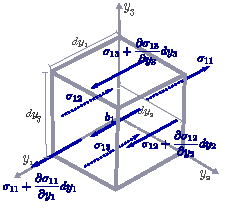
\includegraphics[scale=1.5,trim=0cm 0.0cm 0cm 0.0cm, clip=true]{Imagens/Cap2/volInf_tensao.pdf}	
	\label{fig:volInf_tensao}
	\end{center}
	\legend{Fonte: Elaborada pela autora}
\end{figure}

Seguindo a mesma ideia para as direções $y_2$ e $y_3$, escreve-se:

\begin{align}
	q_2 =\frac{\partial \stress_{21}}{\partial y_1} + \frac{\partial \stress_{22}}{\partial y_2} + \frac{\partial \stress_{23}}{\partial y_3} + b_{2},
\end{align}	

\noindent e

\begin{align}
	q_3 =\frac{\partial \stress_{31}}{\partial y_1} + \frac{\partial \stress_{32}}{\partial y_2} + \frac{\partial \stress_{33}}{\partial y_3} + b_{3},
\end{align}

\noindent ou ainda, de forma simbólica:

\begin{align}
	\mathbf{q} = \divergence \cdot \stressTensor + \mathbf{b}.
\end{align}

Realizando-se o balanço da quantidade de movimento no volume de controle infinitesimal da \autoref{fig:volInf_consQtdeMov}, e aplicando-se o princípio da conservação da quantidade de movimento, pode-se escrever:

\begin{align}
	\begin{split}
	\frac{\partial \density \velocity}{\partial t}\deriv V =& u_1\density \velocity \deriv A_1 + u_2\density \velocity \deriv A_2 + u_3 \density \velocity \deriv A_3 - \\
	 & \left(\left(u_1 \density \velocity + \frac{\partial u_1 \density \velocity}{\partial y_1}\deriv y_1 \right)\deriv A_1 + \left(u_2 \density \velocity + \frac{\partial u_2 \density \velocity}{\partial y_2}\deriv y_2 \right)\deriv A_2 \right. + \\ & \left.   \left(u_3 \density \velocity + \frac{\partial u_3 \density \velocity}{\partial y_3}\deriv y_3 \right)\deriv A_3\right) + \mathbf{q} \deriv V,
	\label{eq:QM_0} 
	\end{split}
\end{align}	

\noindent dividindo-se a Equação \eqref{eq:QM_0} por $\deriv V$ e efetuando-se as subtrações, chega-se a:

\begin{align}
		\frac{\partial \density \velocity}{\partial t} = 
		-\frac{\partial u_1 \density \velocity}{\partial y_1} 
		-\frac{\partial u_2 \density \velocity}{\partial y_2}  
		-\frac{\partial u_3 \density \velocity}{\partial y_3} + \mathbf{q},
		\label{eq:QM_1} 
\end{align}

\noindent ou ainda, considerando que $\density$ é constante:

\begin{align}
	\density\left(\frac{\partial\velocity}{\partial t} + \divergence \cdot \left(\velocity\otimes\velocity\right) - \sbodyforce \right) - \divergence \cdot \stressTensor  &= \vzero, \label{eq:QM_2} 
\end{align}

\noindent onde $\sbodyforce = \mathbf{b}/\density$ representa a força de campo por unidade de massa.

\begin{figure}[!htbp]
	\caption{Volume de controle infinitesimal: Fluxo de quantidade de Movimento}
	\begin{center}
	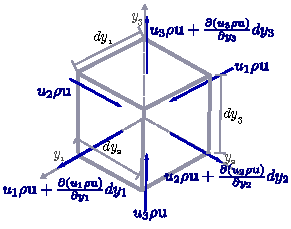
\includegraphics[scale=1.5,trim=0cm 0.0cm 0cm 0.0cm, clip=true]{Imagens/Cap2/volInf_consQtdeMov.pdf}	
	\end{center}
	\legend{Fonte: Elaborada pela autora}
	\label{fig:volInf_consQtdeMov}
\end{figure}

Da consideração da equação da continuidade, a Equação \eqref{eq:QM_2} pode ser rescrita ainda em sua forma convectiva como:

\begin{align}
	\density\left(\frac{\partial\velocity}{\partial t} + \left( \velocity \cdot \gradient \right)  \velocity  - \sbodyforce \right) - \divergence \cdot \stressTensor = \vzero. \label{eq:Navier-Stokes} 
\end{align}

\subsection{Relação constitutiva}

O tensor de tensões de Cauchy $\stressTensor$ é definido para fluidos newtonianos incompressíveis pela seguinte relação constitutiva:

\begin{align}
\stressTensor &= -\press \unittensor + 2\viscosity\straintensor(\velocity),\label{eq:tensor_tensoes_fluido}
\end{align}

\noindent onde $\press$ representa a pressão, $\viscosity$ a viscosidade dinâmica do fluido e $\straintensor(\bullet)$ é o tensor taxa de deformação Euleriana, definido como:

\begin{align}
\straintensor(\bullet) = \frac{1}{2}\left(\gradient (\bullet) + \gradient (\bullet)^{T}\right). 
\label{eq:tensor_taxa_defor}
\end{align}


\section{Descrição Euleriana-Lagrangiana arbitrária (ALE)} \label{capitulo:Cap2:ALE}

A descrição Lagrangiana-Euleriana arbitrária \cite{DoneaGH:1982,HughesLZ:1981} representa uma generalização das descrições puramente Lagrangiana e puramente Euleriana do movimento do contínuo. A descrição Lagrangiana fixa a atenção em pontos materiais do contínuo, enquanto que, na descrição Euleriana, considera-se uma porção fixa do espaço ocupada pelo contínuo e analisam-se os pontos materiais que passam por essa porção ao longo do tempo. Como consequência, na descrição puramente Lagrangiana a malha computacional move-se com o contínuo, enquanto que, na Euleriana, a malha computacional mantém-se espacialmente fixa e permeável ao meio contínuo. Por sua vez, na descrição Lagrangiana-Euleriana arbitrária trabalha-se com um domínio de referência que pode mover-se de maneira independente do movimento dos pontos materiais do contínuo analisado.

Para a aplicação dessa metodologia às equações governantes da mecânica dos fluidos, consideram-se três domínios contínuos, de acordo com a \autoref{fig:dominioAle}: (i) o domínio inicial, chamado de \textbf{domínio material} ($\domainMat$), definido pelas coordenadas dos pontos materiais $\posMat$ na configuração inicial; (ii) o domínio atual, chamado de \textbf{domínio espacial} ($\domain$), definido pelas coordenadas espaciais $\pos$; e, por fim, (iii) o \textbf{domínio de referência} ($\domainRef$), associado às coordenadas dos pontos de referência $\posALE$.

Considera-se neste texto, o domínio de referência, $\domainRef$, como sendo a configuração inicial da malha, enquanto que as configurações atuais, tanto da malha como do contínuo, coincidem com a referência espacial $\domain$.

As coordenadas no domínio $\domain$ podem ser mapeadas a partir do domínio inicial ($\domainMat$) ou do domínio de referência ($\domainRef$) utilizando as seguintes funções de mapeamento:  

\begin{align}
	\pos = \fmapAI(\posMat,t) = \fmapAR(\posALE,t).
\end{align}

\begin{figure}[!htbp]
	\caption{Descrição Lagrangiana-Euleriana arbitrária}
	\begin{center}
	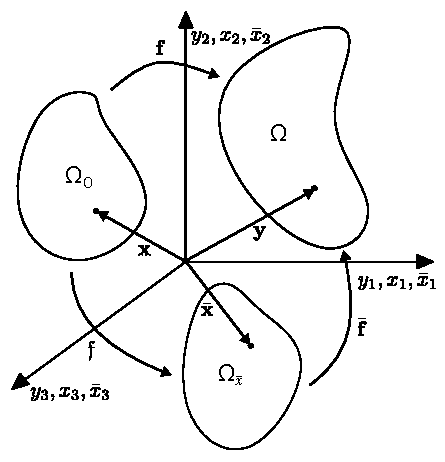
\includegraphics[scale=1.0]{Imagens/Cap2/dominioALE.pdf}	
	\end{center}
	\legend{Fonte: Elaborada pela autora}
	\label{fig:dominioAle}
\end{figure}

Da mesma forma, o domínio de referência pode ser mapeado a partir do domínio inicial por:

\begin{align}
	\posALE = \fmapRI(\posMat,t).
\end{align}

A velocidade dos pontos da malha é calculada por:

\begin{align}
	\velocityALE = \left. \frac{\partial \fmapAR(\posALE,t)}{\partial t} \right|_{\posALE},
\end{align}

\noindent e a velocidade dos pontos materiais no instante $t$ é obtida pela derivada do vetor posição $\pos$, mantendo $\posMat$ fixo:

\begin{align}
	\velocity = \left. \frac{\partial \fmapAI(\posMat,t)}{\partial t} \right|_{\posMat} = \left. \frac{\partial \pos(\posMat,t)}{\partial t} \right|_{\posMat}.
\end{align}

As matrizes jacobianas dos mapeamentos considerando a dependência do espaço e do tempo são dadas por:

\begin{equation} 
	\FmapAI = \frac{\partial \left(\fmapAI(\posMat,t),t\right)}{\partial (\posMat,t)}=
	\begin{bmatrix}
		\frac{\partial {\pos}}{\partial {\posMat}} & \velocity \\
		\vzero^T & 1 \\
	\end{bmatrix}
	\text{,}
\end{equation}

\begin{equation} 
	\FmapAR = \frac{\partial \left(\fmapAR(\posALE,t),t\right)}{\partial (\posALE,t)}=
	\begin{bmatrix}
		\frac{\partial {\pos}}{\partial {\posALE}} & \velocityALE \\
		\vzero^T & 1 \\
	\end{bmatrix}
	\text{,}
\end{equation}

\noindent e

\begin{equation}
	\FmapRI = \frac{\partial \left({\fmapRI}(\posMat,t),t\right)}{\partial (\posMat,t)}=
	\begin{bmatrix}
		\frac{\partial {\posALE}}{\partial {\posMat}} & \mathbf{w} \\
		\vzero^T & 1 \\
	\end{bmatrix}
	\text{,}
\end{equation}

\noindent sendo $\mathbf{w} = \left. \frac{\partial \posALE}{\partial t} \right|_{\posMat}$.

Considerando que $\fmapAI\left(\posMat,t\right) = \fmapAR \circ \fmapRI$, pode-se escrever:

\begin{align}
	\frac{\partial(\fmapAI(\posMat,t),t)}{\partial(\posMat,t)} = \frac{\partial(\fmapAR(\posALE,t),t)}{\partial(\posALE,t)} \cdot \frac{\partial(\fmapRI(\posMat,t),t)}{\partial(\posMat,t)},
\end{align}

\noindent que pode ser rescrita como:

\begin{align}
	\begin{bmatrix}
		\frac{\partial {\pos}}{\partial {\posMat}} & \velocity \\
		\vzero^T & 1 \\
	\end{bmatrix}
	=
	\begin{bmatrix}
		\frac{\partial {\pos}}{\partial {\posALE}} & \velocityALE \\
		\vzero^T & 1 \\
	\end{bmatrix}
	\cdot
	\begin{bmatrix}
		\frac{\partial {\posALE}}{\partial {\posMat}} & \mathbf{w} \\
		\vzero^T & 1 \\
	\end{bmatrix} .
\end{align}

Dessa forma, pode-se estabelecer uma relação entre a velocidade da malha e a velocidade do ponto material:

\begin{align}
	\velocity = \velocityALE + \frac{\partial{\pos}}{\partial{\posALE}}\cdot \mathbf{w}. \label{eq:vel_rel_mat_ALE}
\end{align}

Supondo agora uma grandeza física escalar, denominada $g(\pos,t)$ na configuração espacial, de $g^{*}(\posALE,t)$ na configuração de referência e $g^{**}(\posMat,t)$ na configuração material, pode-se escrever então:

\begin{align}
	g^{**}(\posMat,t) = g(\fmapAI(\posMat,t),t), 
\end{align}

\noindent ou:

\begin{align}
	g^{**} = g  \circ \fmapAI,
\end{align}

\noindent o que permite escrever o seguinte gradiente:

\begin{align}
	\frac{\partial g^{**}(\posMat,t)}{\partial (\posMat,t)} = \frac{\partial g(\pos,t)}{\partial (\pos,t)} \cdot \frac{\partial \fmapAI(\posMat,t)}{\partial (\posMat,t)},
\end{align}

\noindent que, em forma matricial, é apresentado como:

\begin{align}
	\begin{bmatrix}
		\frac{\partial {g^{**}}}{\partial {\posMat}} & \frac{\partial {g^{**}}}{\partial t} \\
	\end{bmatrix}
	=
	\begin{bmatrix}
		\frac{\partial {g}}{\partial \pos} & \frac{\partial {g}}{\partial t} 
	\end{bmatrix}
	\cdot
	\begin{bmatrix}
		\frac{\partial {\pos}}{\partial {\posMat}} & \velocity \\
		\vzero^T & 1 \\
	\end{bmatrix} .
\end{align}

Essa expressão nos permite escrever a derivada temporal da variável na configuração material:

\begin{align}
	\frac{\partial g^{**}}{\partial t} = \frac{\partial g}{\partial t} + \frac{\partial g}{\partial \pos} \cdot \velocity, 
\end{align}

\noindent que corresponde à derivada material de g. Para facilitar a visualização, podem-se remover os sobrescritos $**$, e então:

\begin{align}
	\frac{Dg}{Dt} = \left . \frac{\partial g}{\partial t} \right|_{\posMat} = \left . \frac{\partial g}{\partial t} \right|_{\pos} + \velocity \cdot \gradient g. \label{eq:der_mat}
\end{align}

Usando essa mesma metodologia, pode-se escrever a transformação de $g^{*}(\posALE,t)$ para a referência material da seguinte forma:

\begin{align}
	g^{**} = g^{*}  \circ \fmapRI,
\end{align}

\noindent que resulta no seguinte gradiente

\begin{align}
	\begin{bmatrix}
		\frac{\partial {g^{**}}}{\partial {\posMat}} & \frac{\partial {g^{**}}}{\partial t} \\
	\end{bmatrix}
	=
	\begin{bmatrix}
		\frac{\partial {g^*}}{\partial \posALE} & \frac{\partial {g*}}{\partial t} 
	\end{bmatrix}
	\cdot
	\begin{bmatrix}
		\frac{\partial {\posALE}}{\partial {\posMat}} & \mathbf{w} \\
		\vzero^T & 1 \\
	\end{bmatrix},
\end{align}

\noindent com a segunda coluna resultando em:

\begin{align}
	\frac{\partial g^{**}}{\partial t} = \frac{\partial g^*}{\partial t} + \frac{\partial g^*}{\partial \posALE} \cdot \mathbf{w}. \label{eq:ref_mat}
\end{align}

Utilizando-se a expressão apresentada na Equação \eqref{eq:vel_rel_mat_ALE} e substituindo-a na Equação \eqref{eq:ref_mat}, resulta em:

\begin{align}
	\frac{\partial g^{**}}{\partial t} = \frac{\partial g^*}{\partial t} + \frac{\partial g^*}{\partial \pos} \cdot \left(\velocity - \velocityALE \right). 
\end{align}

Removendo-se os sobrescritos (** e *), chega-se a equação fundamental para os desenvolvimentos utilizando a metodologia ALE:

\begin{align}
	\frac{Dg}{Dt} = \left . \frac{\partial g}{\partial t} \right|_{\posMat} = \left . \frac{\partial g}{\partial t} \right|_{\posALE} + \left(\velocity - \velocityALE \right) \cdot \gradient g. \label{eq:der_mat_ALE}
\end{align}

A partir da definição de derivada material da Equação \eqref{eq:der_mat} e comparando com a Equação \eqref{eq:Navier-Stokes}, pode-se rescrever a equação da quantidade de movimento da seguinte forma:

\begin{align}
	\density\left(\frac{D\velocity}{Dt} - \sbodyforce \right) - \divergence \cdot \stressTensor &= \vzero. \label{eq:Navier-Stokes_der_mat_Euleriana}
\end{align}

Para expressar a equação da quantidade de movimento em uma descrição Euleriana-Lagrangeana, basta substituir na Equação \eqref{eq:Navier-Stokes_der_mat_Euleriana} a definição de derivada material apresentada na Equação \eqref{eq:der_mat_ALE}, resultando:

\begin{align}
	\density\left(\left. \frac{\partial\velocity}{\partial t} \right|_{\posALE} + \left(\velocity - \velocityALE \right) \cdot \gradient  \velocity  - \sbodyforce \right) - \divergence \cdot \stressTensor = \vzero. \label{eq:Navier-Stokes_ALE} 
\end{align}

A equação da continuidade é independente da movimentação da malha. Dessa forma, a Equação \eqref{eq:conser_massa_incom} permanece válida para análises usando uma descrição ALE.

\subsection{Forma forte do modelo para escoamentos incompressíveis com contornos móveis}

Nesta seção é apresentado o problema para escoamentos incompressíveis com contornos móveis, assumindo-se que a velocidade da malha (do domínio de referência) é inteiramente conhecida. Posteriormente será desenvolvido o modelo matemático adotado para a movimentação da malha.

Seja $\domain \in \nrealspace$, com $\nsd = 1,2,3$ definindo a dimensão do domínio espacial do escoamento com contorno $\boundary = \boundaryD \cup \boundaryN$, no instante $t \in (0,\totalTime)$ (ver \autoref{fig:dominioFluido}).

Para escoamentos incompressíveis isotérmicos o fluido possui movimento descrito pela equação da quantidade de movimento, (Equação \eqref{eq:Navier-Stokes_der_mat_Euleriana}) e da continuidade (Equação \eqref{eq:conser_massa_incom}). Para completar a formulação da mecânica dos fluidos, condições de contorno devem ser especificadas. Em geral, em uma dada parte do contorno espacial, condições de contorno essenciais (Dirichlet) ou naturais (Neumann) são aplicadas. Dessa forma, o escoamento é governado pelo seguinte conjunto de equações:

\begin{equation}
	\left\{
	\begin{array}{l}
		\density\left( \left. \frac{\partial\velocity}{\partial t} \right|_{\posALE}  + \left(\velocity - \velocityALE \right)\cdot\gradient\velocity - \sbodyforce \right) - \divergence \cdot \stressTensor = \vzero  \ \textrm{em} \ \domain\\
		\divergence \cdot \velocity = 0  \ \textrm{em} \ \domain\\
		\velocity = \velocityD \ \textrm{em} \ \boundaryD \\
		\stressTensor \cdot \snormal = \surfaceLoad \ \textrm{em} \ \boundaryN,
	\end{array} \label{eq:conj_eq_DFC_ALE}
	\right.
\end{equation}

\noindent onde $\stressTensor$ é obtido por meio da Equação \eqref{eq:tensor_tensoes_fluido}, sendo $\boundaryD$ a porção do contorno sobre a qual são impostas as condições de contorno de Dirichlet, representadas pela distribuição de velocidade prescrita $\velocityD$, e $\boundaryN$ a porção com condições de Neumann, descritas pelas forças de superfície $\surfaceLoad$. A variável $\snormal$ representa o vetor unitário normal ao contorno $\boundaryN$.

\begin{figure}[H]
	\caption{Domínio para o problema da DFC}
	\begin{center}
		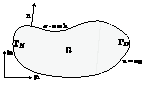
\includegraphics[scale=3.0,trim=0cm 0.0cm 0cm 0.0cm, clip=true]{Imagens/Cap2/dominioFluido.pdf}	
	\end{center}
	\legend{Fonte: Elaborada pela autora}
	\label{fig:dominioFluido}
\end{figure}


\section{Forma fraca e discretização espacial das equações governantes} \label{capitulo:Cap2:FormaFraca}

Tomando-se a forma forte das equações governantes da DFC em descrição ALE, aplica-se o método dos resíduos ponderados para se chegar à forma fraca e proceder com a discretização espacial. Os espaços de dimensão finita das funções tentativa que descrevem a velocidade e a pressão são chamados de $\usolution$ e $\psolution$ respectivamente, e definidos como:

\begin{align}
\usolution = \left\{\velocity \left . \right| \velocity \left(\cdot,t\right) \in \left(H^{1}\left(\domain\right)\right)^{\nsd}, \velocity = \velocity_D \ \textrm {em} \ \boundaryD \right\}
\end{align}

\noindent e

\begin{align}
\psolution = \left\{\press \left . \right| \press \left(\cdot\right) \in L^{2}\left(\domain\right), \int_{\domain}\press \textrm { } \deriv \domain = 0 \textrm { se } \boundary = \boundaryN \right\},
\end{align}

\noindent sendo $\left(H^{1}\left(\domain\right)\right)^{\nsd}$ o espaço de funções vetoriais com derivadas de quadrado integrável sobre $\domain$ e $L^{2}\left(\domain\right)$ o espaço de funções escalares de quadrado integrável sobre $\domain$.

Os espaços das funções teste (ou funções ponderadoras) das equações da quantidade de movimento e da continuidade são definidos, respectivamente, por:

\begin{align}
\uweighting = \left\{\utest \left . \right| \utest \left(\cdot\right) \in \left(H^{1}\left(\domain\right)\right)^{\nsd}, \utest = \vzero \textrm { em} \ \boundaryD \right\},
\end{align}

\begin{align}
\pweighting = \psolution.
\end{align}

Aplicando-se o método dos resíduos ponderados às equações Equação \eqref{eq:Navier-Stokes_ALE} e Equação \eqref{eq:conser_massa_incom}, integrando-se por partes o termo referente ao tensor de tensões de Cauchy, empregando-se o teorema da divergência e levando-se em consideração a condição de homogeneidade da função $\utest$ sobre o contorno $\boundaryD$, obtém-se a forma fraca do problema, dada por:

\begin{align}
\int_{\domain} \utest \cdot \density  \left(\left . \frac{\partial\velocity}{\partial t} \right|_{\posALE} + \left(\velocity - \velocityALE \right)\cdot\gradient \velocity - \sbodyforce \right) \deriv \domain + \int_{\domain} \straintensor(\utest) : \stressTensor  \deriv \domain - \int_{\boundaryN} \utest \cdot \surfaceLoad \deriv\boundaryN  \  &= 0,  \label{eq:QM_forma_fraca_0_cap2} 
\end{align}

\noindent e

\begin{align}
\int_{\domain} \ptest \left(\divergence \cdot \velocity\right) \deriv \domain &= 0. \label{eq:C_forma_fraca_0_cap2} 
\end{align}

A solução do problema consiste, então, em encontrar $\velocity \in \usolution$ e $\press \in \psolution$, de modo que para todo $\utest \in \uweighting$ e para todo $\ptest \in \pweighting$, Equação \eqref{eq:QM_forma_fraca_0_cap2} e Equação \eqref{eq:C_forma_fraca_0_cap2} sejam verdadeiras.

\subsection{Método dos elementos finitos } \label{capitulo:Cap2:FormaFraca:ElementosFinitos}

Antes de prosseguir com a discretização espacial da forma fraca do conjunto de equações da Mecânica dos Fluidos, é fundamental compreender os princípios básicos do Método dos Elementos Finitos.  A discretização espacial tanto pelo método dos elementos finitos, como pela técnica de análise isogeométrica (\autoref{capitulo:Cap3}), baseia-se em tomar um problema contínuo com domínio $\domain$ e representá-lo por um domínio $\domainh$ que é dividido em subdomínios $\domainE$, também chamados de elementos ou células, de forma que:

\begin{align}
	\domain \approx \domainh = {\bigcup_{e = 1}^{\nel}} \domainE,
\end{align}

\noindent onde $\nel$ representa o número total de elementos.

Da mesma forma, o contorno de $\domain$ é aproximado da seguinte forma:

\begin{align}
	\boundary \approx \boundaryh = {\bigcup_{b = 1}^{\neb}} \boundary^{b},
\end{align}

\noindent onde $\neb$ representa o número de faces ou lados de elementos que formam o contorno.

No Método dos Elementos Finitos, cada elemento é definido com auxílio de um conjunto de pontos chamados nós. As variáveis de interesse do problema, que incluem a geometria na abordagem isoparamétrica, são aproximadas pela combinação linear de um número finito de funções associadas aos nós, chamadas funções de forma, multiplicadas por variáveis denominadas parâmetros nodais. As funções de forma utilizadas no Método dos Elementos Finitos tradicionalmente satisfazem a propriedade de partição da unidade, ou seja, a soma das funções de forma associadas a todos os nós de um elemento resulta em 1 para qualquer ponto dentro do seu domínio. A técnica de elementos finitos pode ser encontrada nos diversos livros disponíveis sobre o assunto, tais como \citeonline{Reddy:2006} e \citeonline{ZienkiewiczTN:2005a}.

Nesse trabalho, para a mecânica dos fluidos, são utilizadas funções de forma quadráticas do tipo polinômios de Lagrange, sendo empregados elementos isoparamétricos triangulares para o caso 2D e tetraédricos para o caso 3D. Esses elementos são apresentados na Figura \ref{fig:elementoFinito2d} e Figura \ref{fig:elementoFinito3d}, onde são ilustrados também as coordenadas paramétricas adimensionais adotados para definir as funções de forma. 

\begin{figure}[!htbp]
	\caption{Elementos Finitos: representação espacial e paramétrica}
	\centering	
	\subfloat[Elemento Finito 2d\label{fig:elementoFinito2d}]{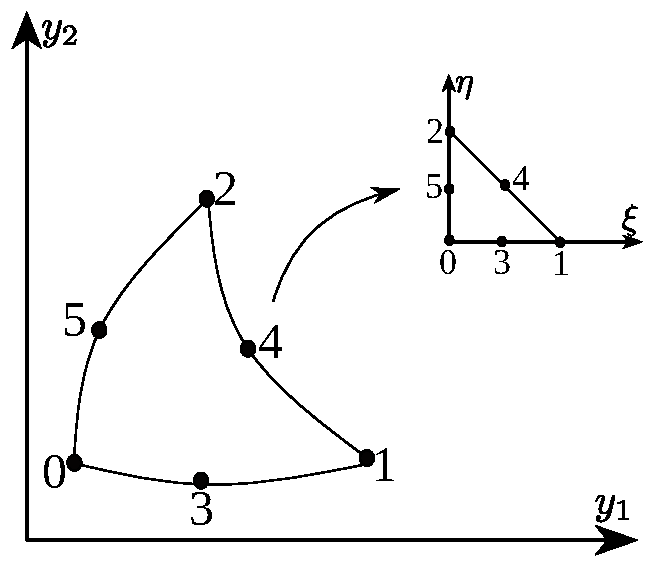
\includegraphics[scale=0.5,trim=0cm 0cm 0cm 0cm, clip=true]{Imagens/Cap2/elementoFinito2d.pdf}}\\
	\subfloat[Elemento Finito 3d\label{fig:elementoFinito3d}]{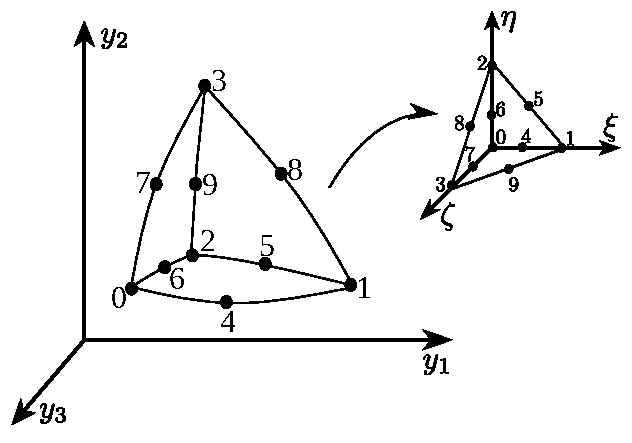
\includegraphics[trim=0 0 0 0,clip,scale=0.65]{Imagens/Cap2/elementoFinito3d.pdf}}
	\legend{Fonte: Elaborada pela autora}
\end{figure}

Adotar a abordagem isoparamétrica implica que a geometria do problema é descrita também pela combinação entre funções de forma e as coordenadas nodais da malha, ou seja:

\begin{align}
	\pos^{h}(\coordAdimen) = \sum_{a = 1}^{\nnos} \pos_{a}\shapef_{a}(\adimensionalcoordinates),  \label{eq:interp_geo}
\end{align}

\noindent sendo que para uma geometria tridimensional o vetor $\pos$ possui coordenadas $y_1,y_2$ e $y_3$, as quais representam as posições atuais dos pontos que compõem o domínio. O subíndice "$a$" $ \ $ representa o índice dos nós da malha, $\nnos$ o número total de nós e $\shapef$ as funções de forma da discretização.


\subsection{Discretização espacial} \label{capitulo:Cap2:DiscEspacial}

As funções tentativa para velocidade e pressão, bem as funções teste, assim com as coordenadas (Equação \eqref{eq:interp_geo}) são dadas pela combinação linear das funções de forma definidas sobre cada subdomínio:

\begin{align}
	\velocityh(\pos,t) = \sum_{a = 1}^{\nnos} \velocity_{a}(t)\shapef_{a}(\adimensionalcoordinates), \label{eq:interp_vel}
\end{align}

\begin{align}
	\pressh(\pos,t)  = \sum_{a = 1}^{\nnos} \press_{a}(t)\shapef_{a}(\adimensionalcoordinates),\label{eq:interp_press} 
\end{align}

\begin{align}
	\utesth(\pos)  = \sum_{a = 1}^{\nnos} \utest_{a}\shapef_{a}(\adimensionalcoordinates) \label{eq:interp_utest}
\end{align}

\noindent e
\begin{align}
	\ptesth(\pos)  = \sum_{a = 1}^{\nnos} \ptest_{a}\shapef_{a}(\adimensionalcoordinates). \label{eq:inter_ptest} 
\end{align}

O problema passa a ser enunciado como: Encontrar $\velocityh \in \usolutionh$ e $\pressh \in \psolutionh$, de tal modo que $\forall$ $\utesth \in \uweightingh$ e $\ptesth \in \pweightingh$ a seguinte expressão seja verdadeira:

\begin{align}
	\begin{split}
		&\int_{\domain} \utesth \cdot \density \left(\left. \frac{\partial\velocityh}{\partial t} \right|_{\posALE} + \left(\velocityh - \velocityALEh \right)\cdot\gradient \velocityh - \sbodyforceh \right) \deriv \domain + \int_{\domain} \straintensor(\utesth) : \stressTensor\left(\velocityh,\pressh \right)  \deriv \domain\\ & - \int_{\boundaryN} \utesth \cdot \surfaceLoadh \deriv \boundaryN \ + \int_{\domain} \ptesth \left(\divergence \cdot \velocityh\right) d \domain = 0.  \label{eq:QM_C_forma_fraca_1} 
	\end{split}
\end{align}

\noindent sendo as variáveis $\utest_{a}$ e $\ptest_{a}$ arbitrárias nas aproximações, enquanto $\velocity_{a}$ e $\press_{a}$ são as incógnitas a serem determinadas.

No entanto, as formulações obtidas pelo método de Bubnov-Galerkin são conhecidas por apresentarem oscilações espúrias em escoamentos dominados pela convecção. Uma das formas de se lidar com esse problema é a utilização de métodos estabilizados, como o \textit{Streamline-Upwind/Petrov-Galerkin} (SUPG) \cite{BrooksH:1982, HughesT:1984}. Essa metodologia consiste em adicionar à equação da quantidade de movimento, o seu resíduo ponderado por $\SUPG \left(\left(\velocityh - \velocityALEh \right) \cdot \gradient \utesth\right)$, onde $\SUPG$ é um parâmetro calculado para garantir bom condicionamento ao sistema. Do ponto de vista numérico, isso adiciona termos estabilizantes na direção das linhas de corrente, mantendo a formulação consistente por ser baseado na adição do resíduo ponderado.

Para os problemas de escoamentos incompressíveis aqui analisados, deve-se levar em conta que os campos de velocidade e pressão não podem ser aproximados arbitrariamente, podendo levar à ocorrência de oscilações espúrias no campo de pressão e instabilidade na solução. Para evitar isso, podem ser escolhidos elementos Taylor-Hood que obedeçam à condição de \textit{Ladyzhenskaya-Babuška-Brezzi} (LBB) \cite{BrezziF:1991,StrangF:2008,ZienkiewiczTN:2005b}, ou pode-se recorrer a um método estabilizado. 

Para conferir maior flexibilidade ao programa, opta-se pela formulação estabilizada com a técnica \textit{Pressure Stabilization Petrov Galerkin} (PSPG)  \cite{HughesFB:1986,TezduyarMRS:1992a}. Essa técnica consiste em adicionar à equação da continuidade, o resíduo da equação da quantidade de movimento ponderado pela função $\PSPG \left(\frac{\gradient \ptesth}{\density}\right)$, onde $\PSPG$ é um parâmetro calculado para garantir bom condicionamento ao sistema. Essa técnica introduz termo dependente da pressão na equação da continuidade, que é responsável pela estabilização, contornando a condição LBB.

Por fim, para prover maior estabilização em problemas com formação de vórtices, adiciona-se à equação da quantidade de movimento o resíduo da equação da continuidade ponderado por $ \LSIC \density \left(\divergence \cdot \utesth\right)$, sendo $\LSIC$ um parâmetro de estabilização. Essa estabilização, denominada \textit{Least Squares on Incompressibility Constraint LSIC} (LSIC), dá origem a um termo do tipo mínimos quadrados que introduz, de forma consistente, maior estabilidade à formulação \cite{BazilevsTT:2013a,TezduyarO:2000}.

Nota-se que a consistência da formulação com SUPG, PSPG e LSIC é garantida, uma vez que são adicionados às equações seus resíduos ponderados. 

Assim, o problema da dinâmica dos fluidos na formulação estabilizada, passa a ser a determinação de $\velocityh \in \usolutionh$ e $\pressh \in \psolutionh$, de tal modo que $\forall$ $\utesth \in \uweightingh$ e $\ptesth \in \pweightingh$ as seguintes expressões sejam verdadeiras:

\begin{align}
	\begin{split}
		&\int_{\domain} \utesth \cdot \density\left(\left. \frac{\partial\velocityh}{\partial t}\right|_{\posALE}+ \left(\velocityh - \velocityALEh \right) \cdot \gradient \velocityh - \sbodyforceh\right) \deriv \domain +\int_{\domain} \straintensor \left(\utesth\right) : \stressTensor \left(\velocityh,\pressh\right)\ \deriv \domain\\ &
		- \int_{\boundaryN}\utesth \cdot \surfaceLoadh \ \deriv \boundaryN 
		+ \sum_{e=1}^{\nel} \int_{\domainE} \SUPG \left(\left(\velocityh - \velocityALEh \right) \cdot \gradient \utesth\right) \cdot \resMom\left(\velocityh,\pressh \right)\  \deriv \domain\\
		&+ \sum_{e=1}^{\nel} \int_{\domainE} \density \LSIC \divergence \cdot \utesth \resPre\left(\velocityh\right)\  \deriv \domain = 0,
		\label{eq:QM_forma_fraca}
	\end{split}
\end{align}

\noindent e

\begin{align}
	\begin{split}
		&\int_{\domain}\ptesth \divergence \cdot \velocityh \ \deriv \domain
		+ \sum_{e=1}^{\nel} \int_{\domainE} \PSPG \left(\frac{\gradient \ptesth}{\density}\right) \cdot \resMom\left(\velocityh,\pressh\right) \  \deriv \domain = 0,
		\label{eq:C_forma_fraca}
	\end{split}
\end{align}

\noindent onde $\resMom$ e $\resPre$ são os resíduos da equação da quantidade de movimento e da equação da continuidade, respectivamente, dados por:

\begin{align}
	\resMom\left(\velocityh,\pressh\right)&=\density\left(\left. \frac{\partial\velocityh}{\partial t}\right|_{\posALE}+\left(\velocityh - \velocityALEh \right)\cdot \gradient \velocityh - \sbodyforceh\right) - \divergence \cdot \stressTensor\left(\velocityh,\pressh\right),
\end{align}

\noindent

\begin{align}
	\resPre\left(\velocityh\right)&=\divergence \cdot \velocityh.
\end{align}

Visto que existem funções teste separadas para a velocidade e pressão, pode-se definir dois vetores residuais correspondentes a equação da quantidade de movimento ($\NNSM$) e a equação da continuidade ($\NNSC$). Considerando a arbitrariedade de $\utest_{a}$ e $\ptest_{a}$, têm-se:

\begin{align}
	\NNSM  = [\left(\NNSM\right)_{a,i}],
\end{align}

\begin{align}
	\NNSC =  [\left(\NNSC\right)_{a}],
\end{align}

\noindent com:

\begin{align}
	\begin{split}
		\left(\NNSM\right)_{a,i} =&\int_{\domain} \shapef_{a}\mathbf{e_i} \cdot \density\left(\left. \frac{\partial\velocityh}{\partial t}\right|_{\posALE}+\left(\velocityh - \velocityALEh \right)\cdot \gradient \velocityh - \sbodyforceh\right) \deriv \domain +\int_{\domain} \straintensor \left(\shapef_{a}\mathbf{e_i}\right) : \stressTensor \left(\velocityh,\pressh\right)\ \deriv \domain\\ &
		- \int_{\boundaryN}\shapef_{a}\mathbf{e_i} \cdot \surfaceLoadh \ \deriv \boundaryN 
		+ \sum_{e=1}^{\nel} \int_{\domainE} \SUPG \left(\left(\velocityh - \velocityALEh \right) \cdot \gradient \shapef_{a}\mathbf{e_i}\right) \cdot \resMom\left(\velocityh,\pressh \right)\  \deriv \domain\\
		&+ \sum_{e=1}^{\nel} \int_{\domainE} \density \LSIC \left(\divergence \cdot \shapef_{a}\mathbf{e_i}\right) \resPre\left(\velocityh\right)\  \deriv \domain  ,
	\end{split}
\end{align}

\noindent e:

\begin{align}
	\begin{split}
		\left(\NNSC\right)_{a} = &\int_{\domain} \shapef_{a} \divergence \cdot \velocityh \ \deriv \domain  
		+ \sum_{e=1}^{\nel} \int_{\domainE} \PSPG \left(\frac{\gradient \shapef_{a}}{\density}\right) \cdot \resMom\left(\velocityh,\pressh\right) \  \deriv \domain,
	\end{split}
\end{align}

\noindent com $i=1,2$ para problemas 2D e $i=1,3$ para problemas 3D.

Considerando $\Acceleration$, $\Velocity$ e $\Press$ os vetores nodais dos graus de liberdade respectivos a velocidade, aceleração e pressão, pode-se escrever a forma semidiscreta do problema da DFC como: Encontrar $\Acceleration$, $\Velocity$ e $\Press$ de maneira que

\begin{align}
	\NNSM(\Acceleration,\Velocity,\Press) = \vzero,\label{eq:resid_semi_discr_QM}
\end{align}

\noindent e

\begin{align}
	\NNSC(\Acceleration,\Velocity,\Press) = \vzero. \label{eq:resid_semi_discr_C}
\end{align}

\subsection{Parâmetros de estabilização}\label{capitulo:Cap2:FormaFraca:taus}

A definição adequada dos parâmetros de estabilização desempenha papel fundamental no desempenho do método e na sua estabilidade numérica.

Desde os primeiros desenvolvimentos relacionados aos métodos estabilizados houve um amadurecimento das expressões de definição dos parâmetros $\tau$, as quais passam a levar em consideração formulações mais robustas, sendo adaptadas tanto para elementos de ordem elevadas, quanto para malhas mais complexas, como as usadas em análise isogeométrica.

Considerando que neste trabalho dois tipos de aproximações espaciais são utilizadas, uma baseada no FEM e outra baseada em AIG, adotam-se os parâmetros propostos mais recentemente por \citeonline{OtoguroTT:2020}, \citeonline{TakizawaTO:2018} e \citeonline{TakizawaUT:2019}, que são adequados para ambas aproximações. 

Para essa opção é necessário definir-se o tensor métrico do elemento no espaço. Com essa finalidade, descreve-se inicialmente a matriz Jacobiana $\matrixQ$, como:

\begin{align}
	\matrixQ&=\left(\frac{\partial\pos}{\partial\coordAdimen}\right),
\end{align}

\noindent com $\coordAdimen$ representando as coordenadas do espaço paramétrico, com componentes $\xi, \eta$ e $\zeta$.

Para que a ordem polinomial seja levada em consideração, ou, outros fatores como a dimensão do elemento no espaço paramétrico, aplica-se à $\matrixQ$, uma matriz de transformação ($\matrixD$), conforme a seguinte expressão:

\begin{align}
	\matrixQhat&=\matrixQ\matrixD^{-1} \label{eq:q_chap}.
\end{align}

O comprimento direcional do elemento fica definido como:

\begin{align}
	\RQD &=2\left(\rRGN\rRGN : \matrixG \right)^{-\frac{1}{2}},
\end{align}

\noindent o fator 2 vem de um típico espaço paramétrico, que é um quadrado ou um cubo com lado de comprimento 2. $\rRGN$ é o vetor unitário na direção do gradiente da intensidade da velocidade e $\matrixG$ o tensor métrico do elemento, os quais são representados respectivamente como:

\begin{align}
	\rRGN&=\frac{\gradient \lVert\velocityh - \velocityALEh\rVert}{\lVert \gradient \lVert\velocityh - \velocityALEh\rVert\rVert} \label{eq:rRGN}
\end{align}

\noindent e

\begin{align}
	\matrixG &= \matrixQhat^{-T} \cdot \matrixQhat^{-1}. \label{eq:tensor_metrico}
\end{align}

Para elementos finitos com funções de forma polinomiais de Lagrange de ordens $p_\xi$, $p_\eta$ e $p_\zeta$ nas direções paramétricas $\xi$, $\eta$ e $\zeta$, respectivamente, com $\xi, \eta, \zeta \in [-1, 1]$, a matriz $\mathbf{D}$ é definida por:

\begin{align}
	\matrixD&=\begin{bmatrix}
		p_{\xi} & 0 & 0\\
		0 & p_{\eta} & 0 \\
		0 & 0 & p_{\zeta}
	\end{bmatrix}.
\end{align}

Em geral, se escolhe o espaço paramétrico baseado em razões como eficiência da integração numérica ou conveniência de implementação. A maioria das metodologias utilizadas para definir o comprimento do elemento não levam este fator em consideração. Para essa finalidade, em \citeonline{TakizawaUT:2019}, apresenta-se a matriz de transformação ($\matrixD$) como:

\begin{align}
	\matrixD = \frac{\partial{\hat{\coordAdimen}}}{\partial{\coordAdimen}},
\end{align}

\noindent com $\hat{\coordAdimen}$ chamado de espaço de paramétrico de preferência.

Para elementos simplex, buscando encontrar uma expressão que leve a um comprimento de elemento que não possua variação em função da ordenação dos nós, os autores introduziram um espaço paramétrico preferido que consiste em um elemento simplex regular com distância entre vértices de 2, e chegaram a seguinte expressão para $\matrixD$ quando $\nsd = 2$:

\begin{align}
	\matrixD&= \frac{\sqrt{2}}{2} \begin{bmatrix}
		\sqrt{3} + 1 & \sqrt{3} - 1 \\
		\sqrt{3} - 1 & \sqrt{3} + 1
	\end{bmatrix},
\end{align}

\noindent e para $\nsd = 3$:

\begin{align}
	\matrixD&= \frac{\sqrt{2}}{3} \begin{bmatrix}
		4 & 1 & 1 \\
		1 & 4 & 1 \\
		1 & 1 & 4
	\end{bmatrix}.
\end{align}

A definição da matriz $\matrixD$ para elementos isogeométricos será descrita na \autoref{capitulo:Cap3:RepreGeo:taus2}.

Além disso, nessa metodologia, o comprimento do elemento é limitado pelos mínimos e máximos valores representados abaixo:

\begin{align}
	h_{min} \equiv 2\min_{r}\left((\rRGN\rRGN:\matrixG)^{-\frac{1}{2}} \right), \\
	h_{max} \equiv 2\max_{r}\left((\rRGN\rRGN:\matrixG)^{-\frac{1}{2}} \right),
\end{align}

\noindent que podem ser reescritos como:

\begin{align}
	h_{min} = 2\left(\lambda_{max}\matrixG\right)^{-\frac{1}{2}}, \\
	h_{max} = 2\left(\lambda_{min}\matrixG\right)^{-\frac{1}{2}},
\end{align}

\noindent onde $\lambda_{max}$ e $\lambda_{min}$ representam os máximos e mínimos autovalores da matriz $\matrixG$. 

Por fim, os parâmetros de estabilização são escritos como:

\begin{align}
	\SUPG = \PSPG =\left(\frac{1}{\SUGNi^2} + \frac{1}{\SUGNii^2} + \frac{1}{\SUGNiii^2} \right)^{-\frac{1}{2}},
\end{align}

\begin{align}
	\LSIC = \SUPG \lVert\velocityh - \velocityALEh\rVert^2,
\end{align}

\noindent onde:

\begin{align}
	\SUGNi^{-2} = \left(\velocityh - \velocityALEh \right) \left(\velocityh - \velocityALEh \right) : \matrixG ,
\end{align}

\begin{align}
	\SUGNii&=\frac{\timeStep}{2},
\end{align}

\noindent e

\begin{align}
	\SUGNiii^{-1} = \kviscosity \left(\rRGN_{reg}\rRGN_{reg} : \matrixG + \left(1 - \rRGN_{reg}^2)4h_{min}^{-2} \right)\right) ,
\end{align}

\noindent sendo $\rRGN_{reg}$ definido como:

\begin{align}
	\rRGN_{reg} =\frac{\gradient \lVert\velocityh - \velocityALEh\rVert}{\lVert \gradient \lVert\velocityh - \velocityALEh\rVert\rVert + \varepsilon\left(\lVert \gradient \lVert\velocityh - \velocityALEh\rVert\rVert\right)_0},
\end{align}

\noindent com $\varepsilon$ uma constante pequena e $\left(\lVert \gradient \lVert\velocityh- \velocityALEh\rVert\rVert\right)_0$ um valor de referência. Os termos $\SUGNi$, $\SUGNii$ e $\SUGNiii$ são parâmetros correspondentes aos termos convectivos, inerciais e viscosos, respectivamente.

\section{Integração temporal e solução numérica}\label{capitulo:Cap2:IntegTemp}

Para a integração temporal das equações governantes, utiliza-se o método $\alpha$-generalizado. Esse método foi proposto inicialmente por \citeonline{ChungH:1993} no contexto da mecânica das estruturas, e foi estendido para o contexto da dinâmica dos fluidos computacional por \citeonline{JansenWH:2000}.

Considerando que o tempo da análise do problema é definido por um intervalo temporal de $[0,\totalTime]$, o qual é particionado em $npt$ subintervalos $\timeStep_{n} = t_{n+1} - t_{n}$, com $t_{n}$ e $t_{n+1}$ os instantes anterior e atual, respectivamente. A solução do problema consiste em: conhecidos os valores nodais de aceleração, velocidade e pressão ($\Acceleration$, $\Velocity$ e $\Press$) no instante $n$, encontrar a solução no instante $n+1$ de forma que:

\begin{align}
\NNSM(\Acceleration_{n+\alpham},\Velocity_{n+\alphaf},\Press_{n+1}) = \vzero, \label{eq:resid_QM_alpha}\\
\NNSC(\Acceleration_{n+\alpham},\Velocity_{n+\alphaf},\Press_{n+1}) = \vzero, \label{eq:resid_cont_alpha}
\end{align}

\noindent com:

\begin{gather}
\Acceleration_{n+\alpham} = \Acceleration_n + \alpham \left( \Acceleration_{n+1} - \Acceleration_n \right), \label{eq:inter_acel}\\
\Velocity_{n+\alphaf} = \Velocity_n + \alphaf \left( \Velocity_{n+1} - \Velocity_n \right), \label{eq:inter_vel}
\end{gather}

\noindent sendo $\Acceleration_{n+\alpham}$ e $\Velocity_{n+\alphaf}$ valores intermediários entre $t_{n}$ e $t_{n+1}$ do vetor aceleração e velocidade. A relação entre os valores nodais de aceleração e velocidade são calculados de acordo com fórmula de Newmark (ver, por exemplo, \cite{Hughes:1976}):

\begin{gather}
\Velocity_{n+1} = \Velocity_n + \timeStep\left(\left(1-\gamma\right)\Acceleration_n + \gamma\Acceleration_{n+1} \right), \label{eq:Newmark}
\end{gather}

\noindent onde $\gamma$ é um parâmetro do método.

Os parâmetros que definem o instante intermediário, alteram as características de estabilidade e precisão ao método. Segundo \citeonline{JansenWH:2000}, precisão de segunda ordem é garantida, para problemas lineares, se: 

\begin{gather}
\gamma = 1/2 + \alpham - \alphaf,\label{eq:gamma}
\end{gather}

\noindent enquanto que a estabilidade do problema é incondicional com:

\begin{gather}
\alpham \ge \alphaf \ge 1/2.
\end{gather}

Para proporcionar a precisão de segunda-ordem de convergência, estabilidade incondicional da solução, e permitir dissipação ótima de altas frequências, calcula-se o parâmetro $\gamma$ de acordo com Equação \eqref{eq:gamma} e $\alpham$, $\alphaf$, através de \cite{Hughes:2000}:

\begin{gather}
\alpham = \frac{1}{2}\left(\frac{3 - \specRadius}{1+\specRadius}\right)\label{eq:alpha_m}
\end{gather}

\noindent e

\begin{gather}
\alphaf = \frac{1}{1+\specRadius}\label{eq:alpha_f}.
\end{gather}

O parâmetro $\specRadius$ é o raio espectral da matriz de amplificação quando $\timeStep \rightarrow \infty$, devendo estar contido no intervalo de $[0,1]$. Para $\specRadius = 0$ a dissipação de altas frequências é máxima e para $\specRadius = 1$ não há introdução de difusão numérica ao método.

Para a solução do sistema de equações não lineares compostas pela Equação \eqref{eq:resid_QM_alpha} e Equação \eqref{eq:resid_cont_alpha} utiliza-se o método de Newton-Raphson. O método pode ser separado em duas etapas, uma etapa preditiva e outra iterativa corretiva \cite{BazilevsTT:2013a}.

Na etapa preditiva, conhecida a solução em um passo de tempo $n$, prediz-se a solução em $n+1$ com as seguintes equações:

\begin{align}
\Acceleration_{n+1}^{0} = \frac{\gamma-1}{\gamma}\Acceleration_{n} \label{eq:pred_acel},
\end{align}

\begin{align}
\Velocity_{n+1}^{0} = \Velocity_{n}, \label{eq:pred_vel}
\end{align}

\begin{align}
\Press_{n+1}^{0} = \Press_{n},\label{eq:pred_press}
\end{align}

\noindent onde o índice $0$ representa a iteração de número zero. 

Na etapa iterativa corretiva, itera-se sobre a Equação \eqref{eq:resid_QM_alpha} e Equação \eqref{eq:resid_cont_alpha} até que elas sejam satisfeitas, considerando uma tolerância prescrita, ou até que se alcance uma quantidade máxima de iterações pré-estabelecida. Essa etapa é composta por três fases. A fase 1 consiste em determinar os valores no instante intermediário para as variáveis nodais na iteração $i$:

\begin{align}
\Acceleration_{n+\alpham}^{i} = \Acceleration_n + \alpham \left( \Acceleration_{n+1}^{i} - \Acceleration_n \right), \label{eq:inter_acel_i}\\
\Velocity_{n+\alphaf}^{i} = \Velocity_n + \alphaf \left( \Velocity_{n+1}^{i} - \Velocity_n \right), \label{eq:inter_vel_i}\\
\Press_{n+1}^{i} = \Press_{n+1}^{i} \label{eq:inter_press_i}.
\end{align}

Na fase 2, com os valores intermediários das variáveis nodais resolve-se o sistema linear resultante da linearização da Equação \eqref{eq:resid_QM_alpha} e Equação \eqref{eq:resid_cont_alpha} com respeito às variáveis de interesse $\Press_{n+1}$ e $\Acceleration_{n+1}$:

\begin{align}
\left .\frac{\partial\NNSM}{\partial\Acceleration_{n+1}}\right|_{i} \Delta \Acceleration_{n+1}^{i} + \left .\frac{\partial\NNSM}{\partial\Press_{n+1}}\right|_{i} \Delta \Press_{n+1}^{i} = -\NNSM^{i}, \label{eq:eq_lin_QM} \\
\left .\frac{\partial\NNSC}{\partial\Acceleration_{n+1}}\right|_{i} \Delta \Acceleration_{n+1}^{i} + \left .\frac{\partial\NNSC}{\partial\Press_{n+1}}\right|_{i} \Delta \Press_{n+1}^{i} = -\NNSC^{i}.\label{eq:eq_lin_cont}
\end{align}

Por fim, na fase 3 atualiza-se a solução através das seguintes relações:

\begin{align}
\Acceleration_{n+1}^{i+1} = \Acceleration_{n+1}^{i} + \Delta\Acceleration_{n+1}^{i},\label{eq:atu_acel} \\ 
\Velocity_{n+1}^{i+1} = \Velocity_{n+1}^{i} + \gamma \timeStep \Delta\Velocity_{n+1}^{i},\label{eq:atu_vel}\\
\Press_{n+1}^{i+1} = \Press_{n+1}^{i} + \Delta\Press_{n+1}^{i}.\label{eq:atu_press}
\end{align}

Na utilização do método $\alpha$-generalizado as integrais da Equação \eqref{eq:resid_QM_alpha} e Equação \eqref{eq:resid_cont_alpha} são avaliadas no instante $t = t_{n+\alpha_{f}}$, de forma que:

\begin{align}
\int_{\domain} \left(.\right) \deriv \domain = \int_{\domainALEN} \left(.\right) \deriv \domain,
\end{align}

\noindent e, por consequência:

\begin{align}
\domainALEN = \left\{\posh \  |\  \posh(\posALEh,t_{(n+\alphaf)}) = \alphaf \posh(\posALEh,t_{n+1}) + (1-\alphaf) \posh(\posALEh,t_n)  \right\}.
\end{align}

Finalmente, é possível estabelecer o algoritmo para a solução dos problemas de escoamentos incompressíveis com a formulação estabilizada do MEF, o qual é apresentado abaixo (Algoritmo. \ref{alg:fluid}).

\begin{algorithm}
	\caption{Algoritmo para problemas de dinâmica dos fluidos computacional}
	\label{alg:fluid}
	\begin{algorithmic}[1]
		\For {o passo de tempo $0$ até $npt-1$} 
		\State $i=0$;
		\State Predição da solução: aplicação da Equação \eqref{eq:pred_acel}, Equação \eqref{eq:pred_vel} e Equação \eqref{eq:pred_press};
		\While{($\epsilon$ < tolerância)}
		\State $i=i+1$;
		\State Interpolação das variáveis do problema: aplicação da Equação \eqref{eq:inter_acel_i}, Equação \eqref{eq:inter_vel_i} e Equação \eqref{eq:inter_press_i};
		\State Cálculo do incremento nas variáveis do problema: $\Acceleration_{n+1}$ e $\Press_{n+1}$ de acordo com a Equação \eqref{eq:eq_lin_QM} e Equação \eqref{eq:eq_lin_cont};
		\State Atualização da solução: calculadas de acordo com a Equação \eqref{eq:atu_acel}, Equação \eqref{eq:atu_vel} e Equação \eqref{eq:atu_press}.
		\State Cálculo do erro:
		\begin{align}
		\epsilon =\left\| \NNSM^i \right\|_{L^2}
		\end{align}
		\EndWhile
		\State Atualização das variáveis do passo anterior;
		\EndFor
	\end{algorithmic}
\end{algorithm}

\section{Verificação e aplicações} \label{capitulo:Cap2:VerApl}

Para a verificação do código baseados no método dos elementos finitos são simulados 2 exemplos amplamente estudados na literatura: escoamento sobre um cilindro e escoamento sobre uma cavidade quadrada.

\subsection{Escoamento sobre um cilindro} \label{capitulo:Cap2:VerApl:Cilindo}

Este exemplo considera um escoamento viscoso incompressível sobre um cilindro rígido com diferentes números de Reynolds, $\Reynolds = 40$, $\Reynolds = 100$ e $\Reynolds = 1000$, calculados de acordo com:

\begin{align}
	\Reynolds = \frac{\density L \lVert\velocinfty\lVert}{\viscosity} = \frac{L \lVert \velocinfty \lVert}{\kviscosity}, \label{eq:Reynolds}
\end{align}

\noindent onde a dimensão característica do problema $L$ é adotada como sendo o diâmetro do cilindro, e $\kviscosity$ é a viscosidade cinemática do fluido. Tomam-se como parâmetros de análise os coeficientes aerodinâmicos medidos ao longo do tempo, e avalia-se se o modelo é capaz de reproduzir os fenômenos relacionados à formação e desprendimento de vórtices característicos desse problema. 

A geometria e as condições de contorno são apresentadas na Figura \ref{fig:cilindro_geometria}, tratando-se de um domínio retangular, parametrizado em função do diâmetro do cilindro, com um perfil constante de velocidade na entrada e condição de parede lisa nos limites superior e inferior. No contorno denominado como saída, aplica-se condição de Neumann nula. Na Figura \ref{fig:cilindro_malha} é apresentada a malha utilizada para esse problema, composta por 9122 elementos finitos triangulares de aproximação quadrática e 18508 nós. O problema foi simulado para um velocidade de entrada $u_{\infty} = 1,0$, densidade $\density = 1,0$, passo de tempo $\timeStep = 0,05$, e parâmetro do integrador temporal $\specRadius = 0,5$, variando-se a viscosidade em função do número de Reynolds. 

\begin{figure}[!htbp]
	\caption{Cilindro: Geometria, condições de contorno e malha de elementos finitos.}
	\begin{center}
	\subfloat[Geometria e condições de contorno\label{fig:cilindro_geometria}]{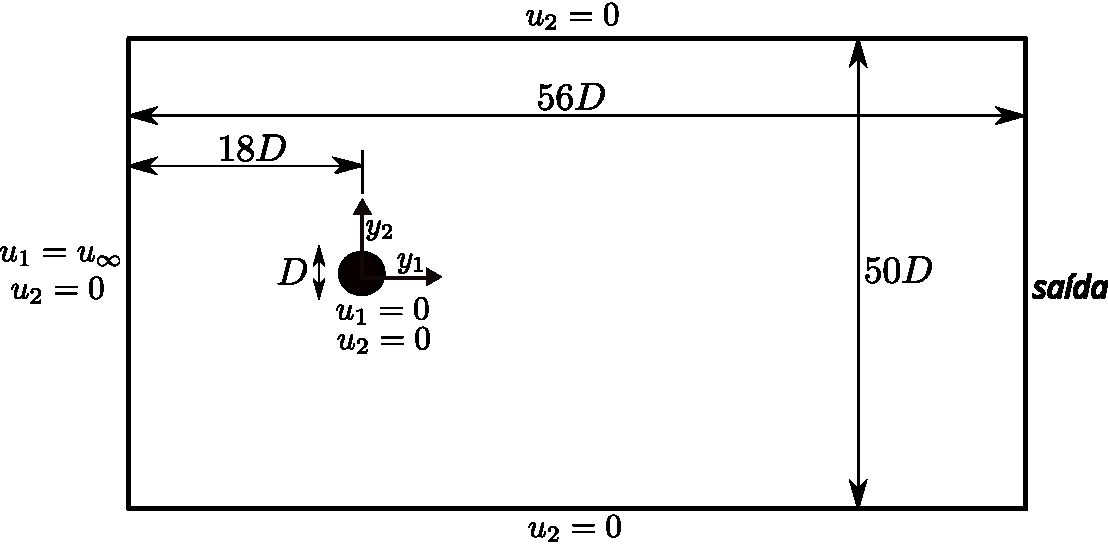
\includegraphics[scale=0.6,trim=0cm 0cm 0cm 0cm, clip=true]{Imagens/Cap2/cilindro_geometria.pdf}}\\
	\subfloat[Discretização espacial\label{fig:cilindro_malha}]{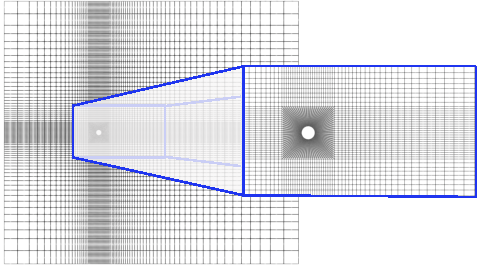
\includegraphics[trim=0cm 1cm 0cm 1cm,clip,scale=0.4]{Imagens/Cap2/cilindro_malha.pdf}}
	\end{center}
	\legend{Fonte: Elaborada pela autora}
\end{figure}

Para o cálculo dos coeficientes aerodinâmicos é necessário definir-se primeiramente as forças de arrasto ($F_D$) e de sustentação ($F_L$), as quais resultam das tensões de cisalhamento e da pressão, sendo calculadas pelas seguintes expressões:

\begin{align}
F_D = \int_{\boundary_{c}} \stressTensor_{1j}n_{j} \deriv\boundary_{c}, \label{eq:F_D}
\end{align}

\noindent e 

\begin{align}
F_L = \int_{\boundary_{c}} \stressTensor_{2j}n_{j} \deriv\boundary_{c},  \label{eq:F_L}
\end{align}

\noindent onde $\boundary_{c}$ representa o contorno do cilindro e $n_j$ é a componente $j$ do vetor unitário normal a $\boundary_{c}$, com $j=1,2$. Os coeficientes de arrasto e sustentação são definidos respectivamente por:

\begin{align}
	C_D = \frac{F_D}{0,5\density \lVert \velocinfty \lVert^{2} L},
\end{align}

\noindent e

\begin{align}
	C_L = \frac{F_L}{0,5\density \lVert \velocinfty \lVert^{2} L}.
\end{align}.

Para este problema, a frequência do desprendimento de vórtices que ocorre a partir de determinado número de Reynolds pode ser determinada a partir do número adimensional de Strouhal ($\Strouhal$), dado por:

\begin{align}
	\Strouhal = \frac{f_{v}L}{\lVert \velocinfty \lVert},
\end{align}.

\noindent com $f_{v}$ sendo a frequência de desprendimento dos vórtices.


Como pode-se observar na Figura \ref{fig:cilindro_coefAero}, para $\Reynolds = 40$ os coeficientes de arrasto atinge um valor constante, quando o escoamento fica estacionário, permanecendo assim até o final da análise, enquanto o coeficiente de sustentação permanece nulo. Isso é o que se espera, visto que para Reynolds entre 5 à 50, deve-se observar a formação de dois vórtices simétricos e estacionários na região à jusante do cilindro \cite{Lienhard:1966}. Com o aumento do número de Reynolds o par de vórtices é quebrado gerando a chamada esteira de von Kármán, com formação de vórtices de maneira alternada entre as regiões superior e inferior do cilindro, levando ao comportamento oscilatório observado nos gráficos para $\Reynolds = 100$ e $\Reynolds=1000$. Os valores do coeficiente de Strouhal, para $\Reynolds = 100$ e $\Reynolds=1000$, assim como os valores médios obtidos para o coeficiente de arrasto ($C_{Dmed}$) para $\Reynolds = 40$, $\Reynolds = 100$ e $\Reynolds = 1000$ são apresentados na \autoref{tab:cilindro_CD_ST}, onde são comparados com os valores de referência provenientes do trabalho de \citeonline{WANDERLEY2002445}.

\begin{figure}[!htbp]
	\caption{Cilindro: Coeficientes aerodinâmicos}
	\centering
	\subfloat[\label{fig:cilindro_Cd}Coeficiente de arrasto $ C_D$]{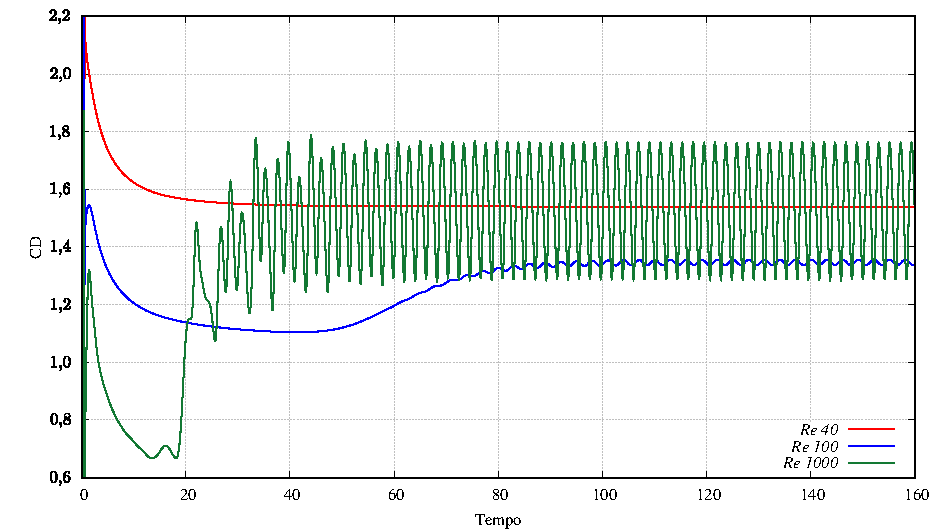
\includegraphics[scale=0.7,trim=0cm 0cm 0cm 0cm, clip=true]{Imagens/Cap2/cilindro_CD.pdf}}\\ 
	\subfloat[\label{fig:cilindro_Cl}Coeficiente de sustentação $C_L$]{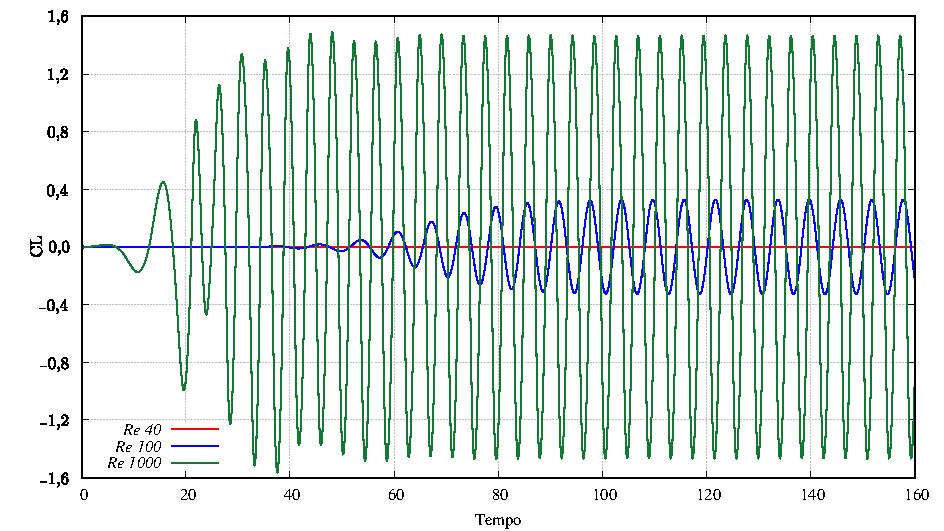
\includegraphics[scale=0.7,trim=0cm 0cm 0cm 0cm, clip=true]{Imagens/Cap2/cilindro_CL.pdf}}\\ 
	\label{fig:cilindro_coefAero}
	\legend{Fonte: Elaborada pela autora}
\end{figure}

\begin{table}[h!]
	\centering
	\caption{Comparação entre valores obtidos e valores de referência}
	\begin{tabular}{ccccc}
		\toprule
		\multirow{2}{*}{$Re$} & \multicolumn{2}{c}{$C_{Dmed}$} & \multicolumn{2}{c}{$St$} \\ \cline{2-5}
		& Presente estudo & Referência & Presente estudo & Referência \\ \midrule \midrule
		40   & 1,54  & 1,59 & - & - \\ \midrule
		100  & 1,35 &  1,33 & 0,166 & 0,163 \\ \midrule
		1000 & 1,52 &  1,51 & 0,238 & 0,235 \\ \bottomrule
	\end{tabular}
	\label{tab:cilindro_CD_ST}
	\fonte{Elaborada pela autora.}%
\end{table}


Nas Figura \ref{fig:cilindro_camposVel} e Figura \ref{fig:cilindro_camposPressao} são apresentados os campos de velocidade e pressão ao longo de um ciclo de desprendimento de vórtices $nT$ para $\Reynolds = 100$. Pode-se notar nessas imagens, a formação e o desprendimento de vórtices na esteira de Von Karmán.

\begin{figure}[!htbp]
	\caption{Cilindro: Campos de velocidade para $\Reynolds = 100$}
	\centering
	\subfloat[$nT$]{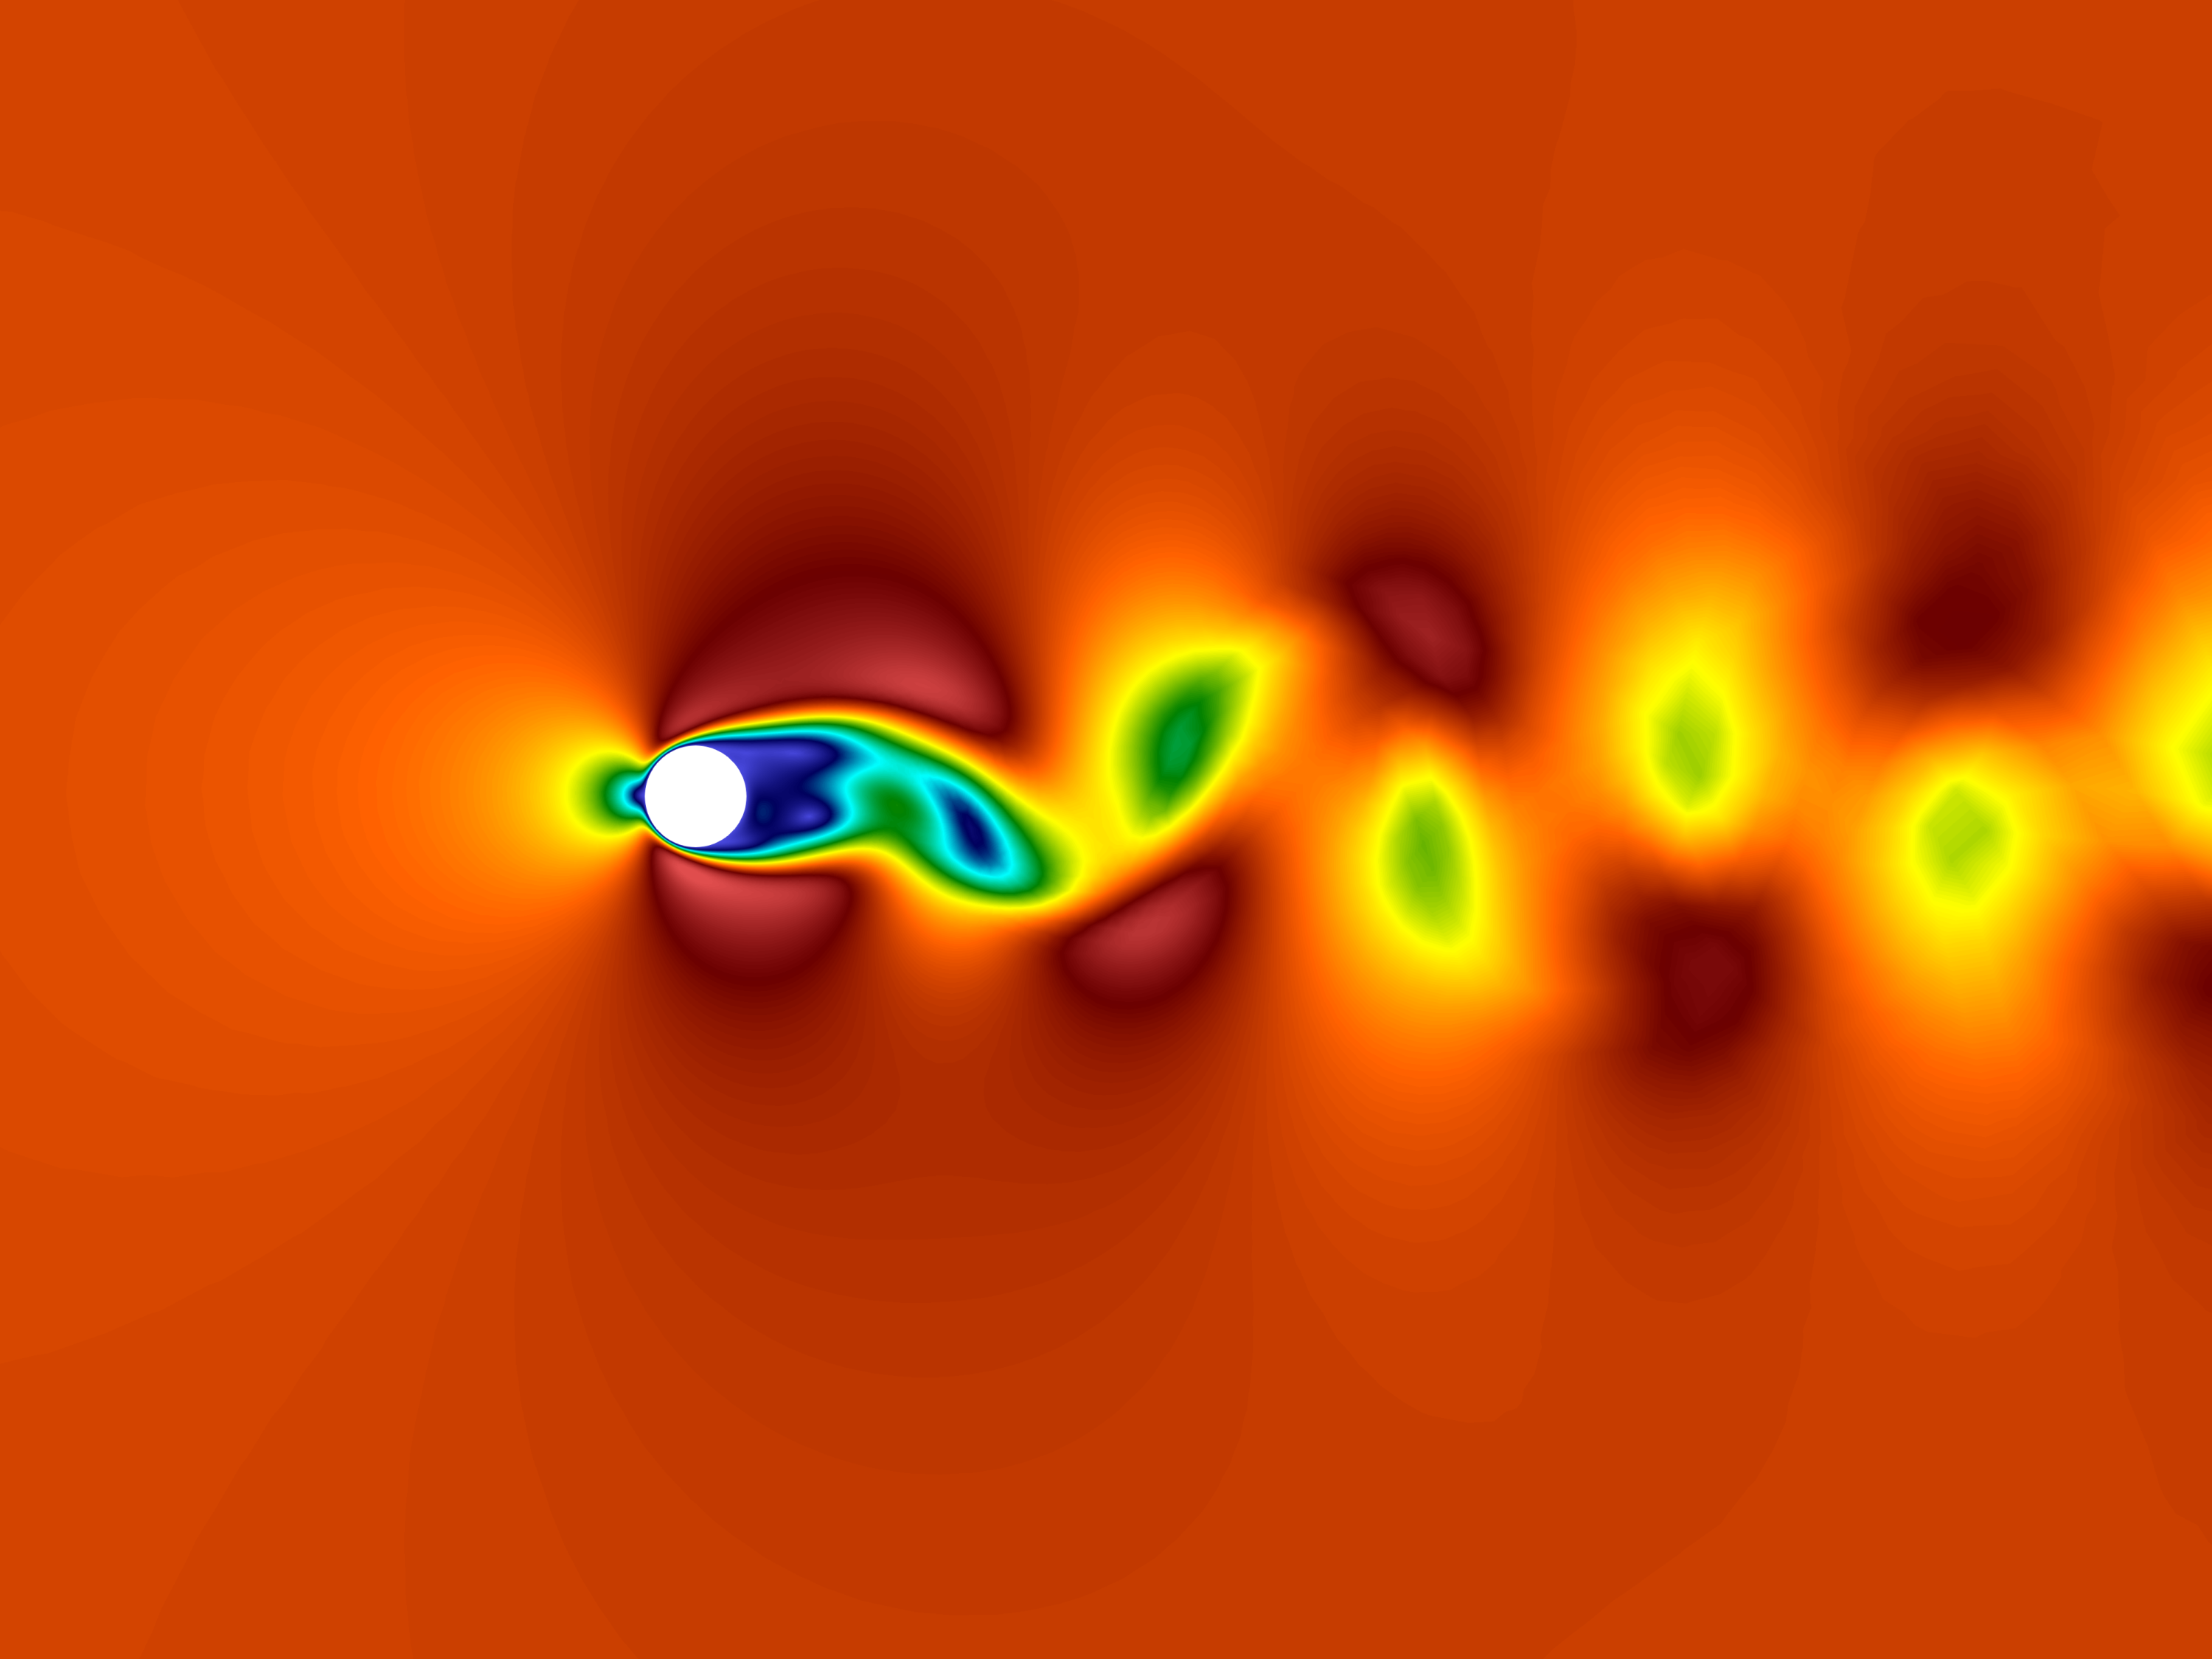
\includegraphics[scale=0.15,trim=5cm 5cm 5cm 6cm, clip=true]{Imagens/Cap2/cilindro_vel2020.pdf}} \
	\subfloat[$nT + nT/6$]{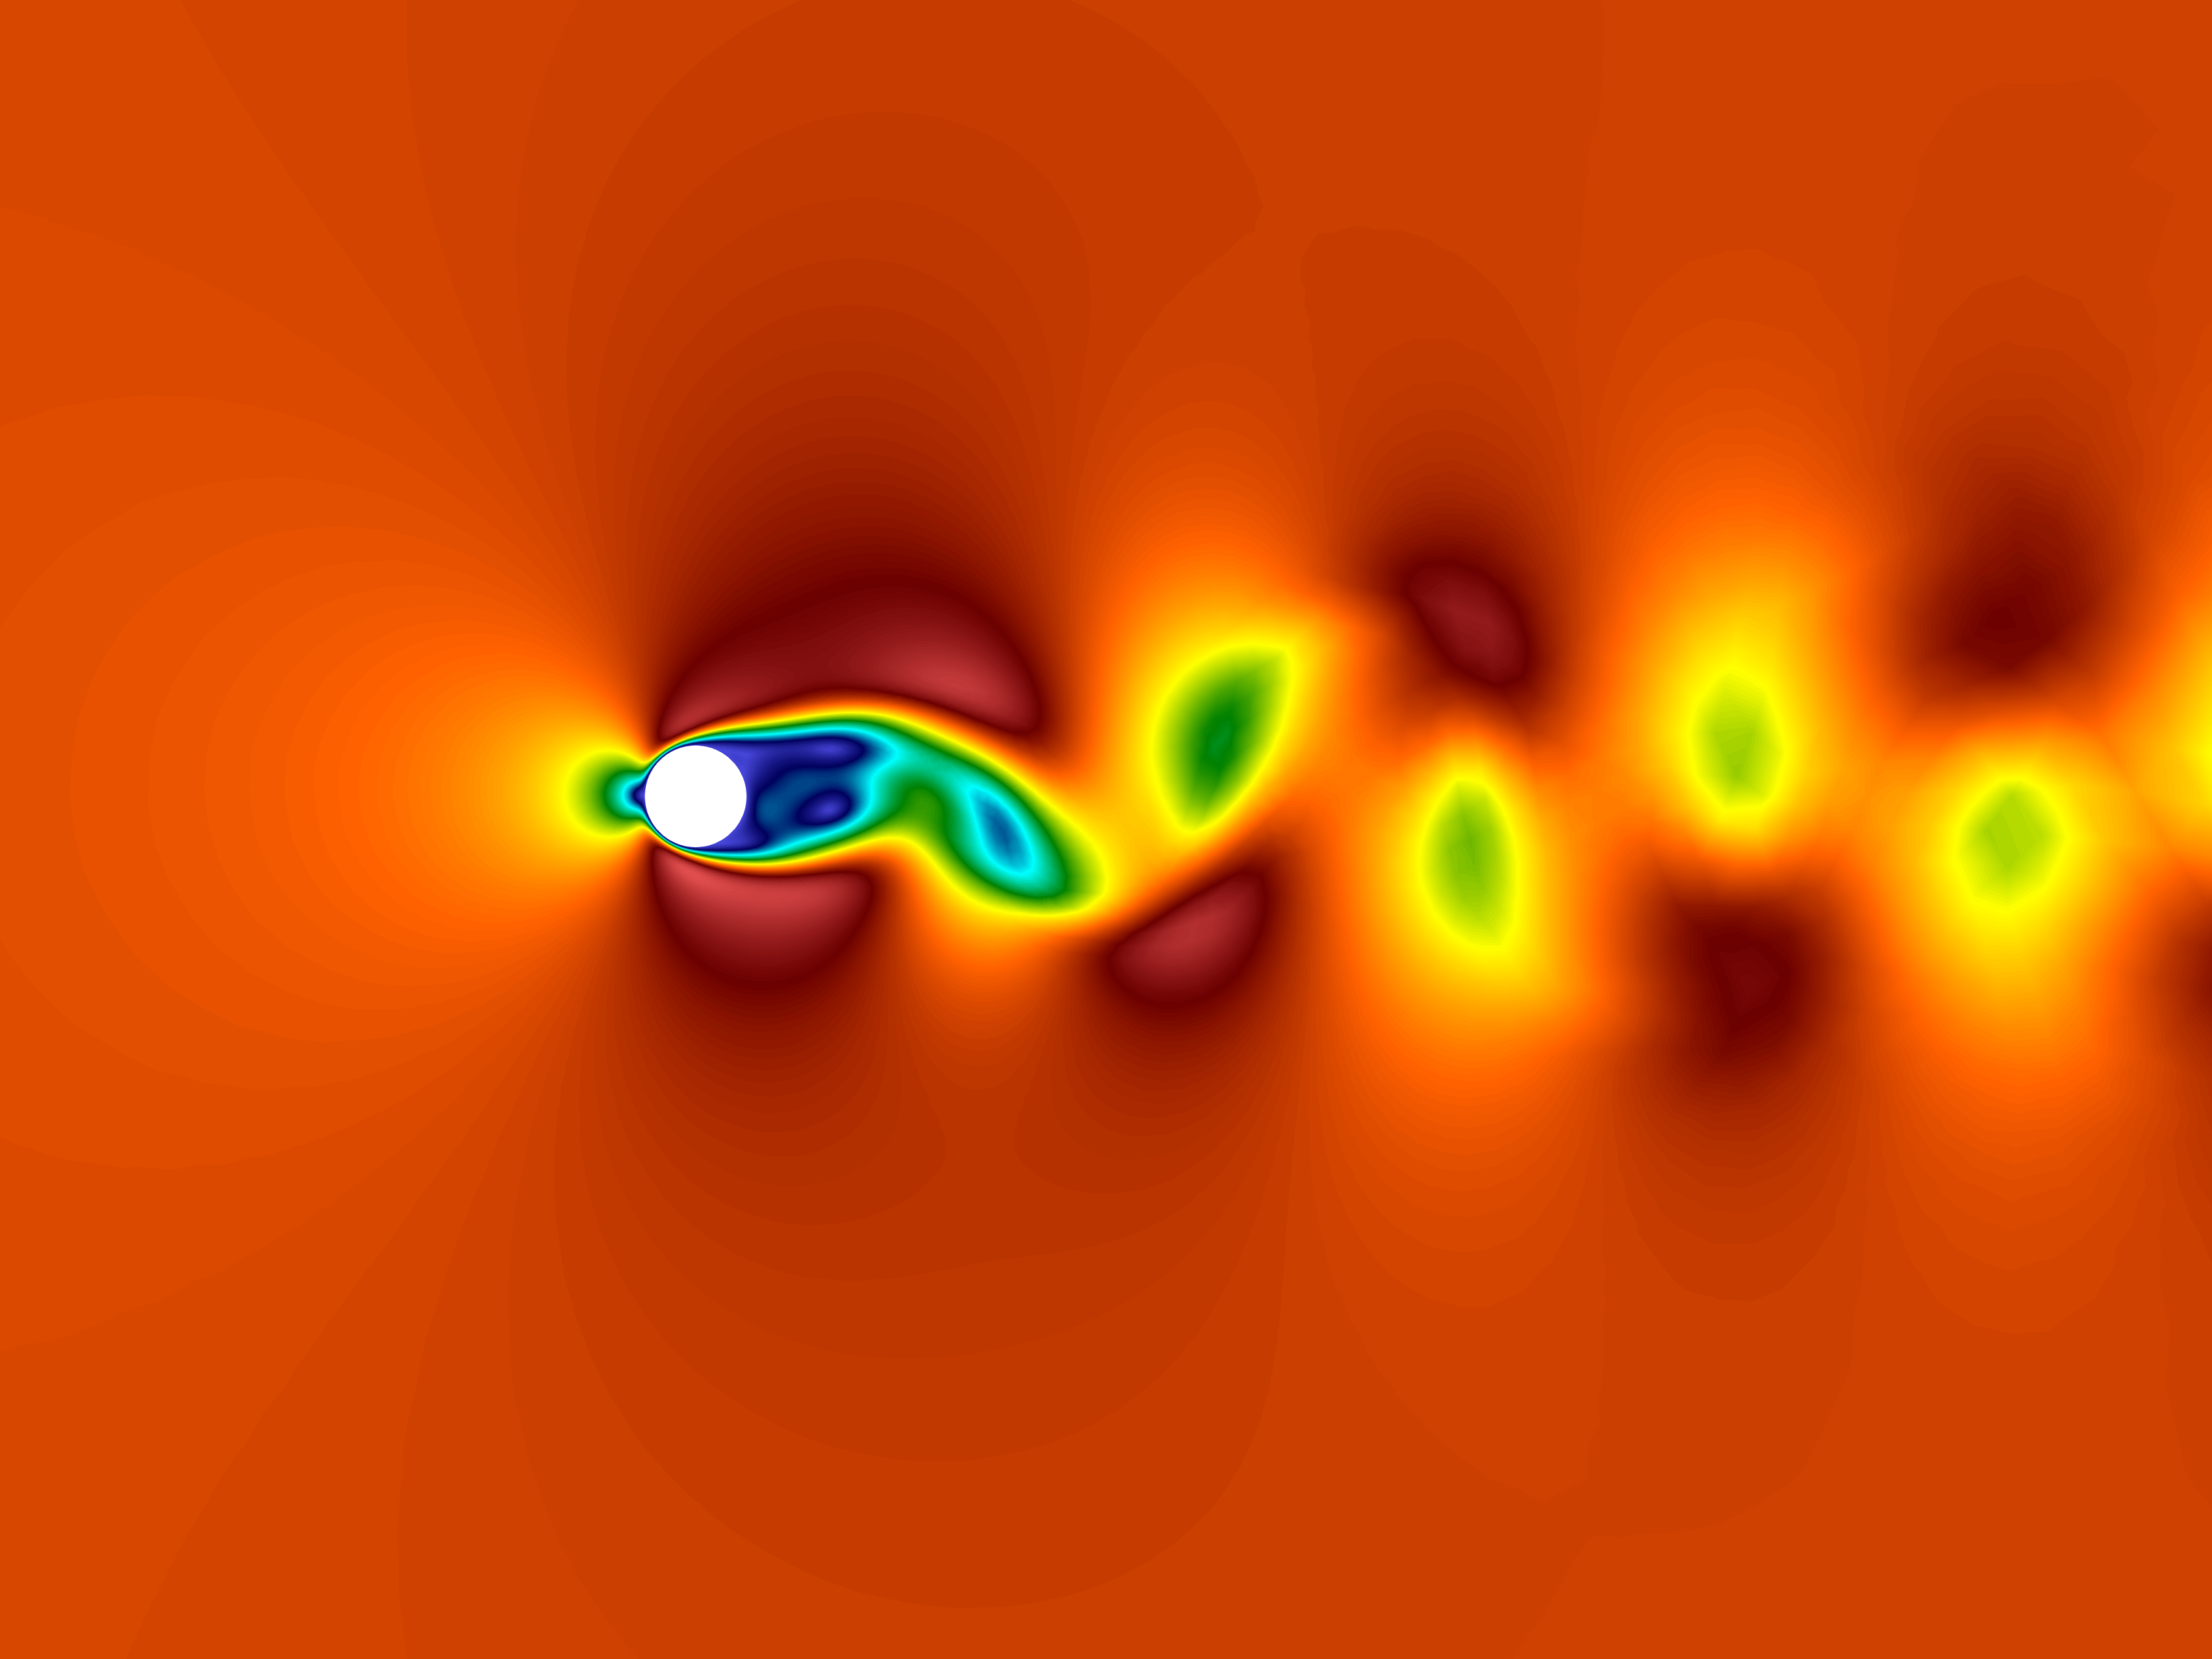
\includegraphics[scale=0.15,trim=5cm 5cm 5cm 6cm, clip=true]{Imagens/Cap2/cilindro_vel2030.pdf}} \\
	\subfloat[$nT + nT/3$]{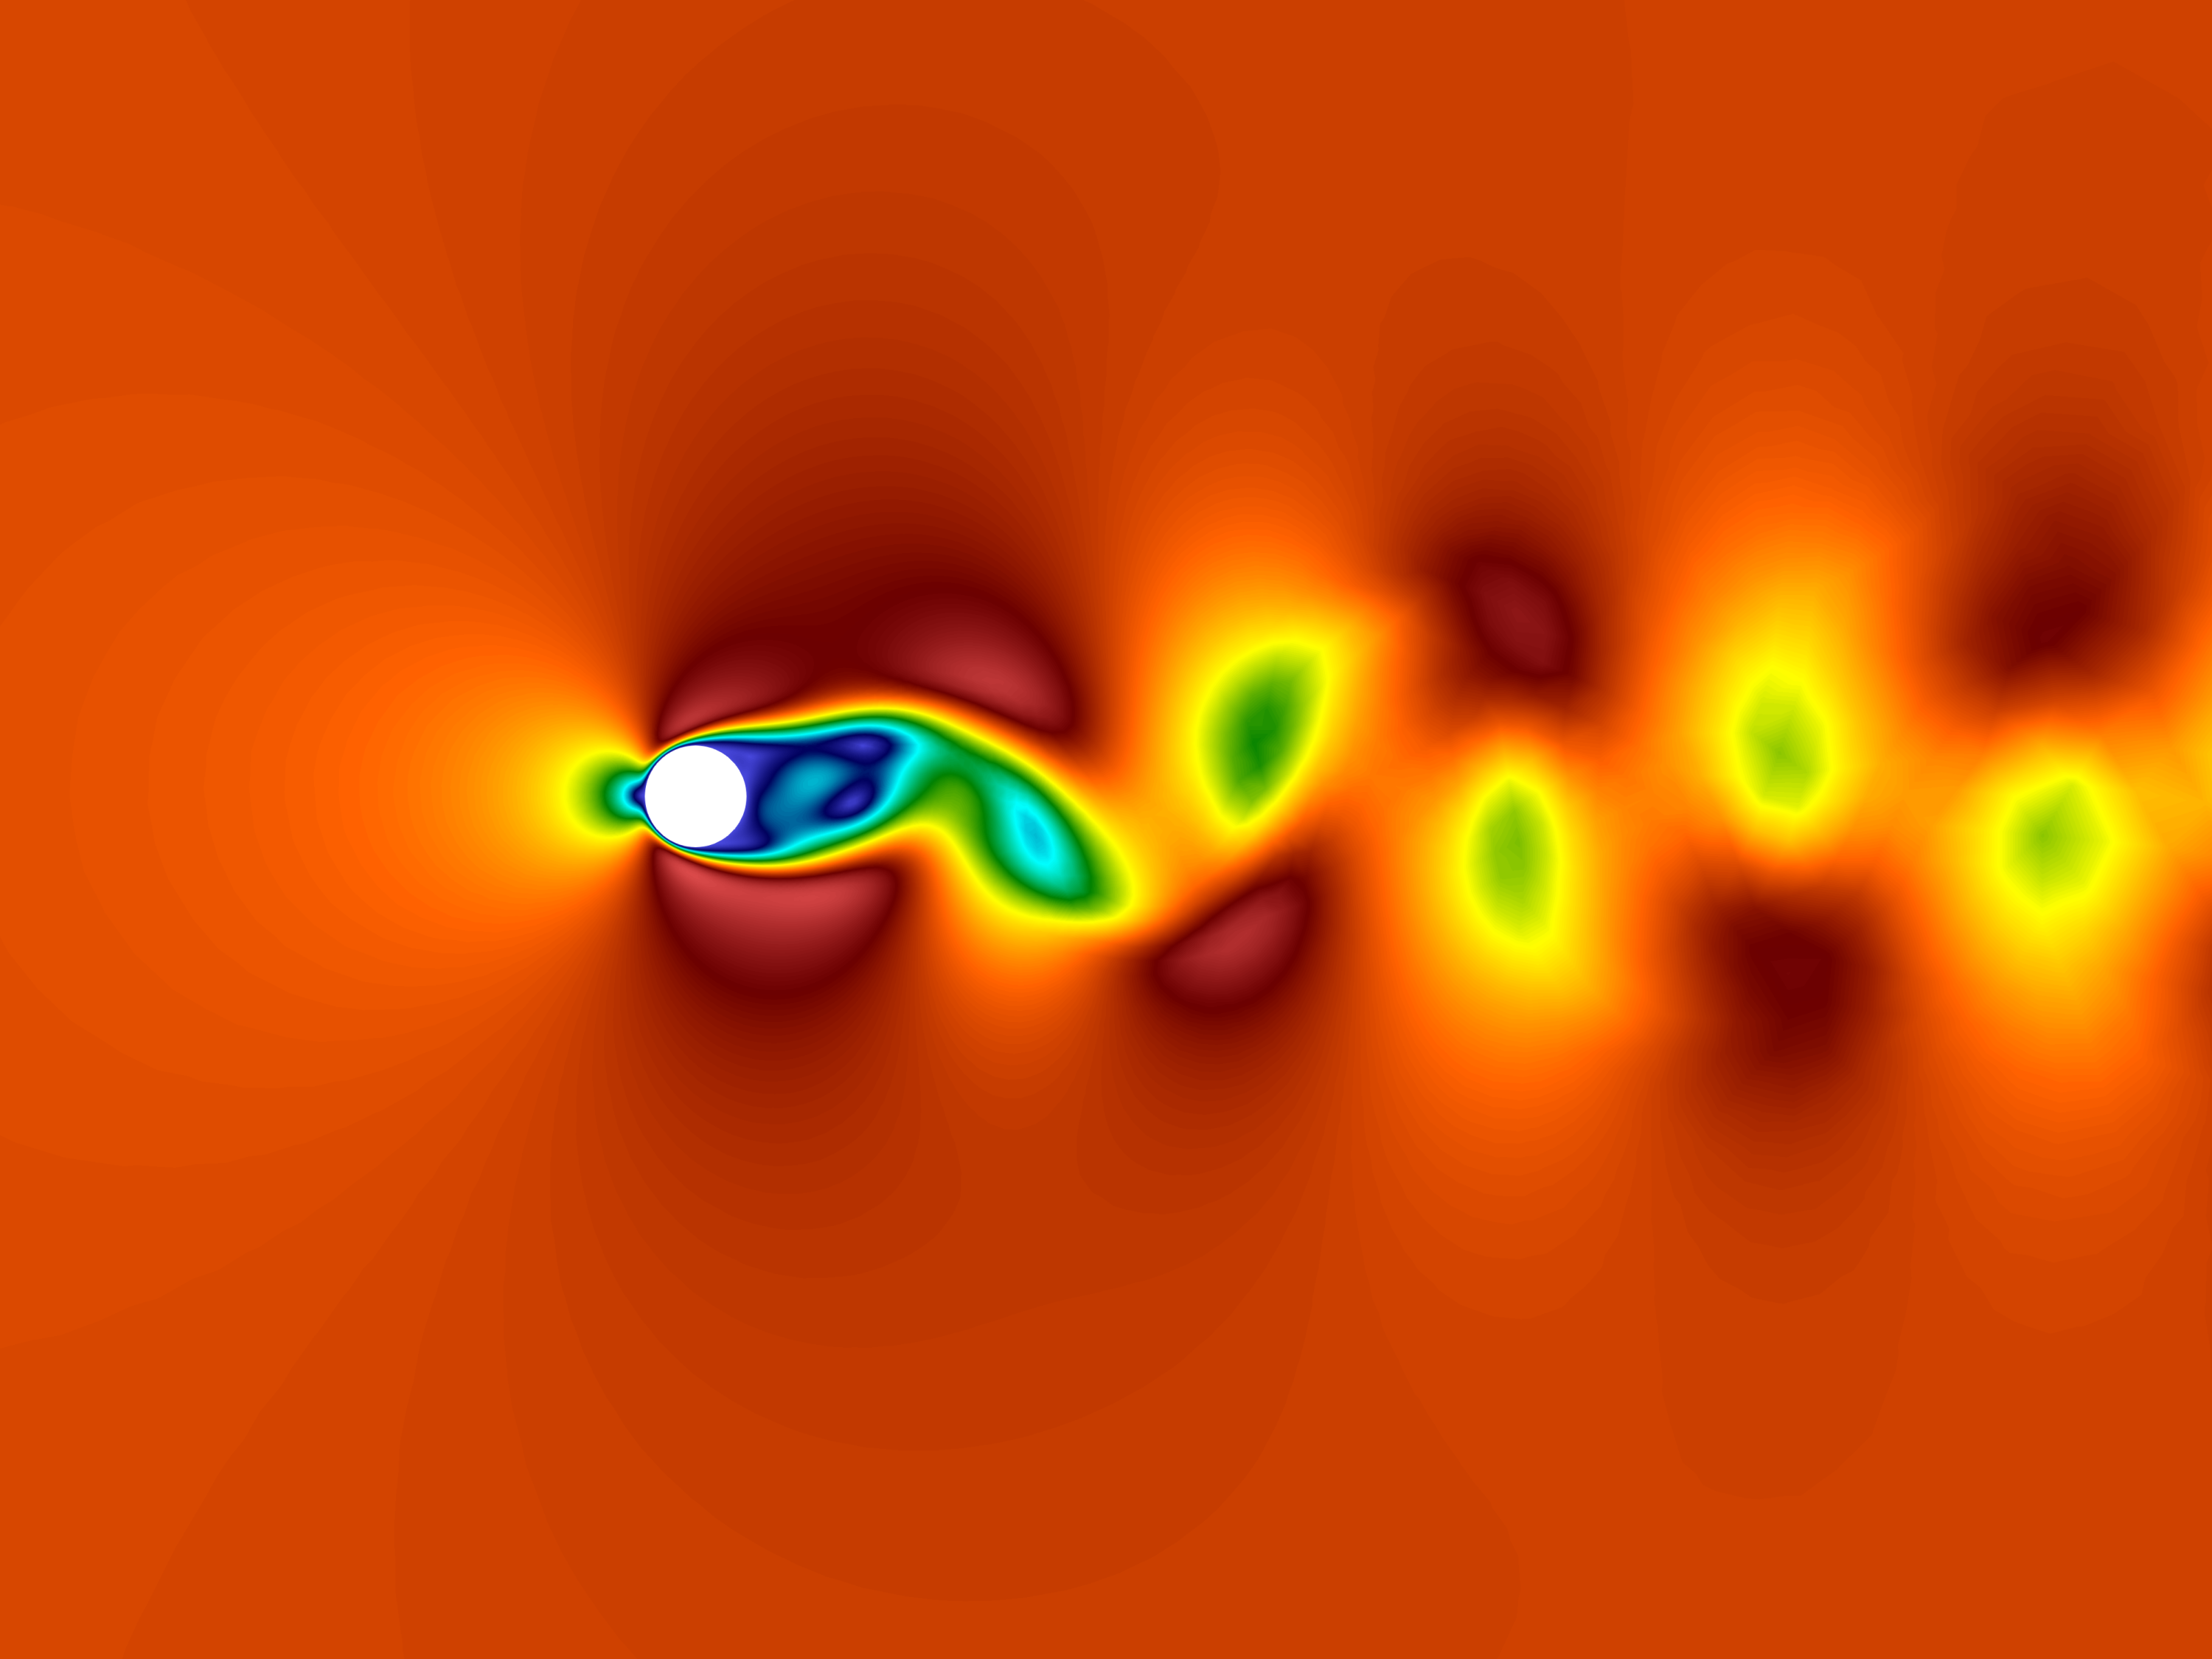
\includegraphics[scale=0.15,trim=5cm 5cm 5cm 6cm, clip=true]{Imagens/Cap2/cilindro_vel2040.pdf}} \
	\subfloat[$nT + nT/2$]{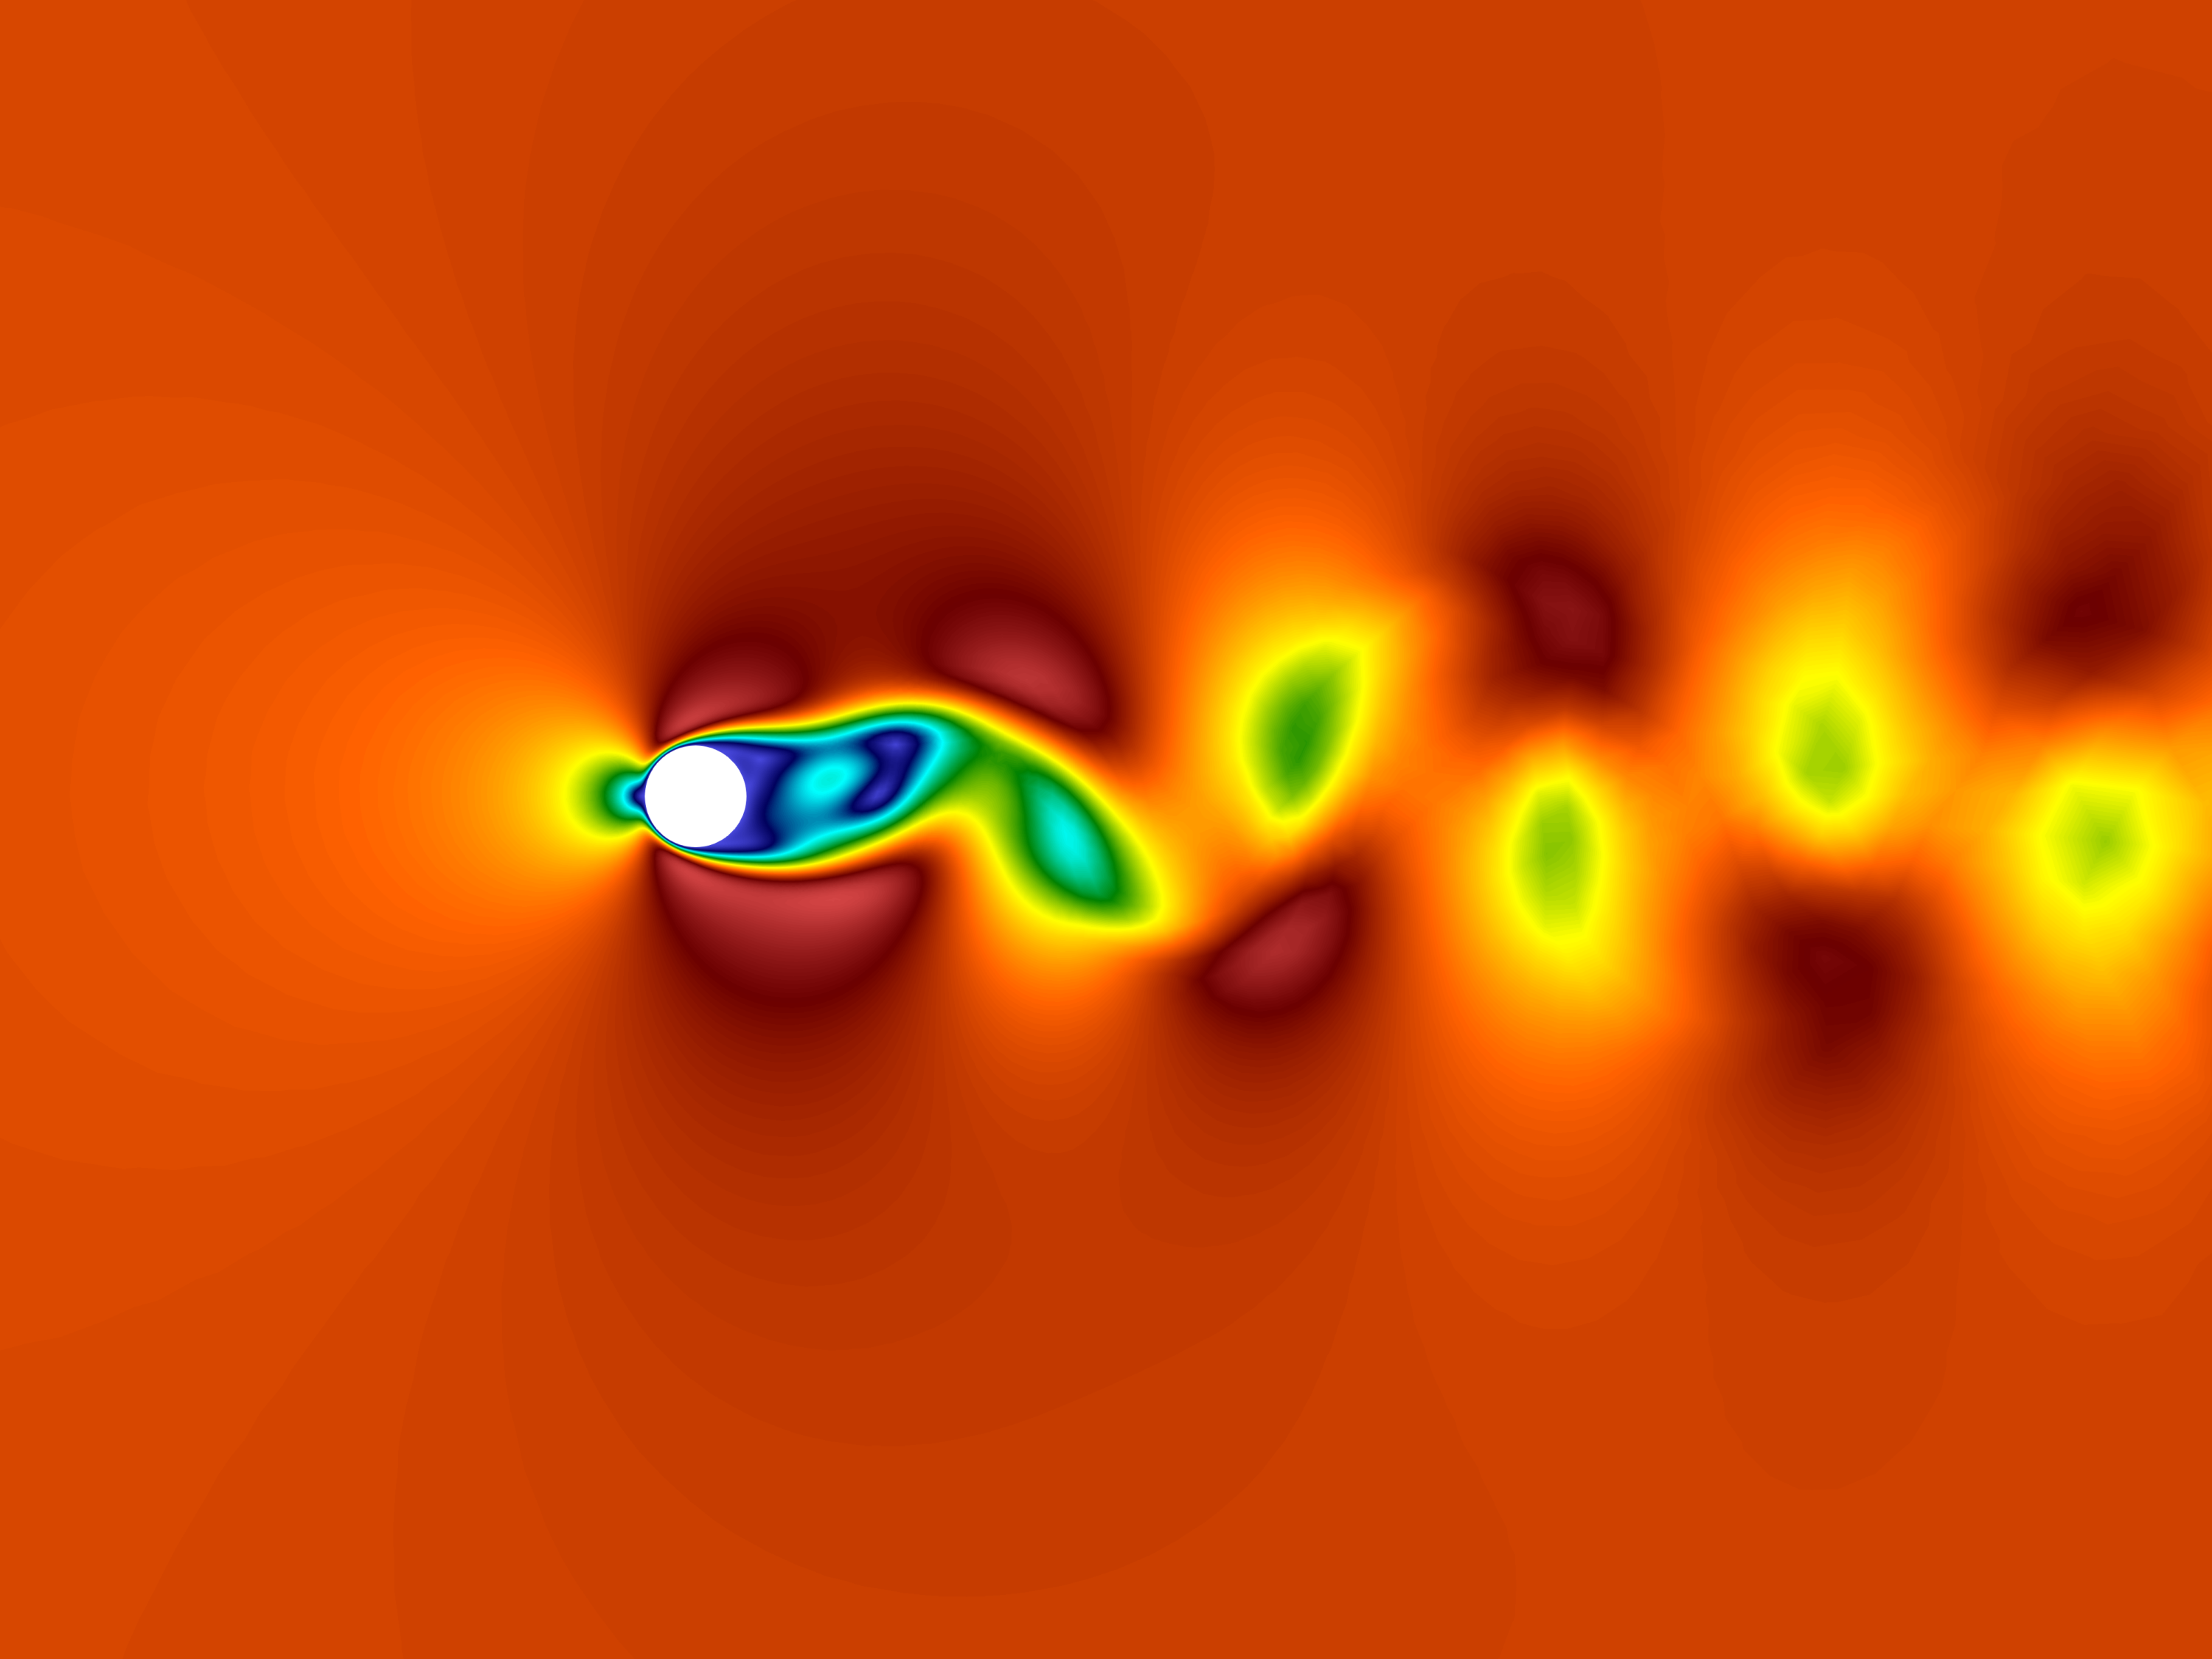
\includegraphics[scale=0.15,trim=5cm 5cm 5cm 6cm, clip=true]{Imagens/Cap2/cilindro_vel2050.pdf}} \\
	\subfloat[$nT + n2T/3$]{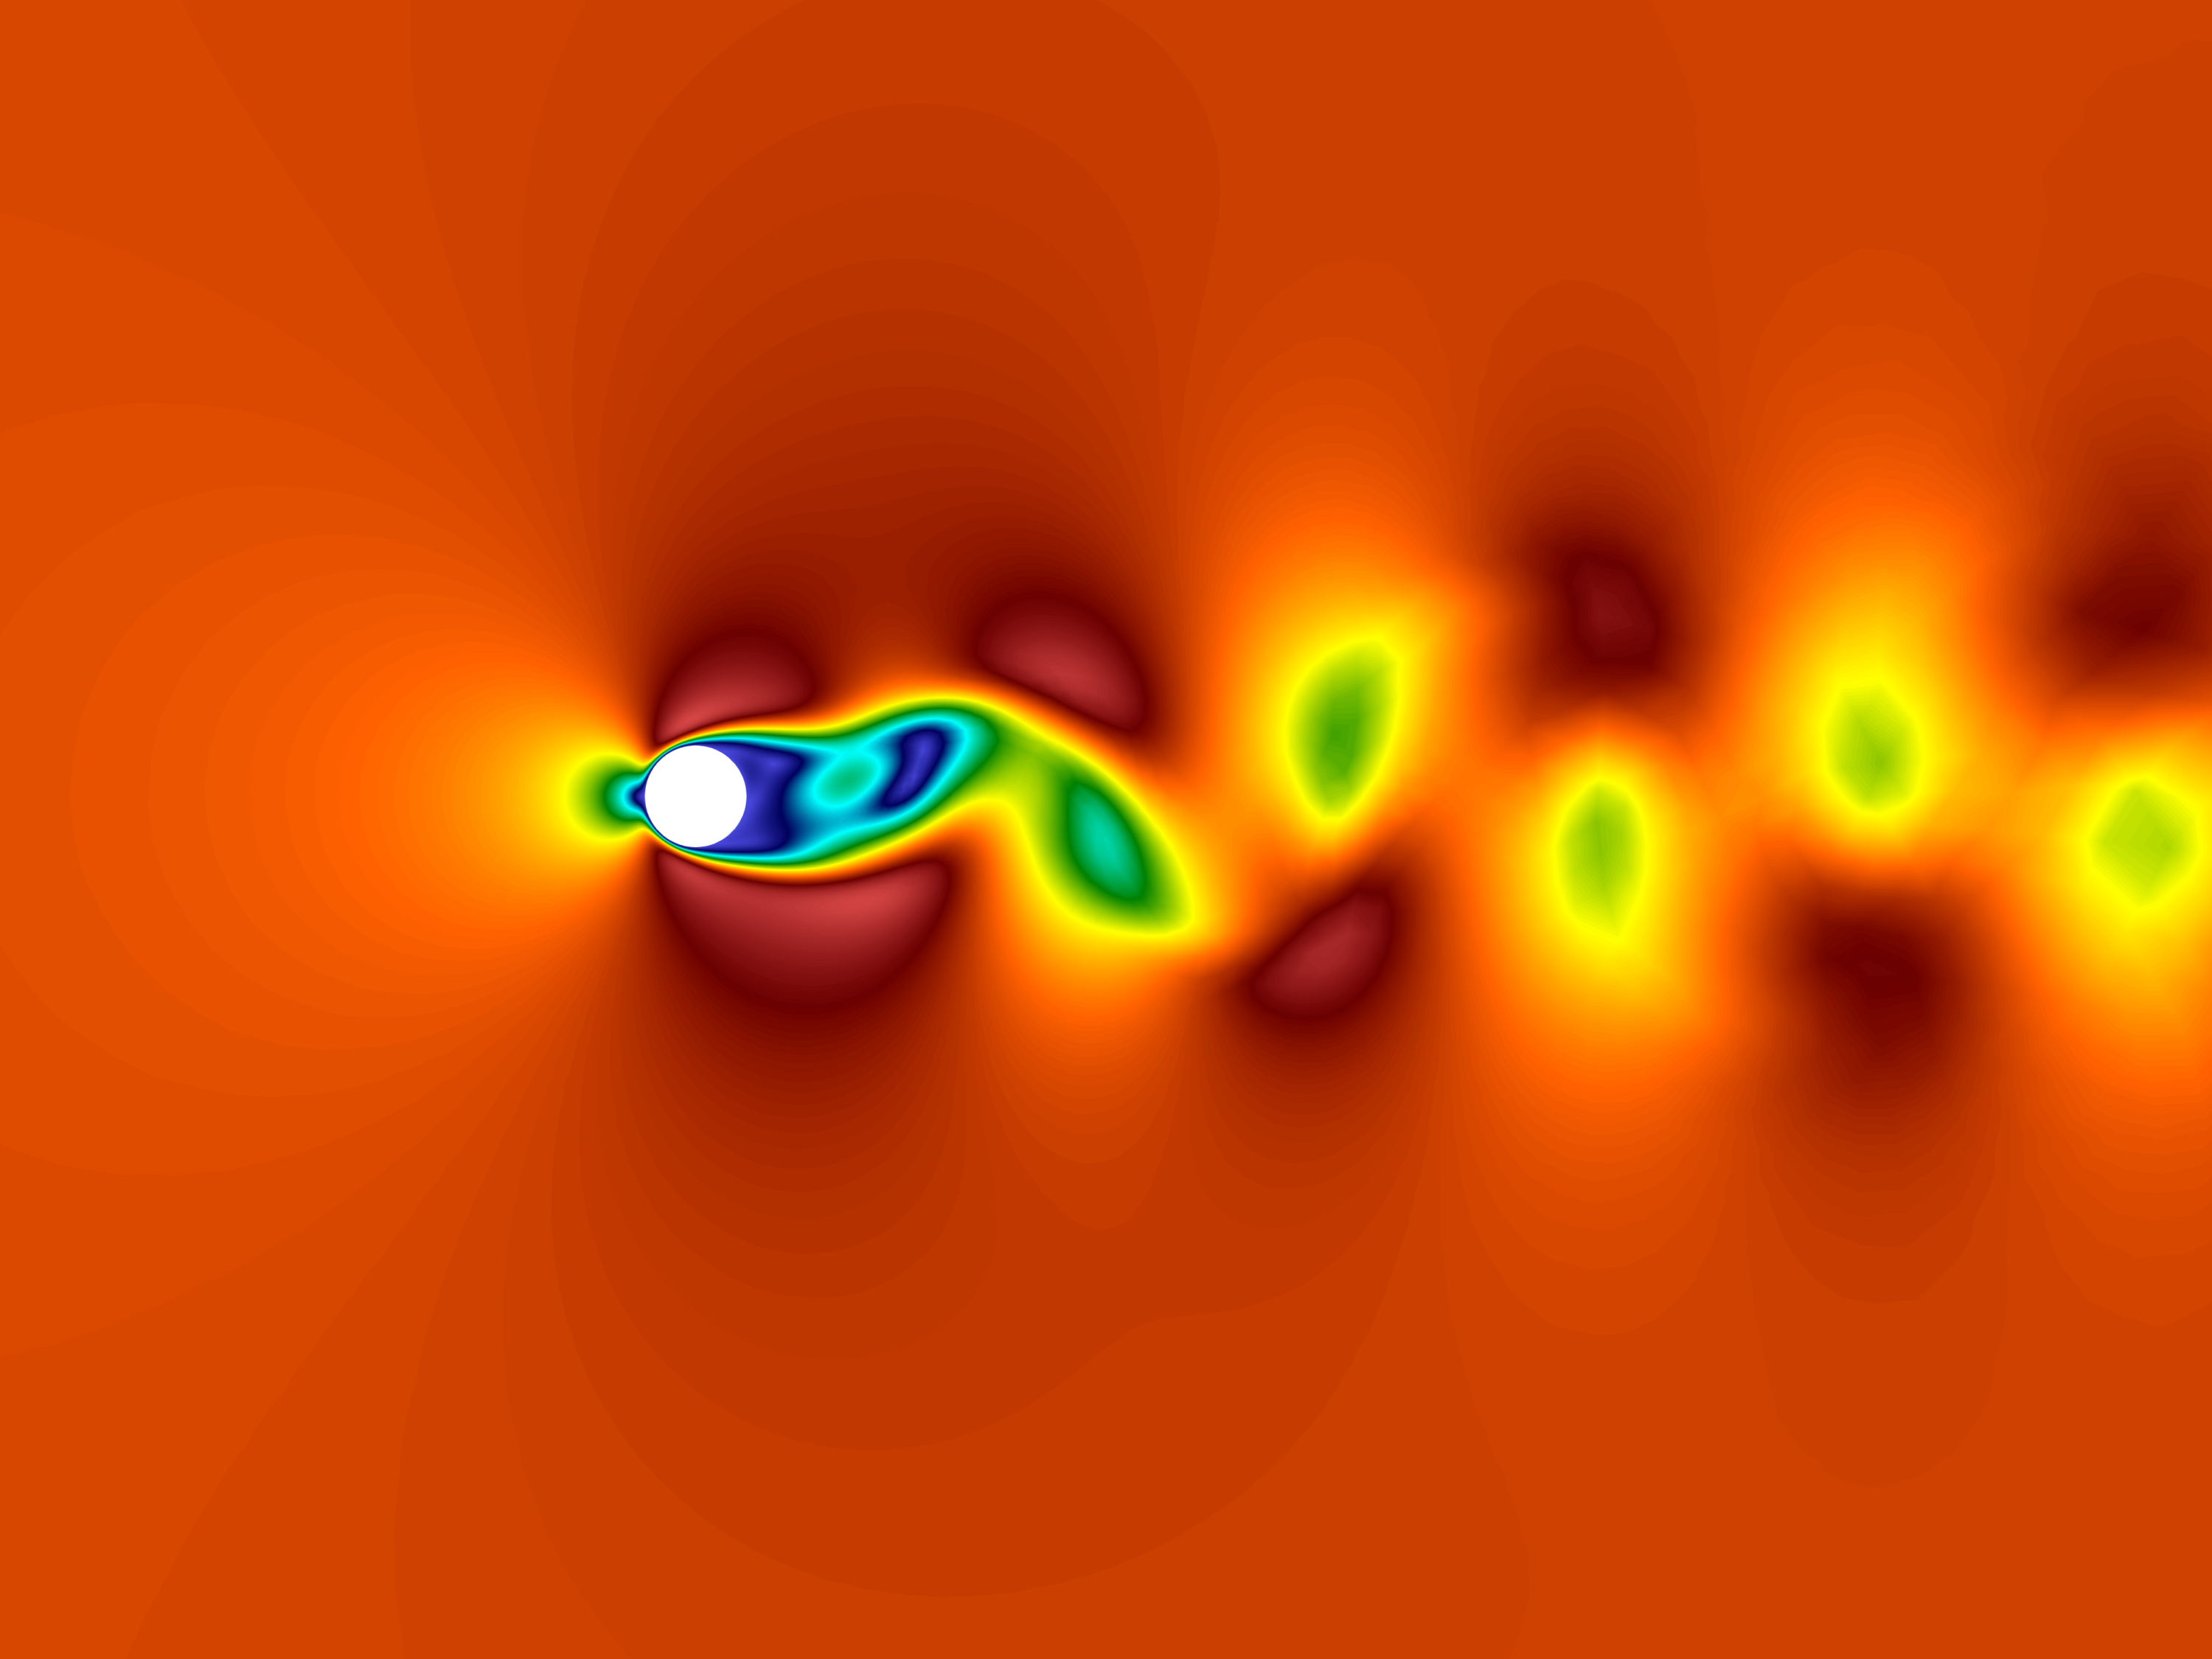
\includegraphics[scale=0.15,trim=5cm 5cm 5cm 6cm, clip=true]{Imagens/Cap2/cilindro_vel2060.pdf}} \
	\subfloat[$nT + n5T/6$]{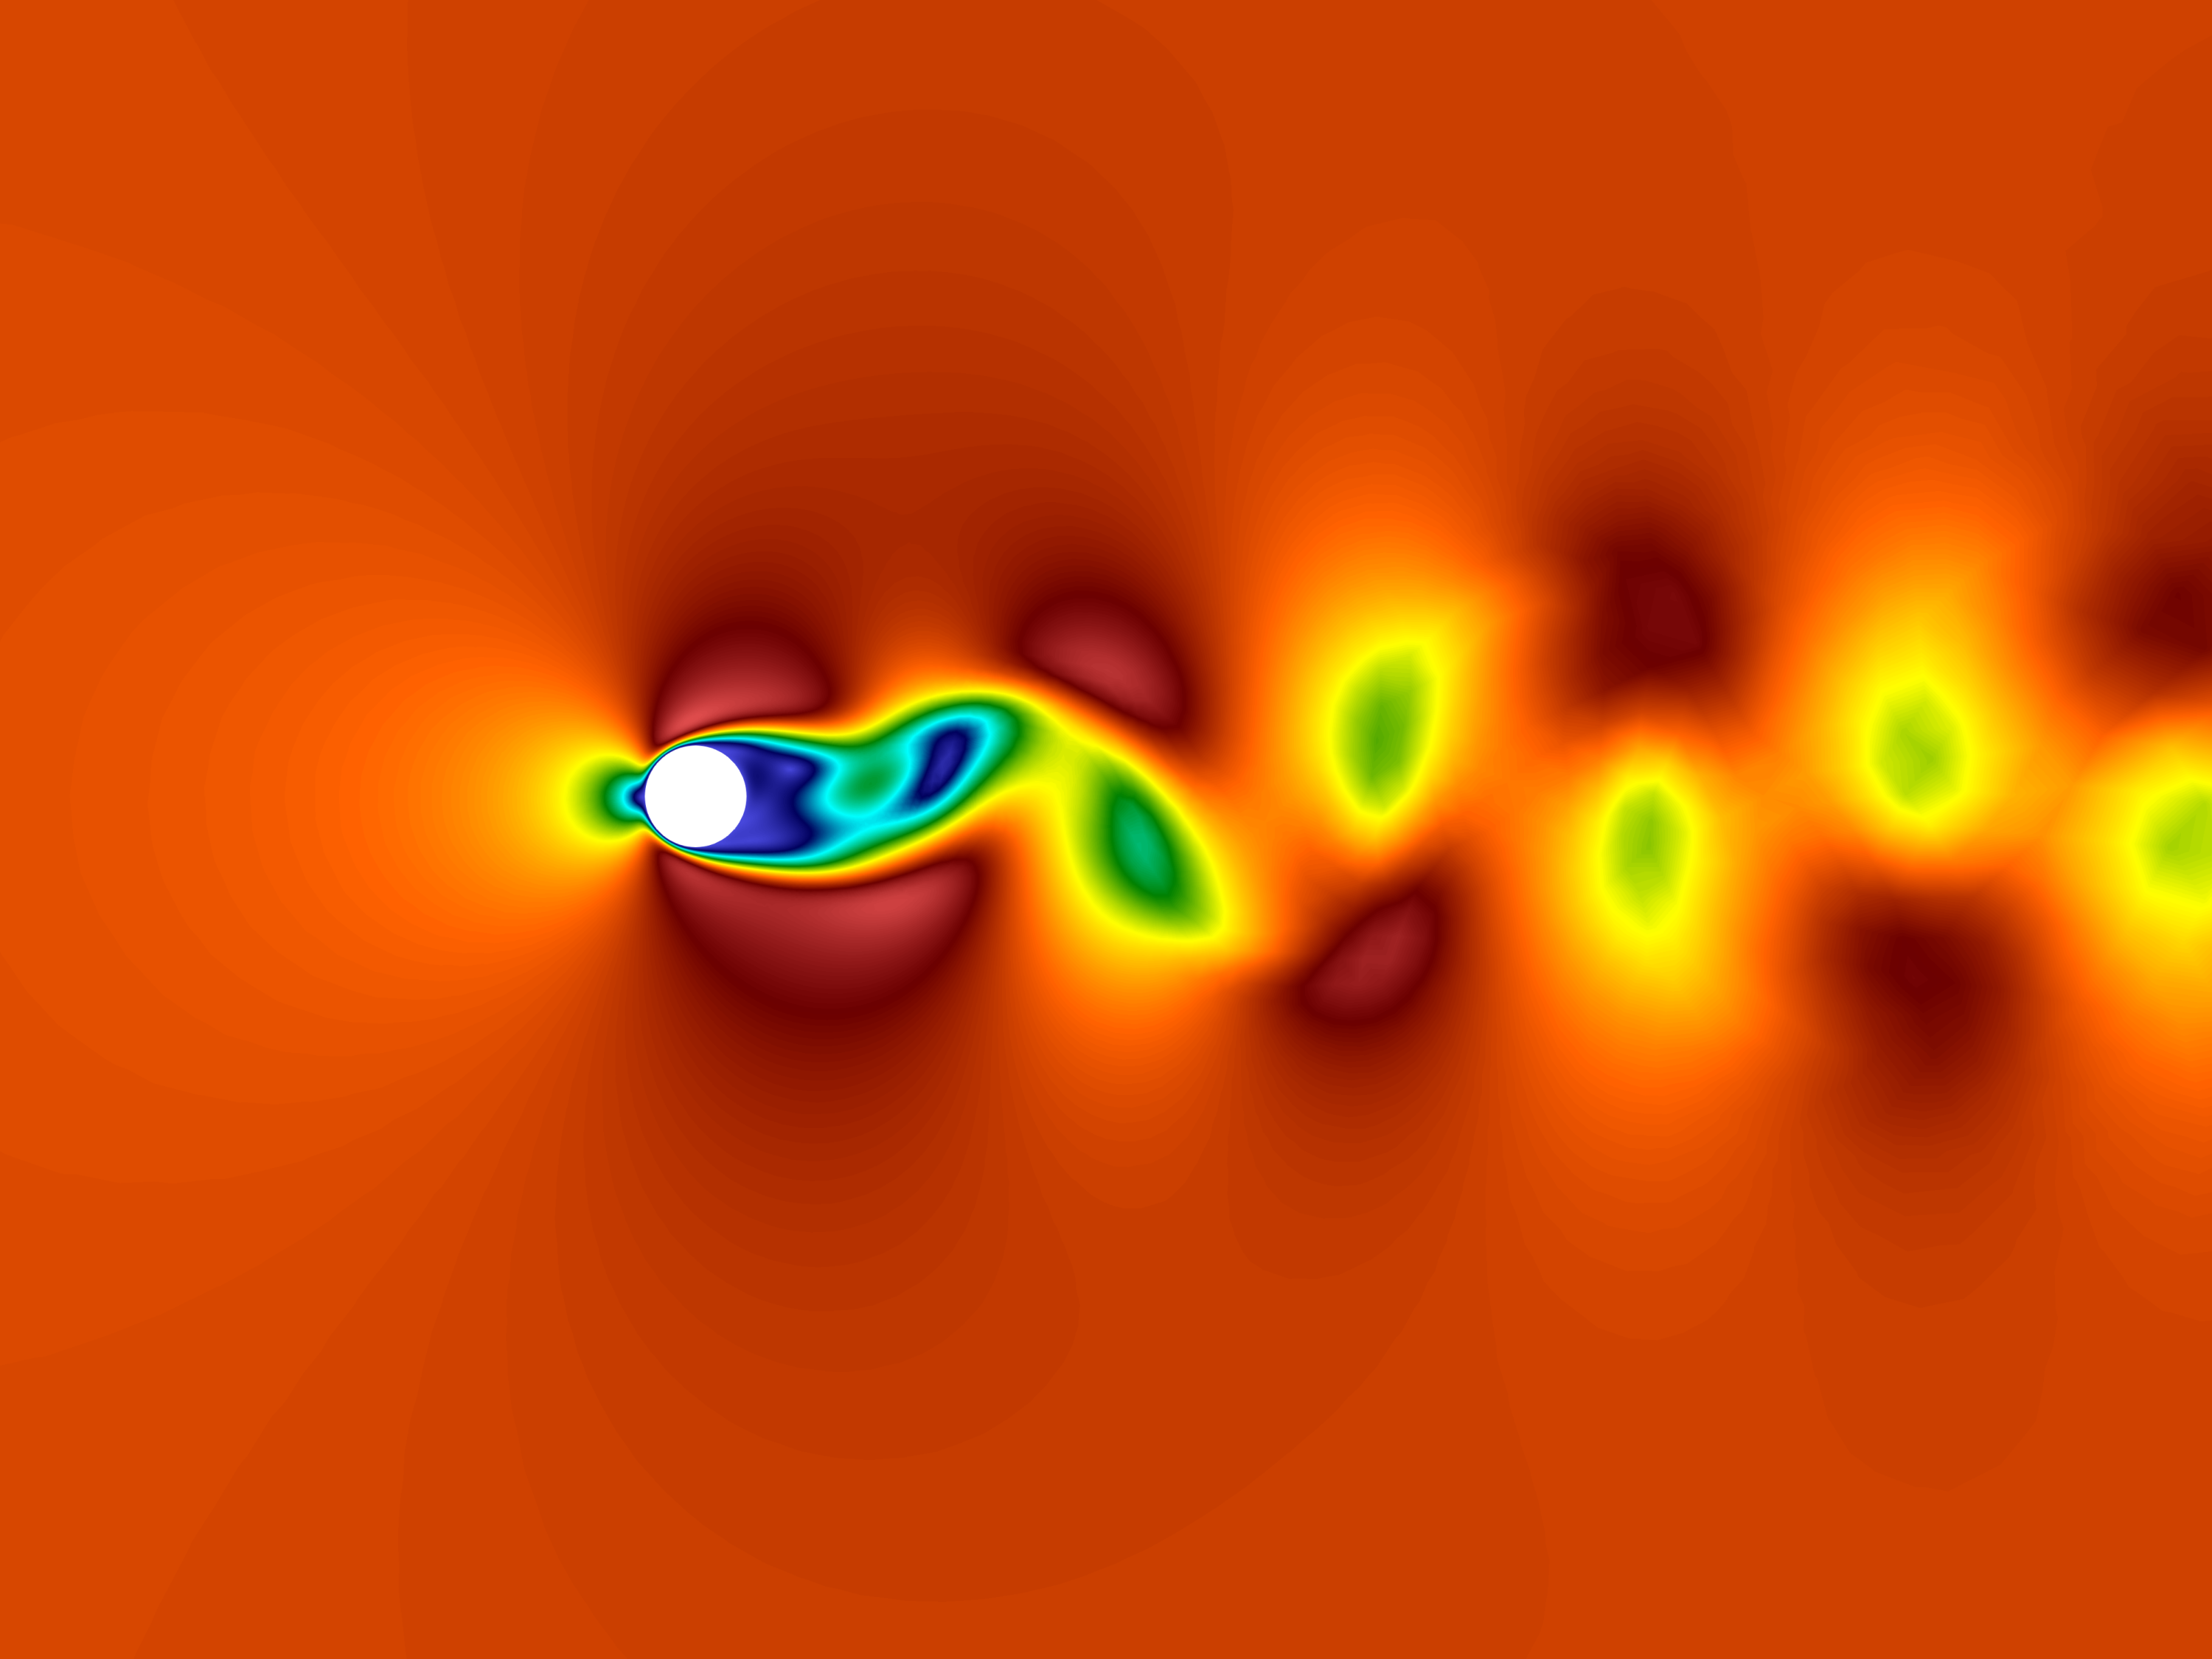
\includegraphics[scale=0.15,trim=5cm 5cm 5cm 6cm, clip=true]{Imagens/Cap2/cilindro_vel2070.pdf}} \\
	{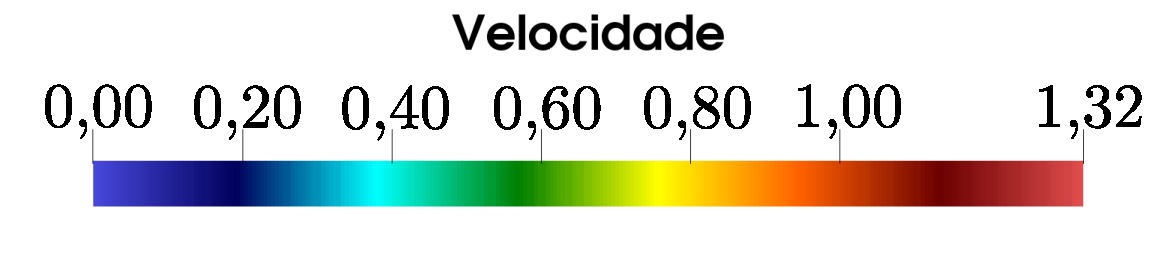
\includegraphics[trim=0cm 0.2cm 0cm 0cm,clip=true,scale=0.3]{Imagens/Cap2/cilindro_legendaVel.pdf}}
	\label{fig:cilindro_camposVel}
	\legend{Fonte: Elaborada pela autora}
\end{figure}

\begin{figure}[!htbp]
	\caption{Cilindro: Campos de pressão para $\Reynolds = 100$}
	\centering
	\subfloat[$nT$]{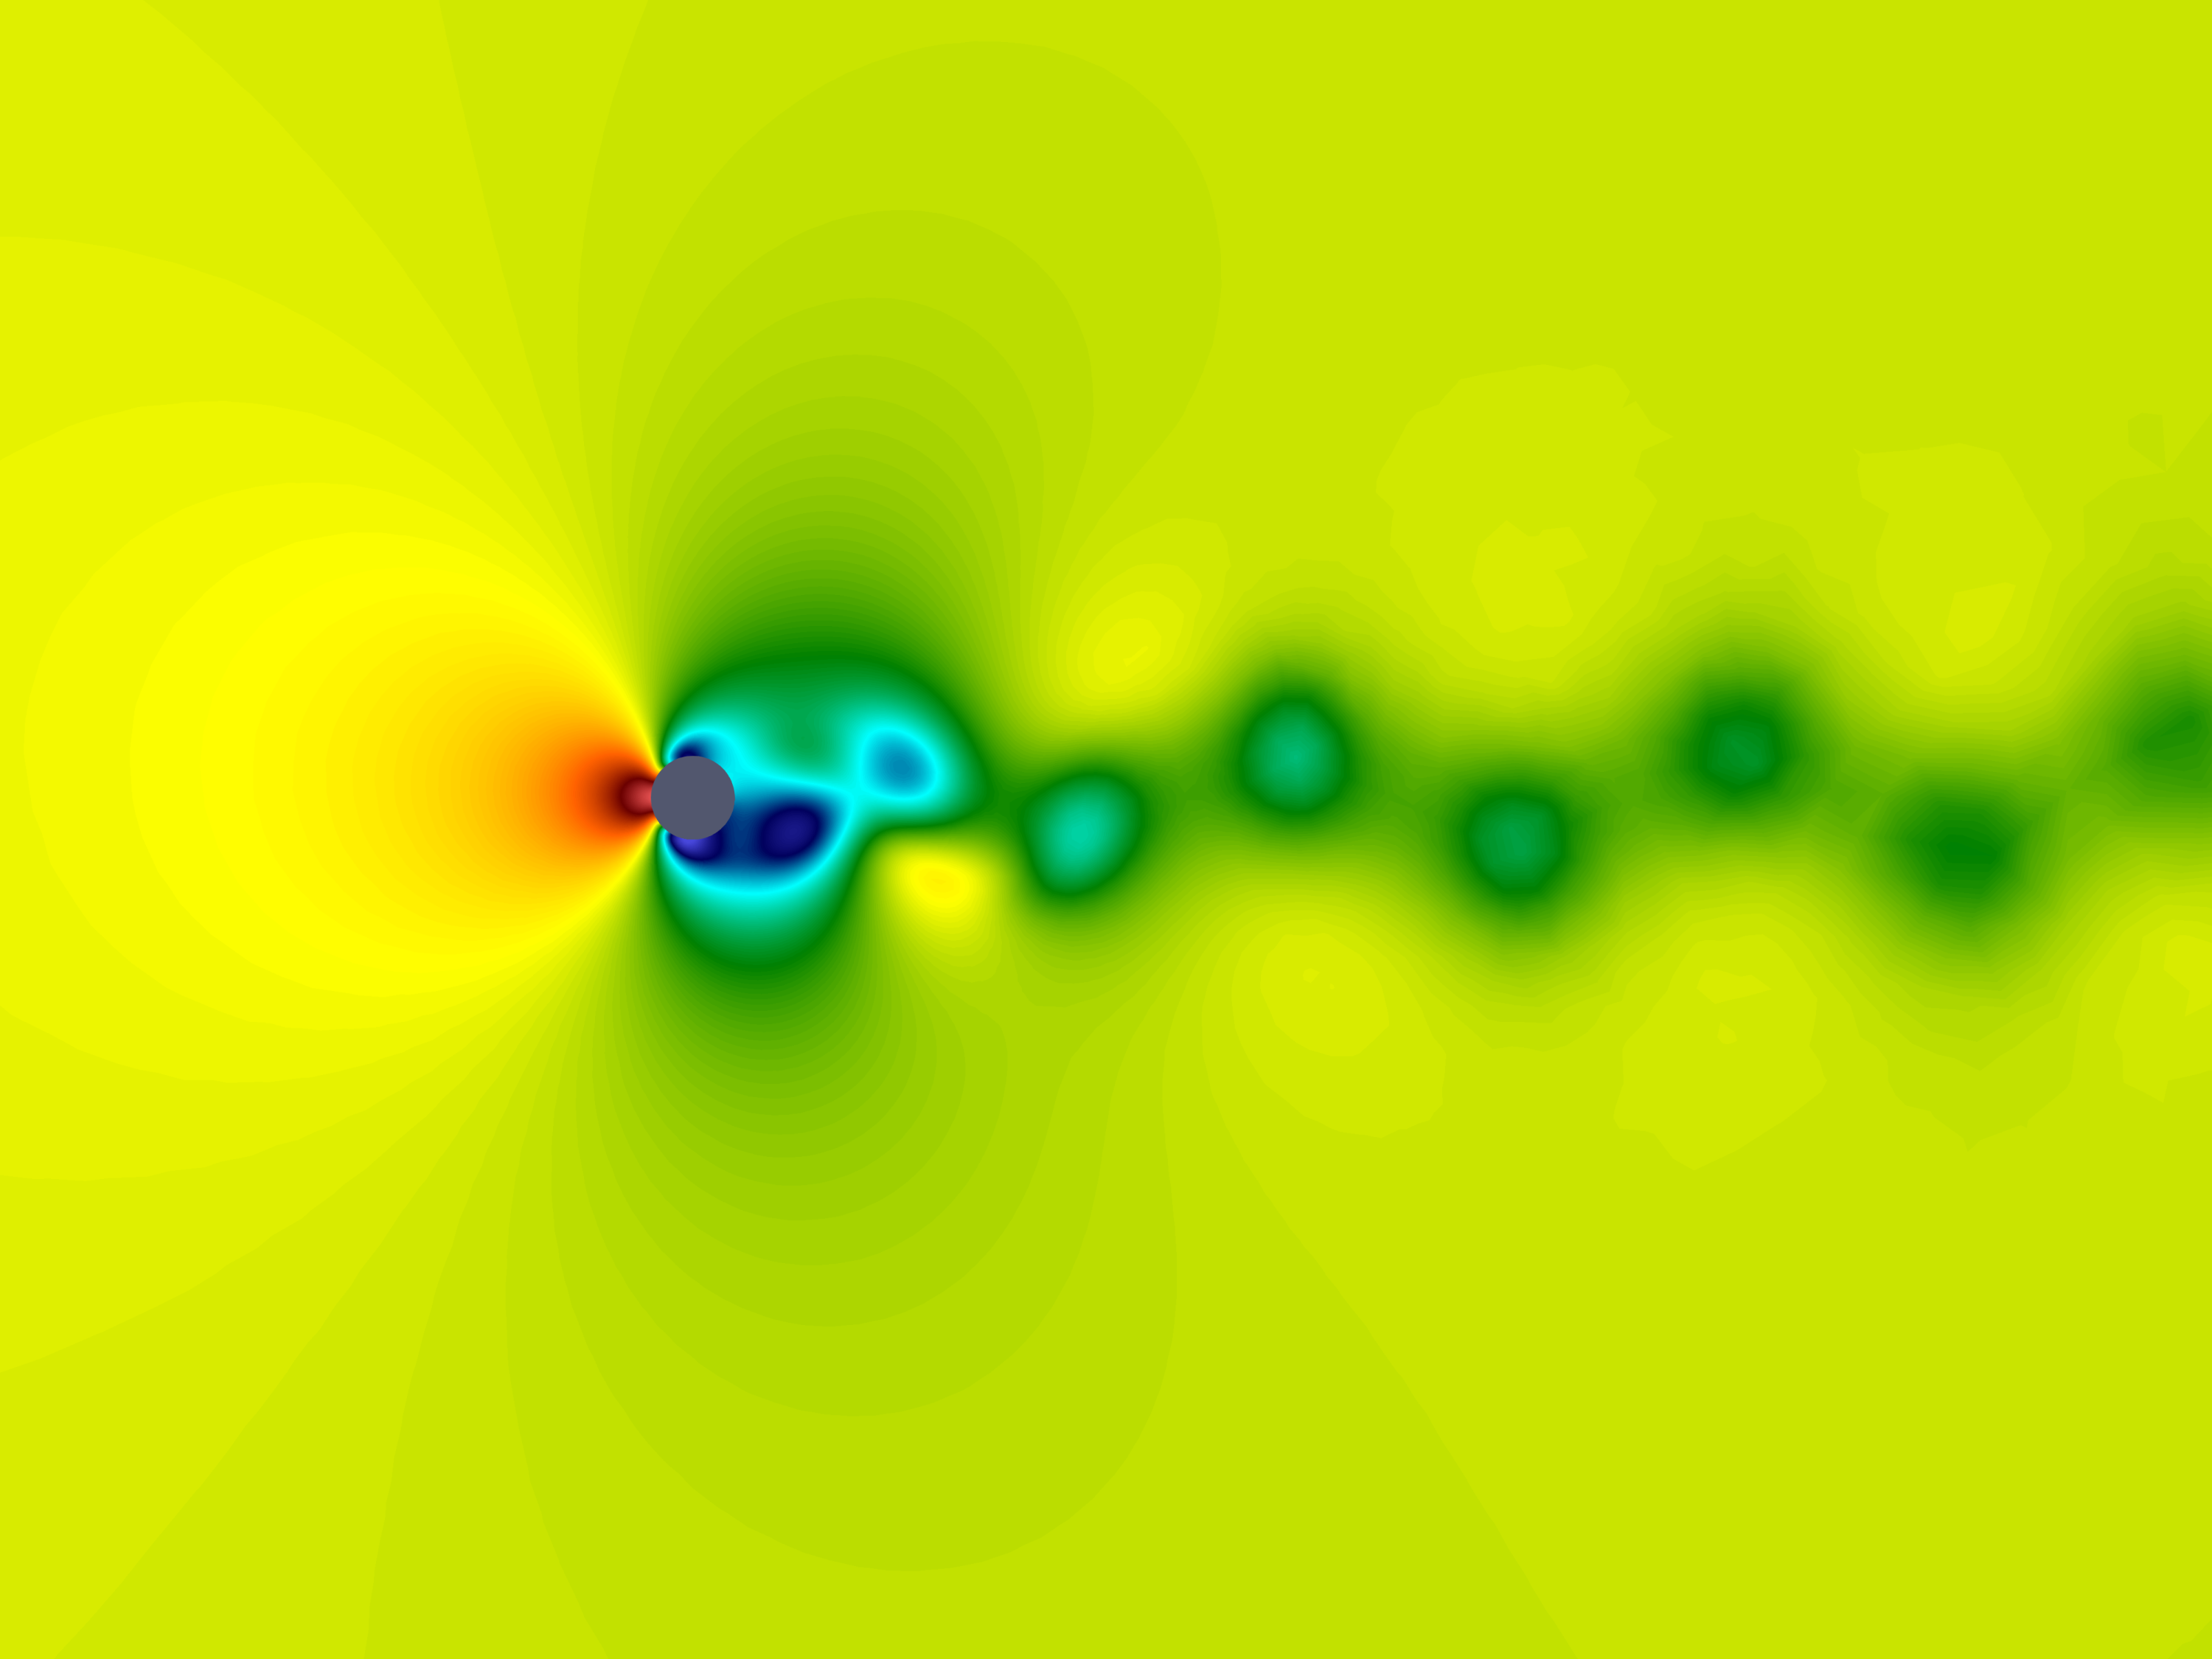
\includegraphics[scale=0.15,trim=5cm 5cm 5cm 6cm, clip=true]{Imagens/Cap2/cilindro_press2020.pdf}} \
	\subfloat[$nT + nT/6$]{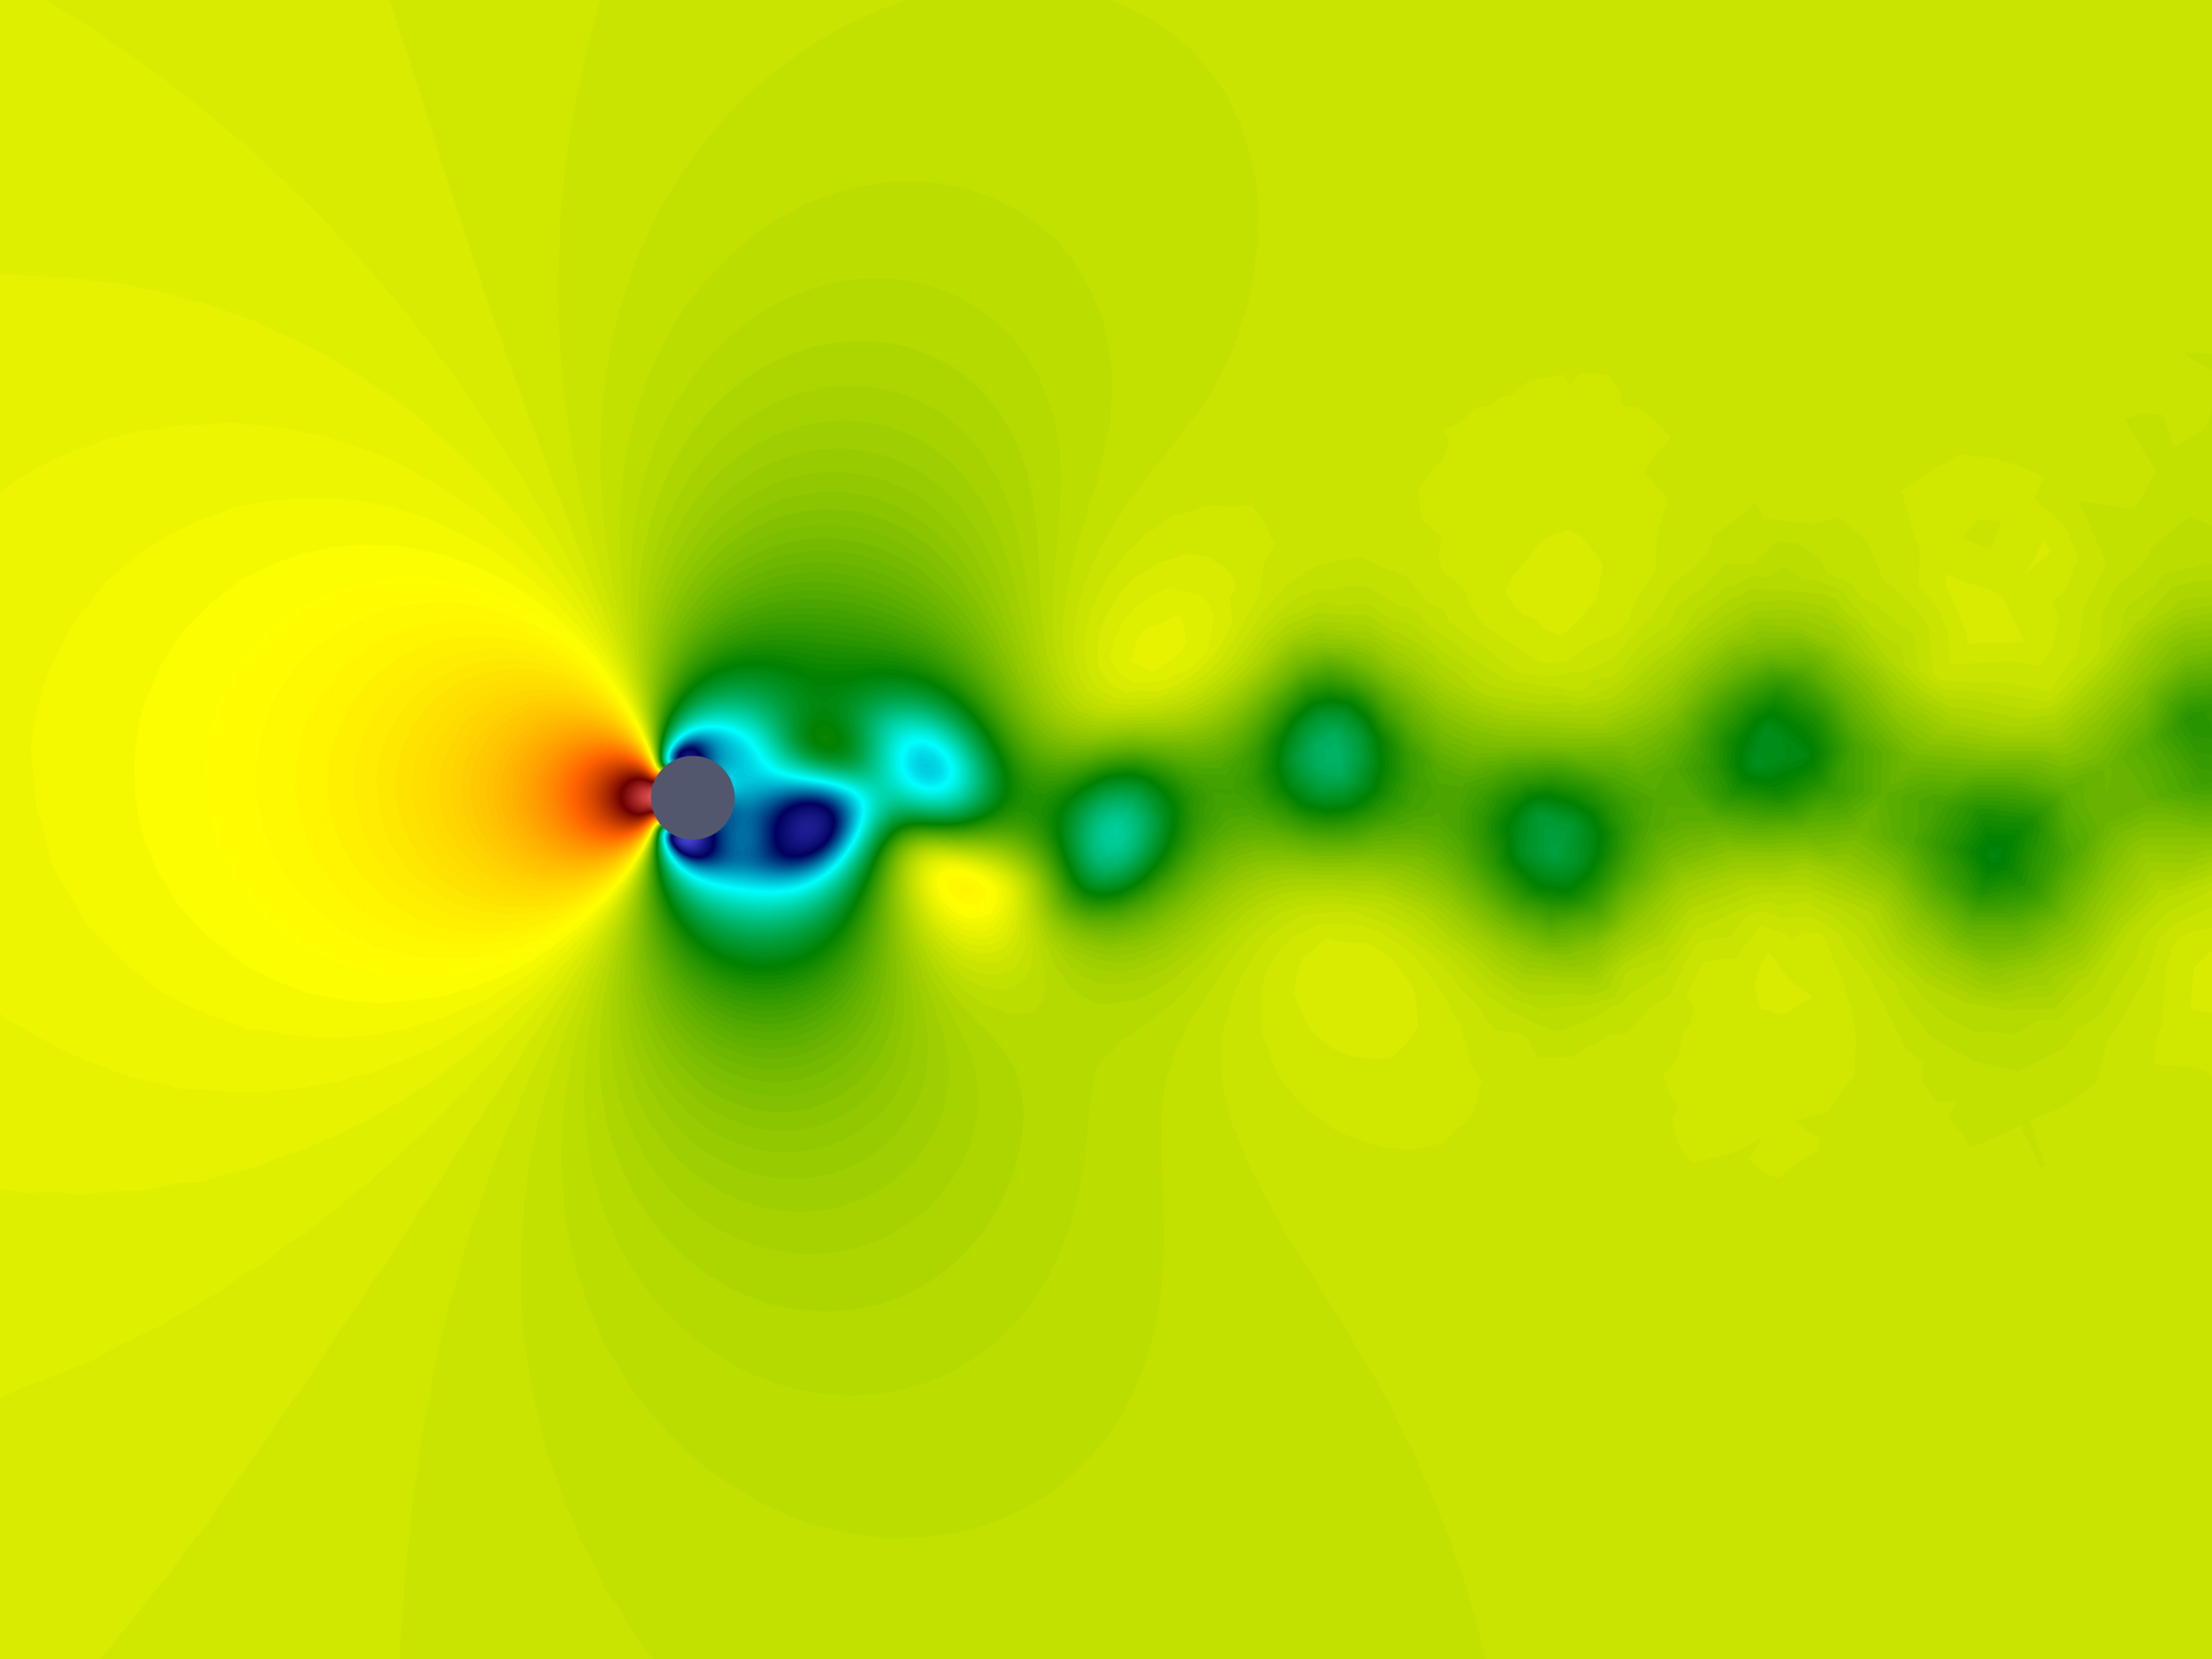
\includegraphics[scale=0.15,trim=5cm 5cm 5cm 6cm, clip=true]{Imagens/Cap2/cilindro_press2030.pdf}} \\
	\subfloat[$nT + nT/3$]{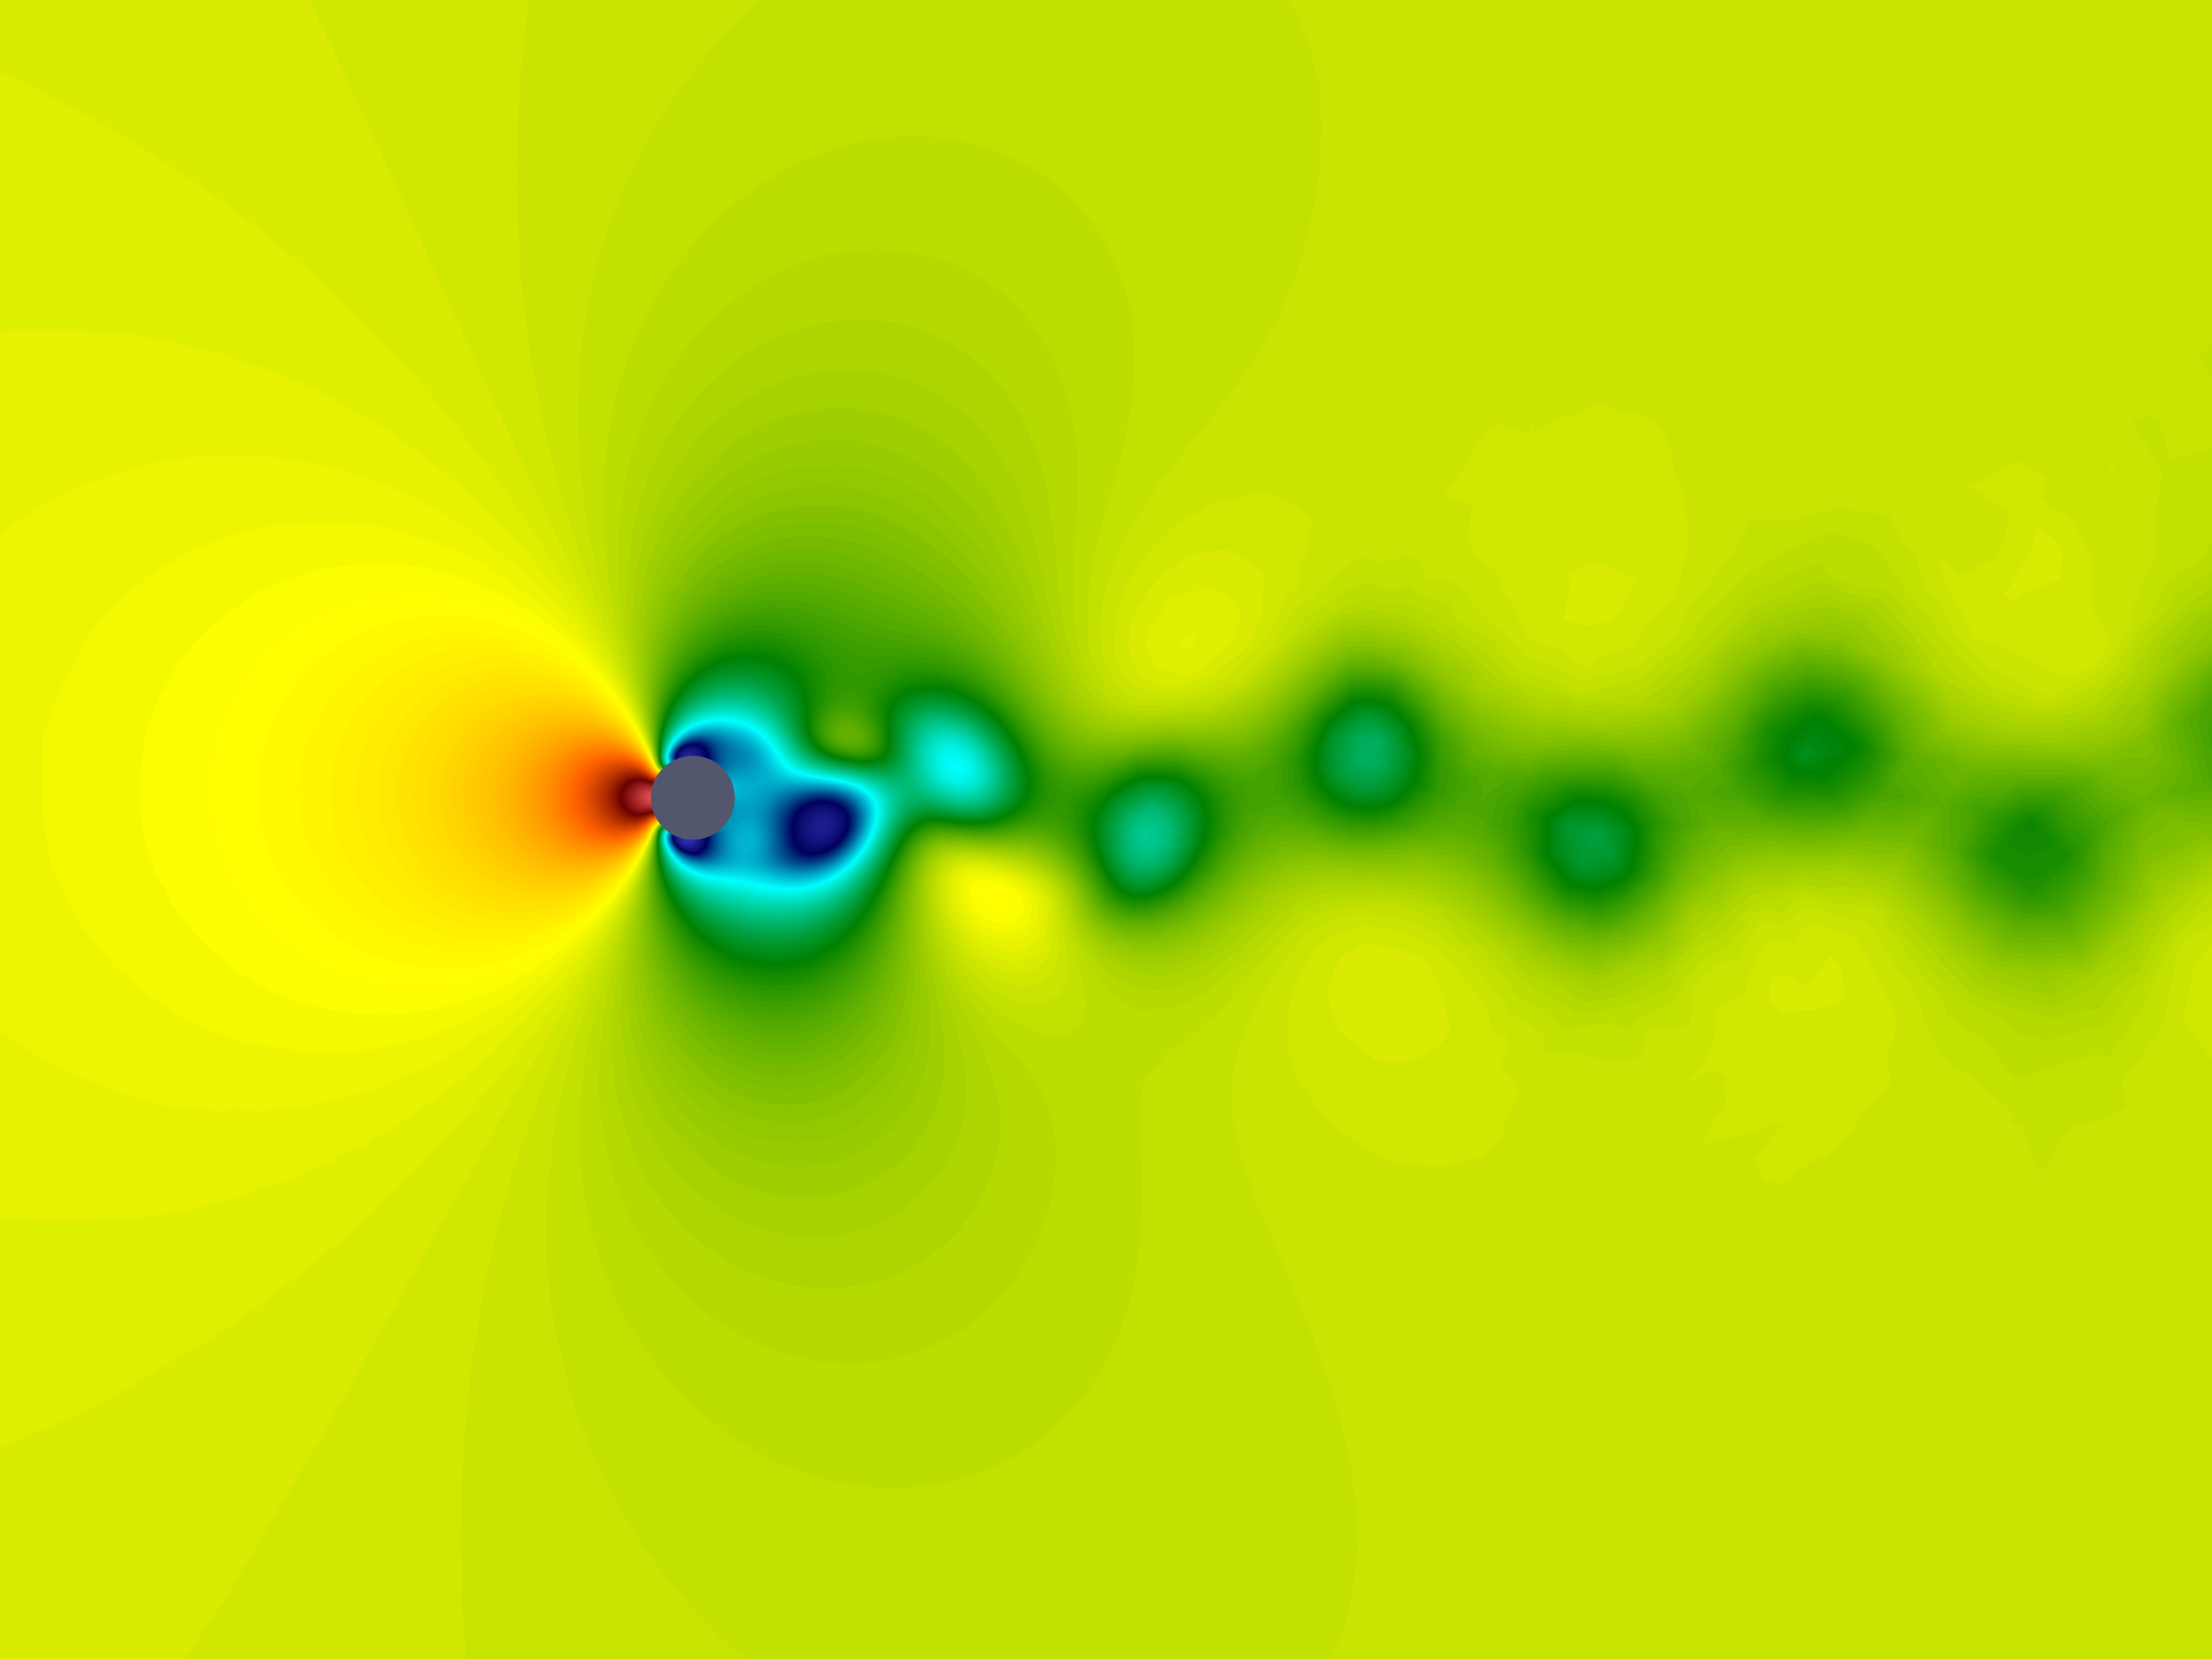
\includegraphics[scale=0.15,trim=5cm 5cm 5cm 6cm, clip=true]{Imagens/Cap2/cilindro_press2040.pdf}} \
	\subfloat[$nT + nT/2$]{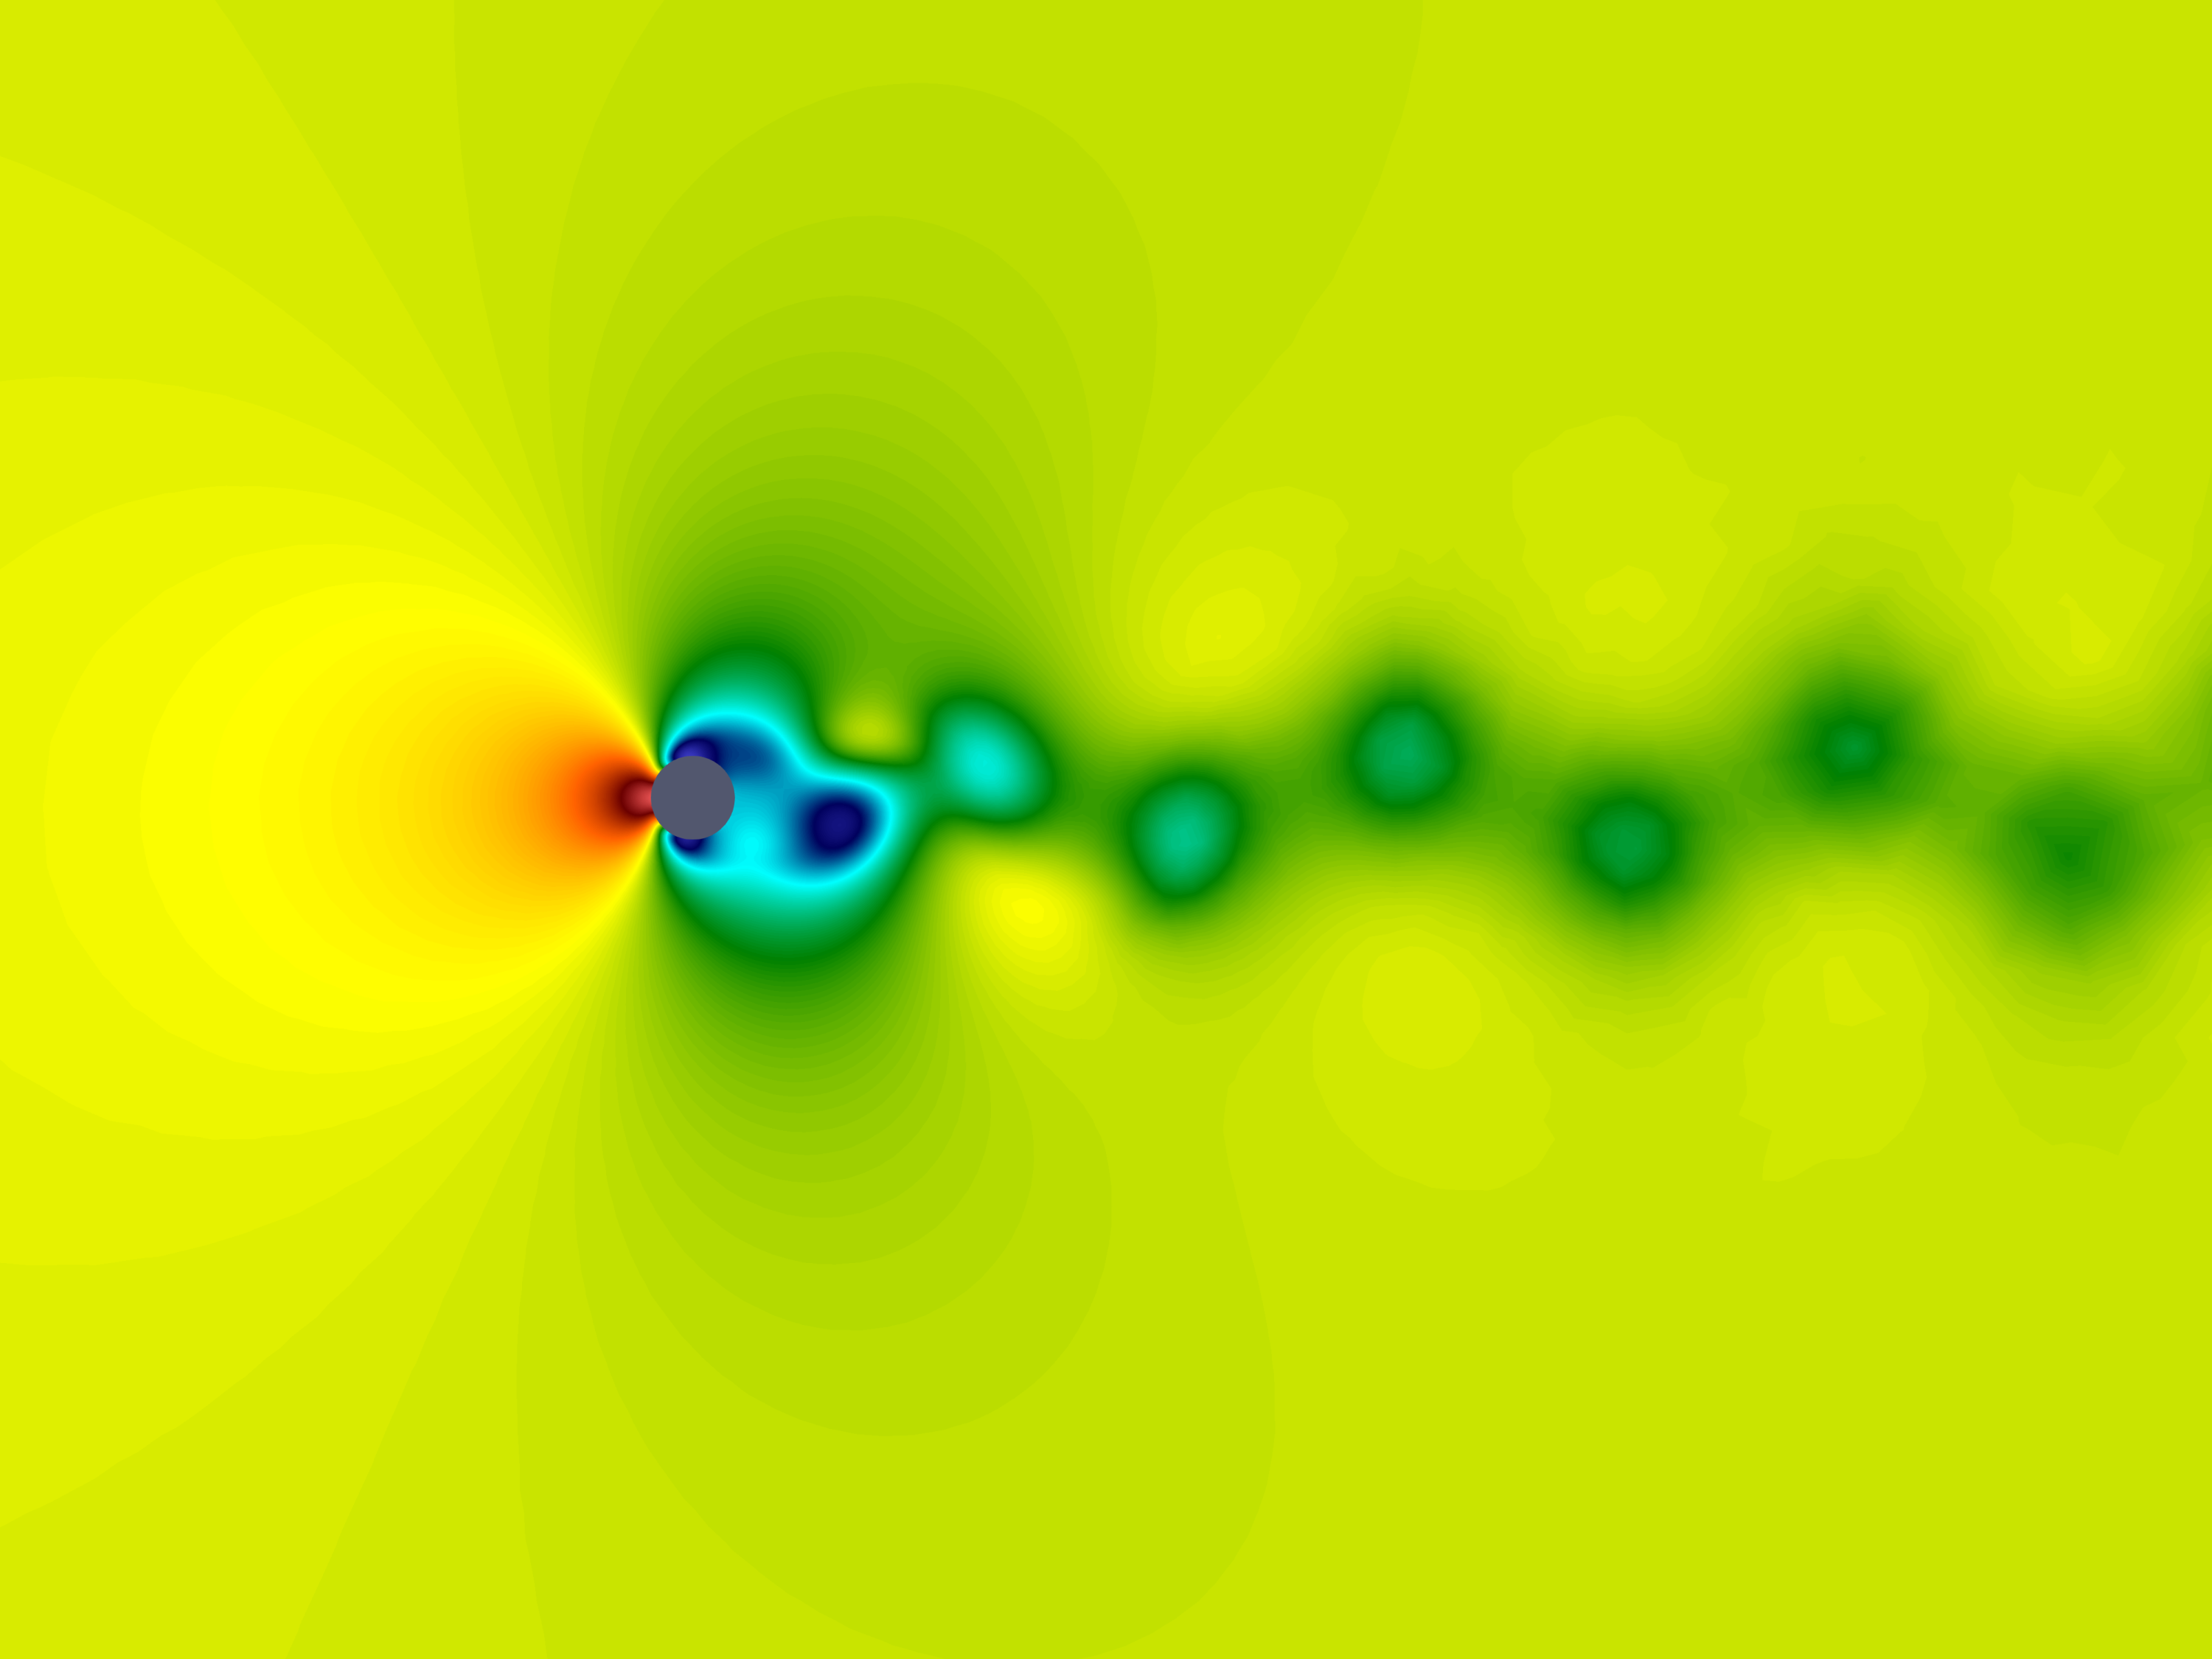
\includegraphics[scale=0.15,trim=5cm 5cm 5cm 6cm, clip=true]{Imagens/Cap2/cilindro_press2050.pdf}} \\
	\subfloat[$nT + n2T/3$]{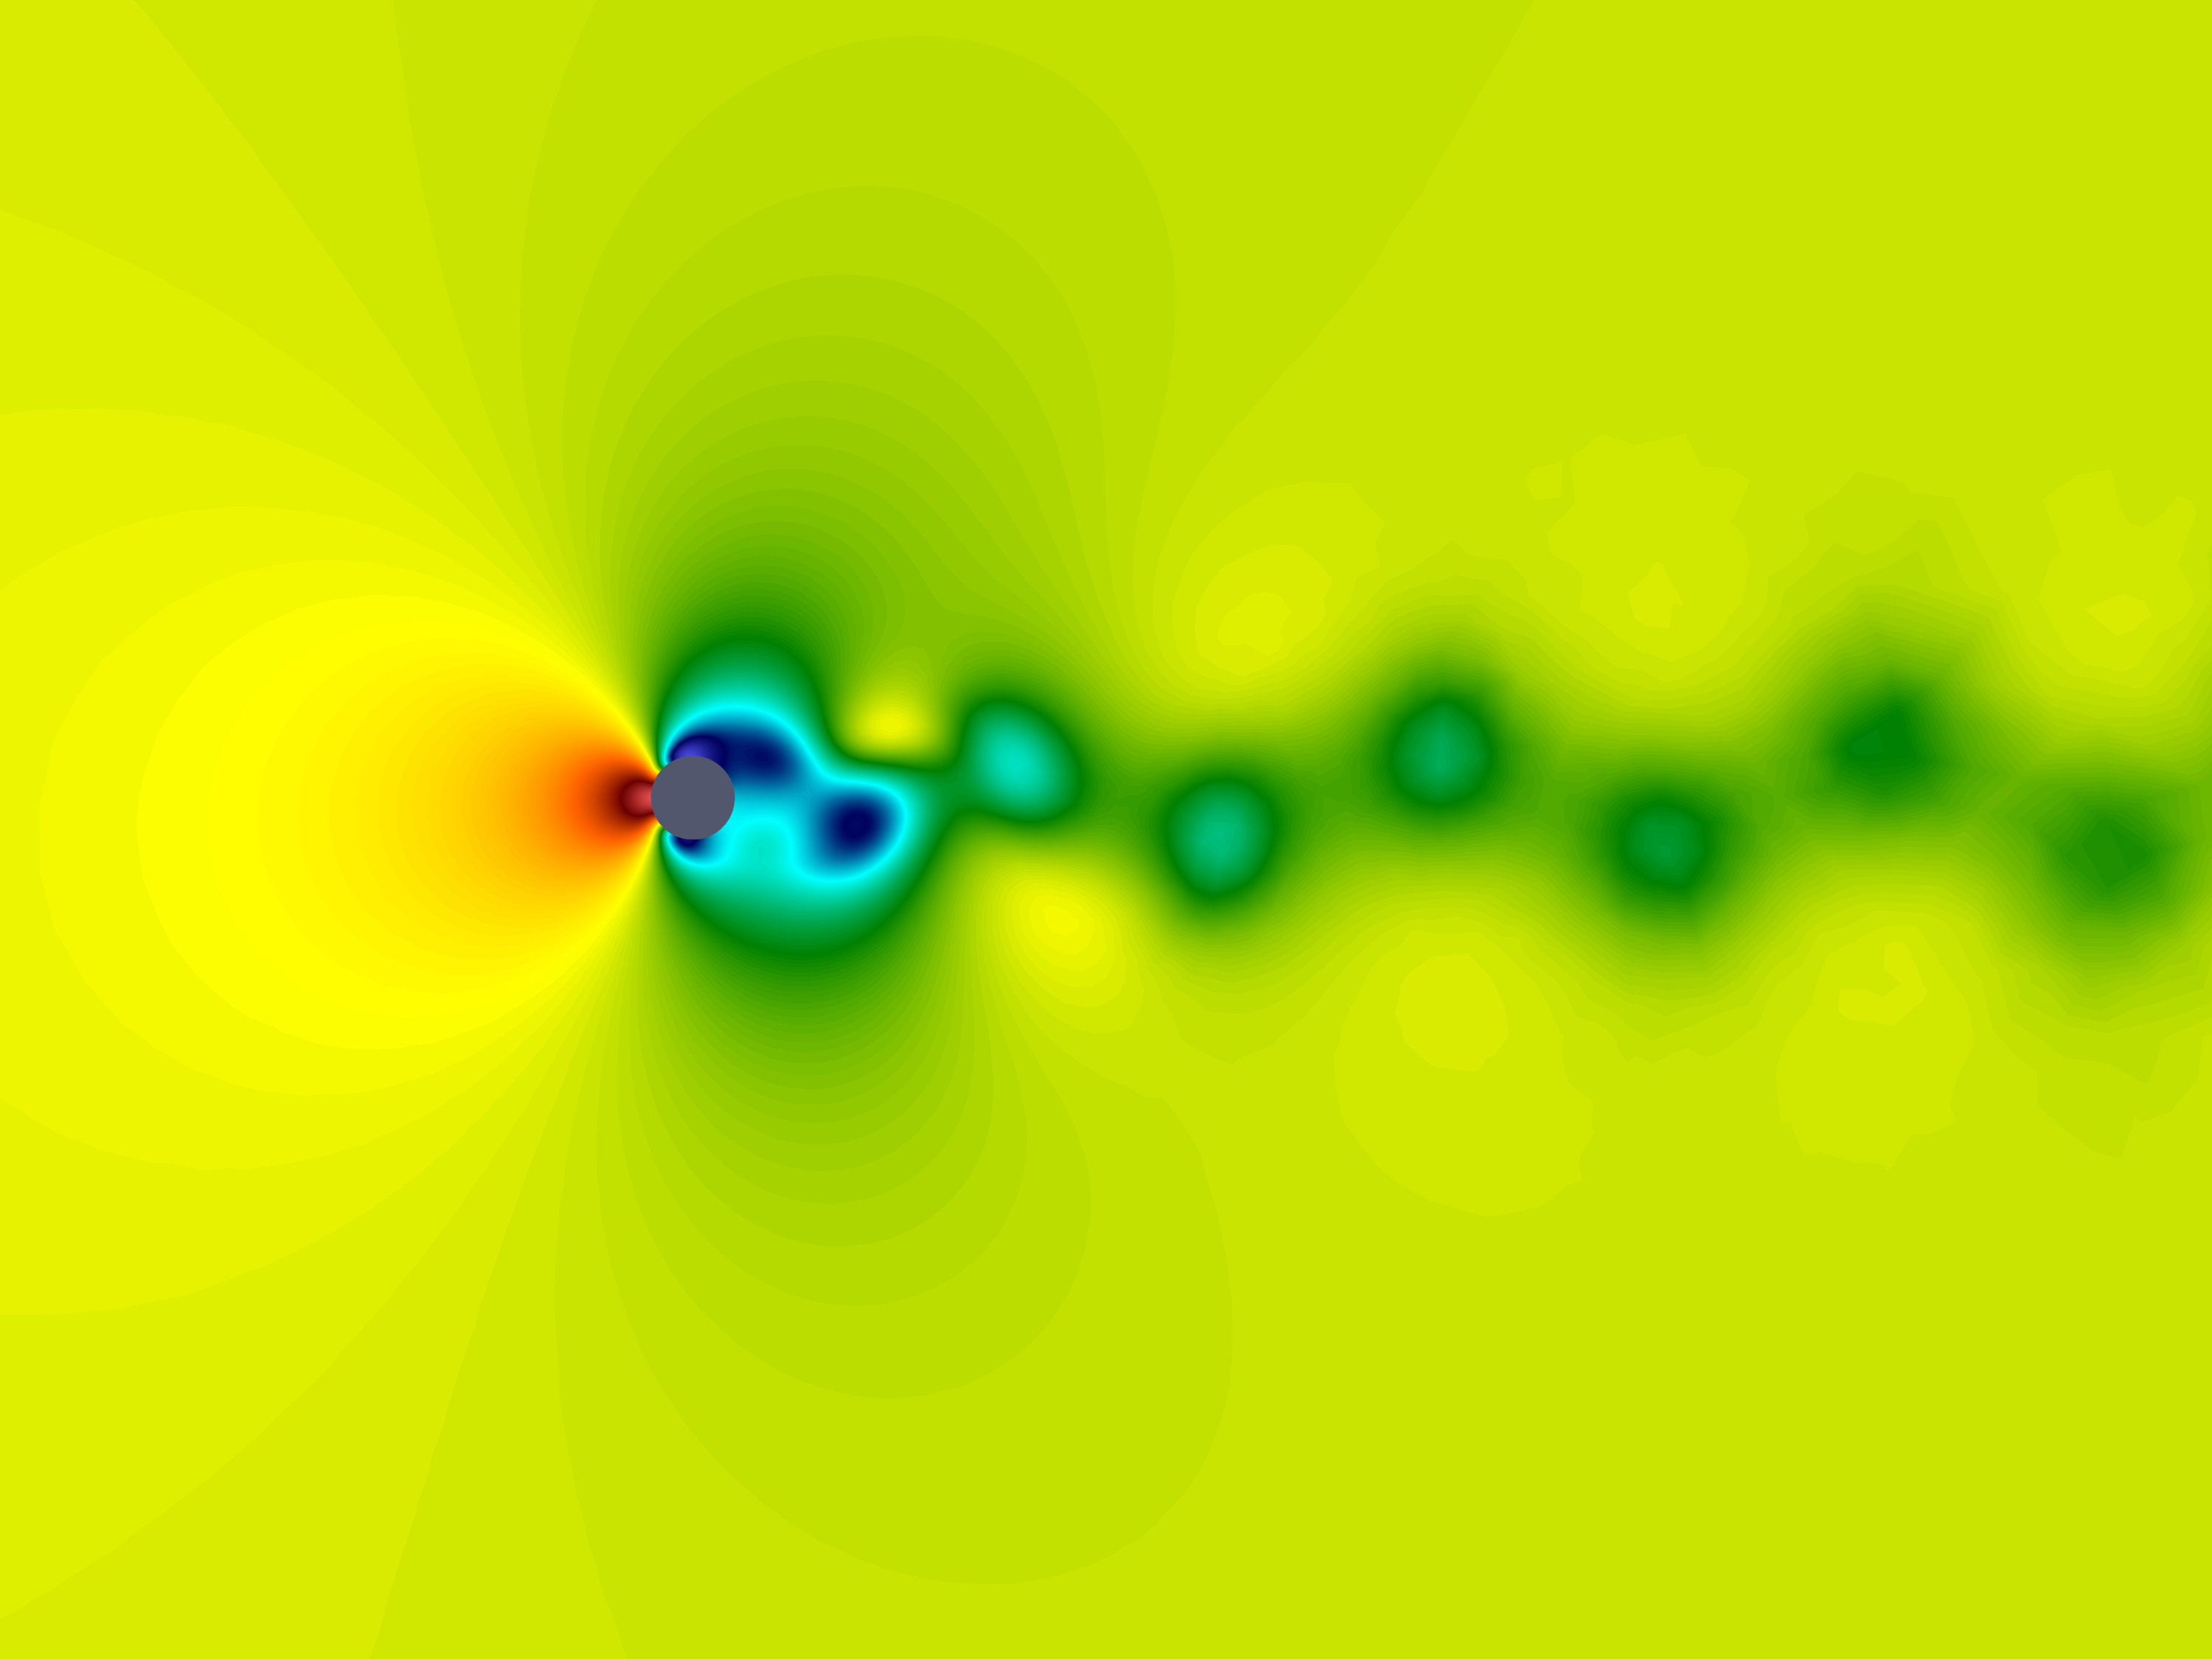
\includegraphics[scale=0.15,trim=5cm 5cm 5cm 6cm, clip=true]{Imagens/Cap2/cilindro_press2060.pdf}} \
	\subfloat[$nT + n5T/6$]{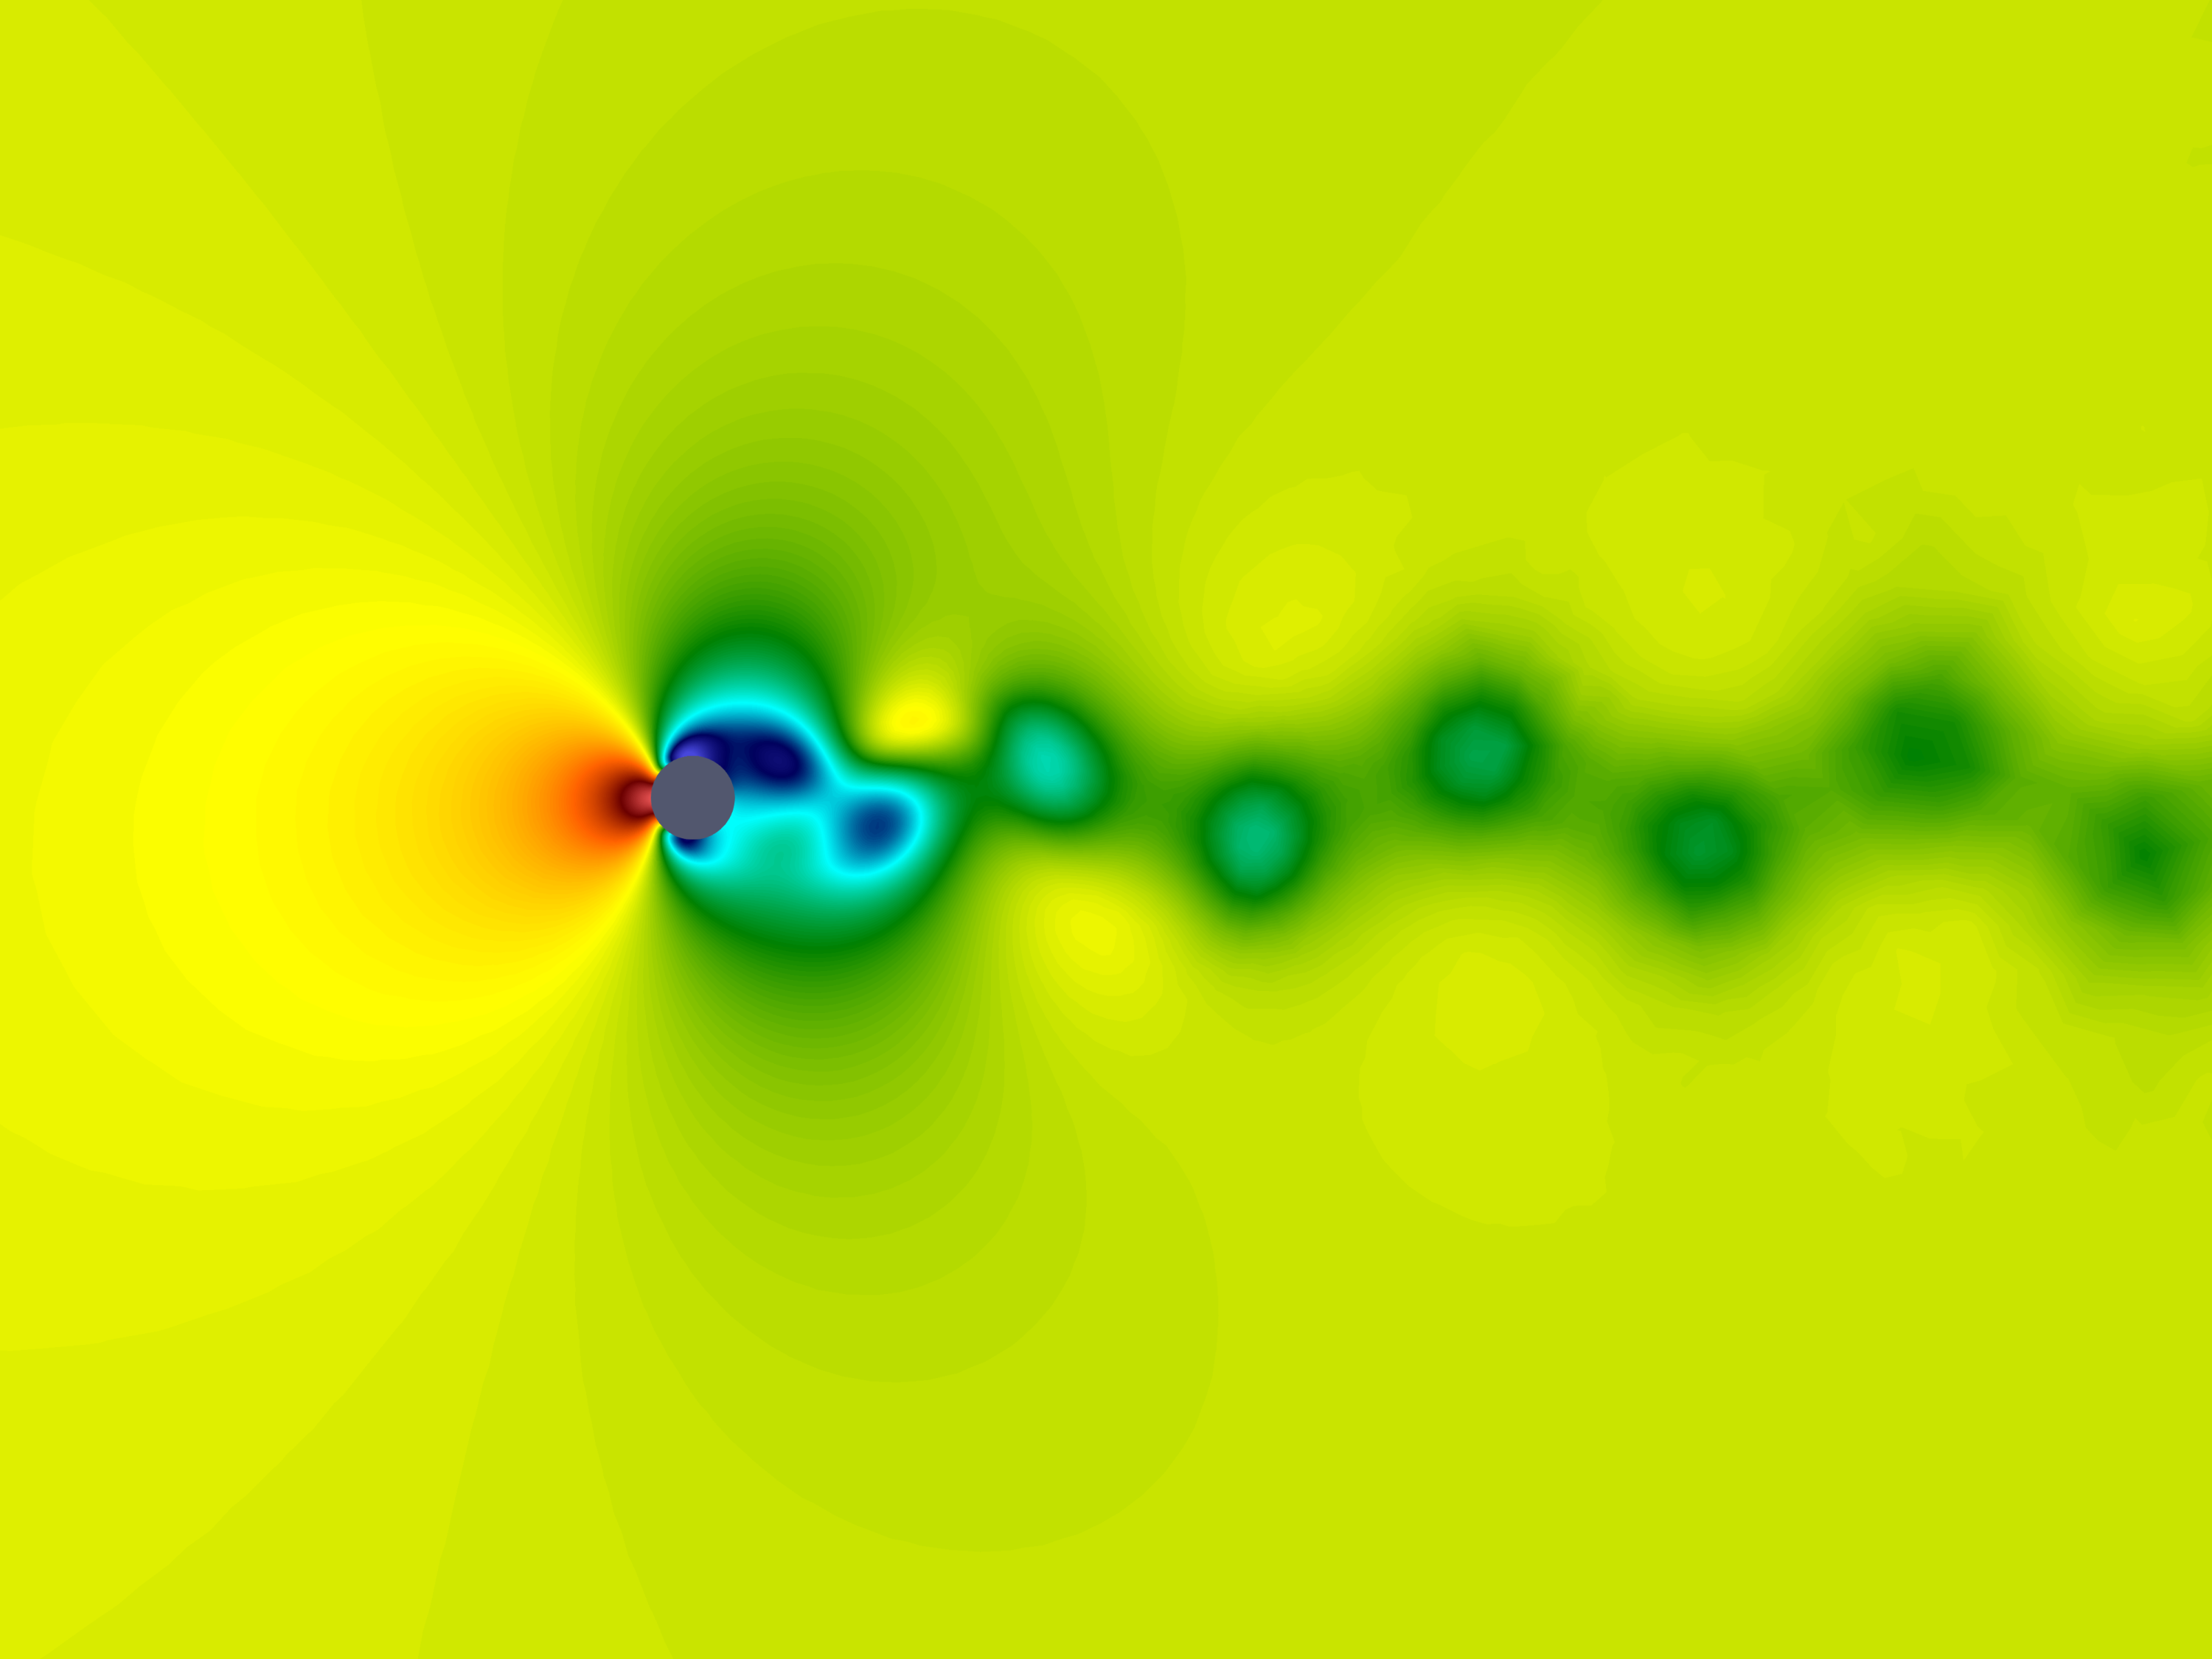
\includegraphics[scale=0.15,trim=5cm 5cm 5cm 6cm, clip=true]{Imagens/Cap2/cilindro_press2070.pdf}} \\
	{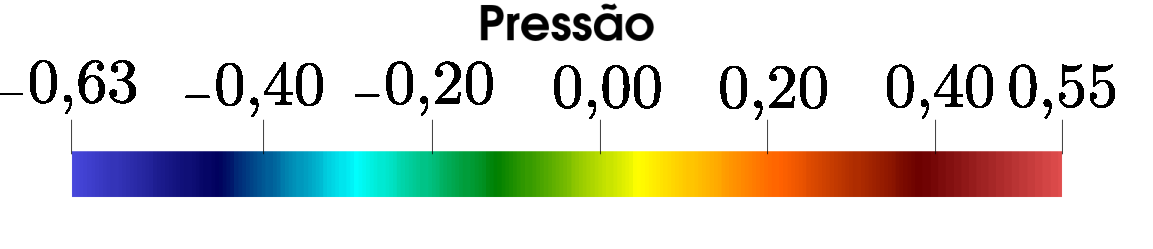
\includegraphics[trim=0cm 0.2cm 0cm 0cm,clip=true,scale=0.3]{Imagens/Cap2/cilindro_legendaPress.pdf}}
	\label{fig:cilindro_camposPressao}
	\legend{Fonte: Elaborada pela autora}
\end{figure}

\subsection{Escoamento sobre cavidade com discretização 3D} \label{capitulo:Cap2:VerApl:CavQuad}

Este exemplo considera uma cavidade hexaédrica com velocidade prescrita horizontal $u_{\infty}$ prescrita em sua face superior. A geometria do problema bem como as condições de contorno são apresentadas na Figura \ref{fig:cavidade_geometria}. As paredes da cavidade são rígidas, com paredes laterais e do fundo com condição de aderência, e adicionalmente, condição de simetria na direção $y_3$. A cavidade possui na direção $y_3$ uma espessura de $0,03$. A discretização espacial em elementos finitos utilizada é apresentada na Figura \ref{fig:cavidade_malha}, a qual consiste em 7252 elementos tetraédricos quadráticos e 14727 nós.  Embora este problema possa ser representado por uma discretização bidimensional, adota-se uma discretização 3D para um primeiro teste das implementações dos elementos finitos tetraédricos.

\begin{figure}[H]
	\caption{Cavidade quadrada: Geometria, condições de contorno e malha de elementos finitos}
	\centering
	\subfloat[Geometria e condições de contorno\label{fig:cavidade_geometria}]{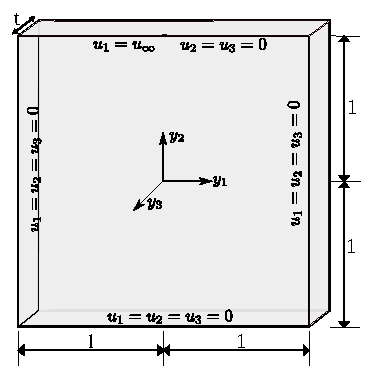
\includegraphics[scale=0.8,trim=0cm 0cm 0cm 0cm, clip=true]{Imagens/Cap2/cavidade_geometria.pdf}} \quad
	\subfloat[Discretização espacial.\label{fig:cavidade_malha}]{\includegraphics[trim=0 0 0 0,clip,scale=0.15]{Imagens/Cap2/cavidade_malha.png}}
	\legend{Fonte: Elaborada pela autora}
\end{figure}


O problema é estudado para 3 diferentes números de Reynolds (100, 400 e 1000), calculados de acordo com Equação \eqref{eq:Reynolds}, considerando $L$ como sendo o comprimento do lado da cavidade. O problema foi simulado para uma velocidade na parede superior de $u_{\infty} = 1,0$, $\density = 1,0$, $\timeStep = 0,05$, e $\specRadius = 0$, sendo a viscosidade do fluido variada de modo a alterar o número de Reynolds. A simulação foi mantida até que se atingiu o estado estacionário de escoamento. 

Os perfis de velocidade adimensionalizada ($\velocity/\velocinfty$) ao longo de duas linhas centrais nas direções $y_1$ e $y_2$ posicionadas no centro da espessura da direção $y_3$, são apresentados na Figura \ref{fig:cavidade_graficos} e comparados com a referência de \citeonline{GhiaGS:1982}.

\begin{figure}[!htbp]
	\caption{Cavidade quadrada: Perfis de velocidade adimensionalizados nas direções $y_1$ e $y_2$  }
	\centering
	\subfloat[\label{fig:cavidade_Re100}$Re$=100]{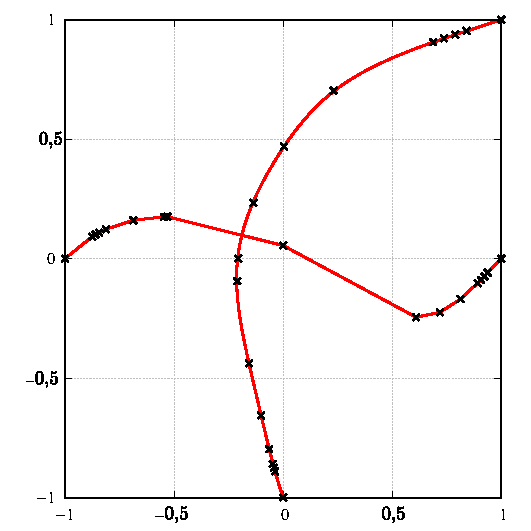
\includegraphics[scale=0.6,trim=0.55cm 0cm 0.3cm 0.2cm, clip=true]{Imagens/Cap2/cavidade_Re100.pdf}} \subfloat[\label{fig:cavidade_Re400}$Re$=400]{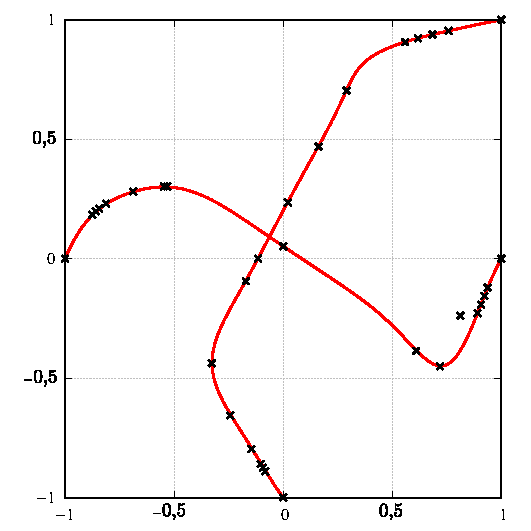
\includegraphics[scale=0.6,trim=0.55cm 0cm 0.3cm 0.2cm, clip=true]{Imagens/Cap2/cavidade_Re400.pdf}}\\ 
	\subfloat[\label{fig:cavidade_Re1000}$Re$=1000]{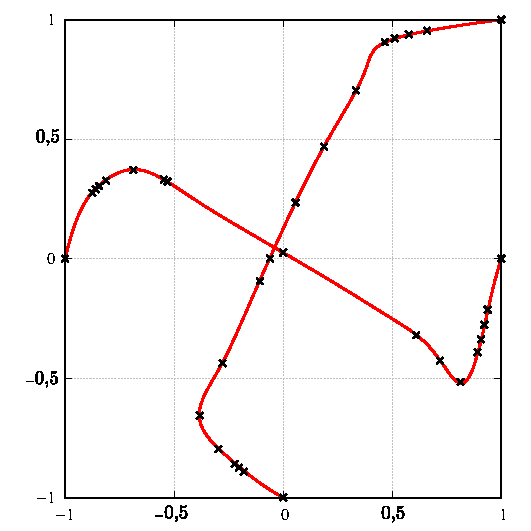
\includegraphics[scale=0.6,trim=0.55cm 0cm 0.3cm 0.2cm, clip=true]{Imagens/Cap2/cavidade_Re1000.pdf}} \ 
	\subfloat{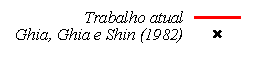
\includegraphics[scale=1.]{Imagens/Cap2/cavidade_legenda.pdf}}
	\legend{Fonte: Elaborada pela autora}
	\label{fig:cavidade_graficos}
\end{figure}

Os campos de velocidade e de pressão para a situação estacionária são apresentados na Figura \ref{fig:cavidade_vel} e Figura \ref{fig:cavidade_press}, respectivamente. Ressalta-se que para a simulação, por se tratar de um problema com todos os contornos com condição de Dirichlet impostos, a pressão torna-se indefinida. Por esse motivo, prescreveu-se pressão $\press = \press_{ref} =  0,0$ no canto superior direito da cavidade. 

\begin{figure}[!htbp]
	\caption{Cavidade quadrada: Campos de velocidade -  plano $y_1$$y_2$}
	\centering
	\setlength{\lineskip}{-10pt}
	\subfloat[\label{fig:cavidade_vel_Re100}$Re$=100]{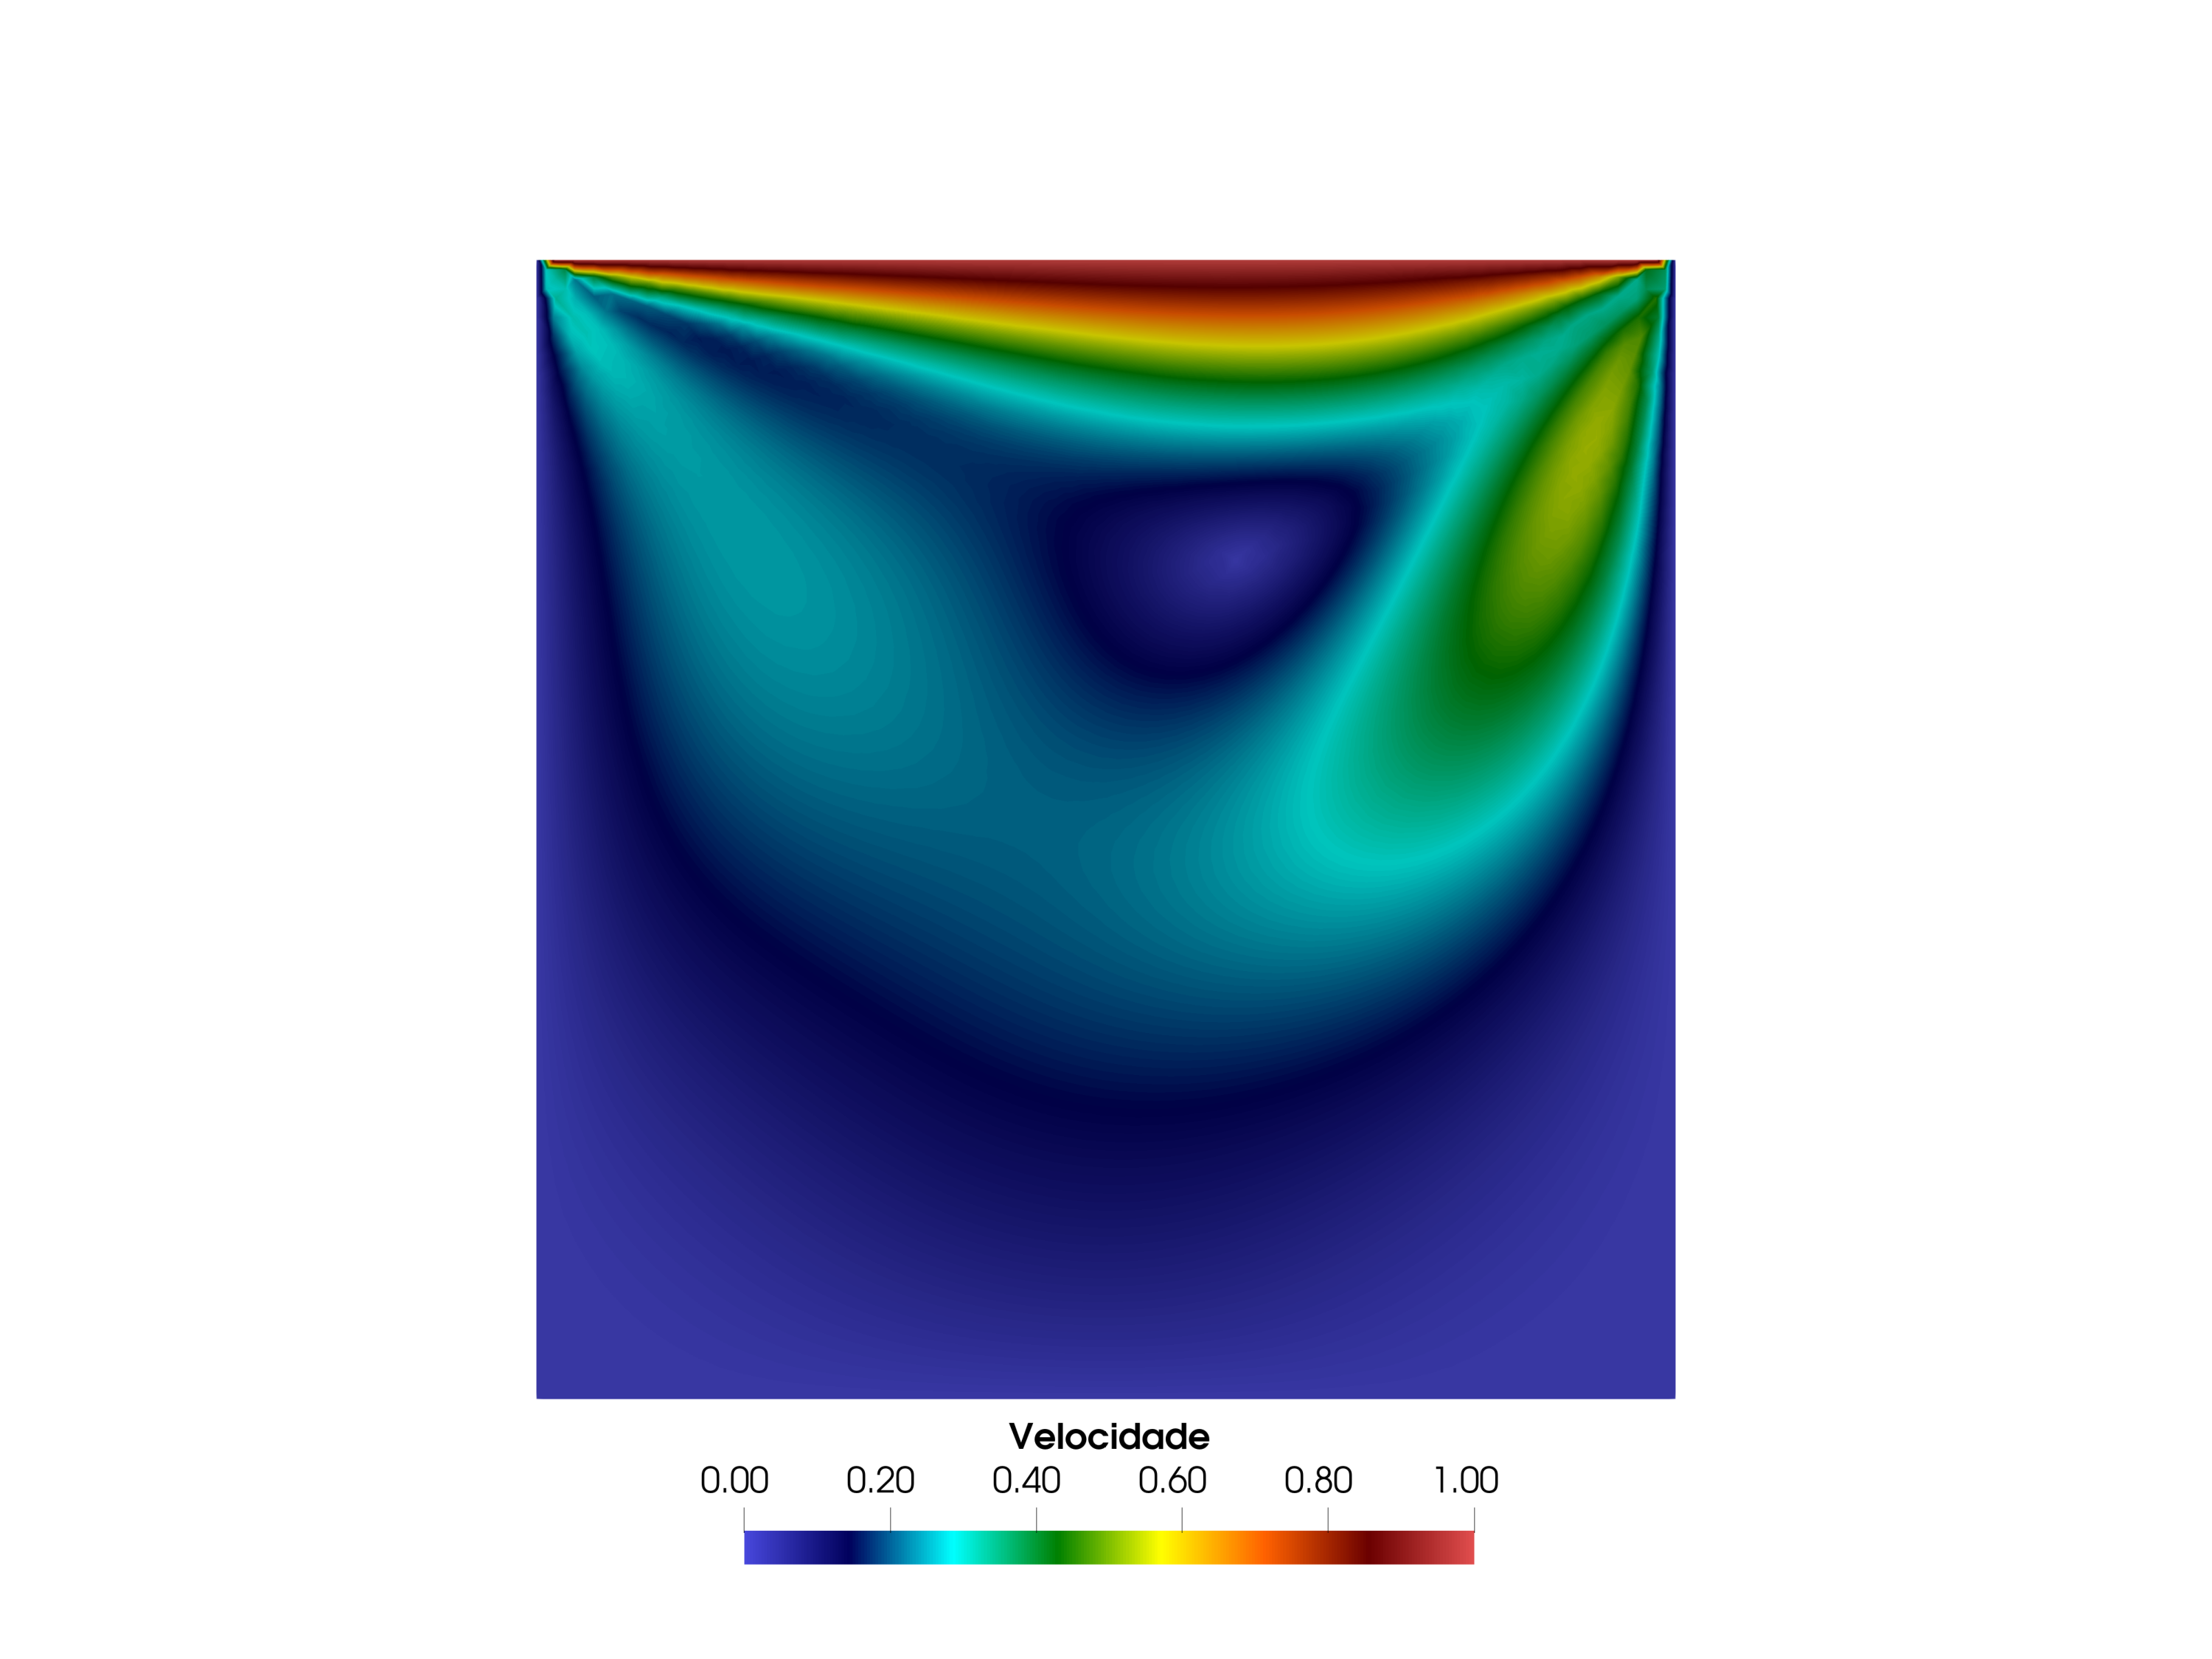
\includegraphics[scale=0.20,trim=12cm 5.5cm 12cm 5cm, clip=true]{Imagens/Cap2/cavidade_velRe100.pdf}} 
	\subfloat[\label{fig:cavidade_vel_Re400}$Re$=400]{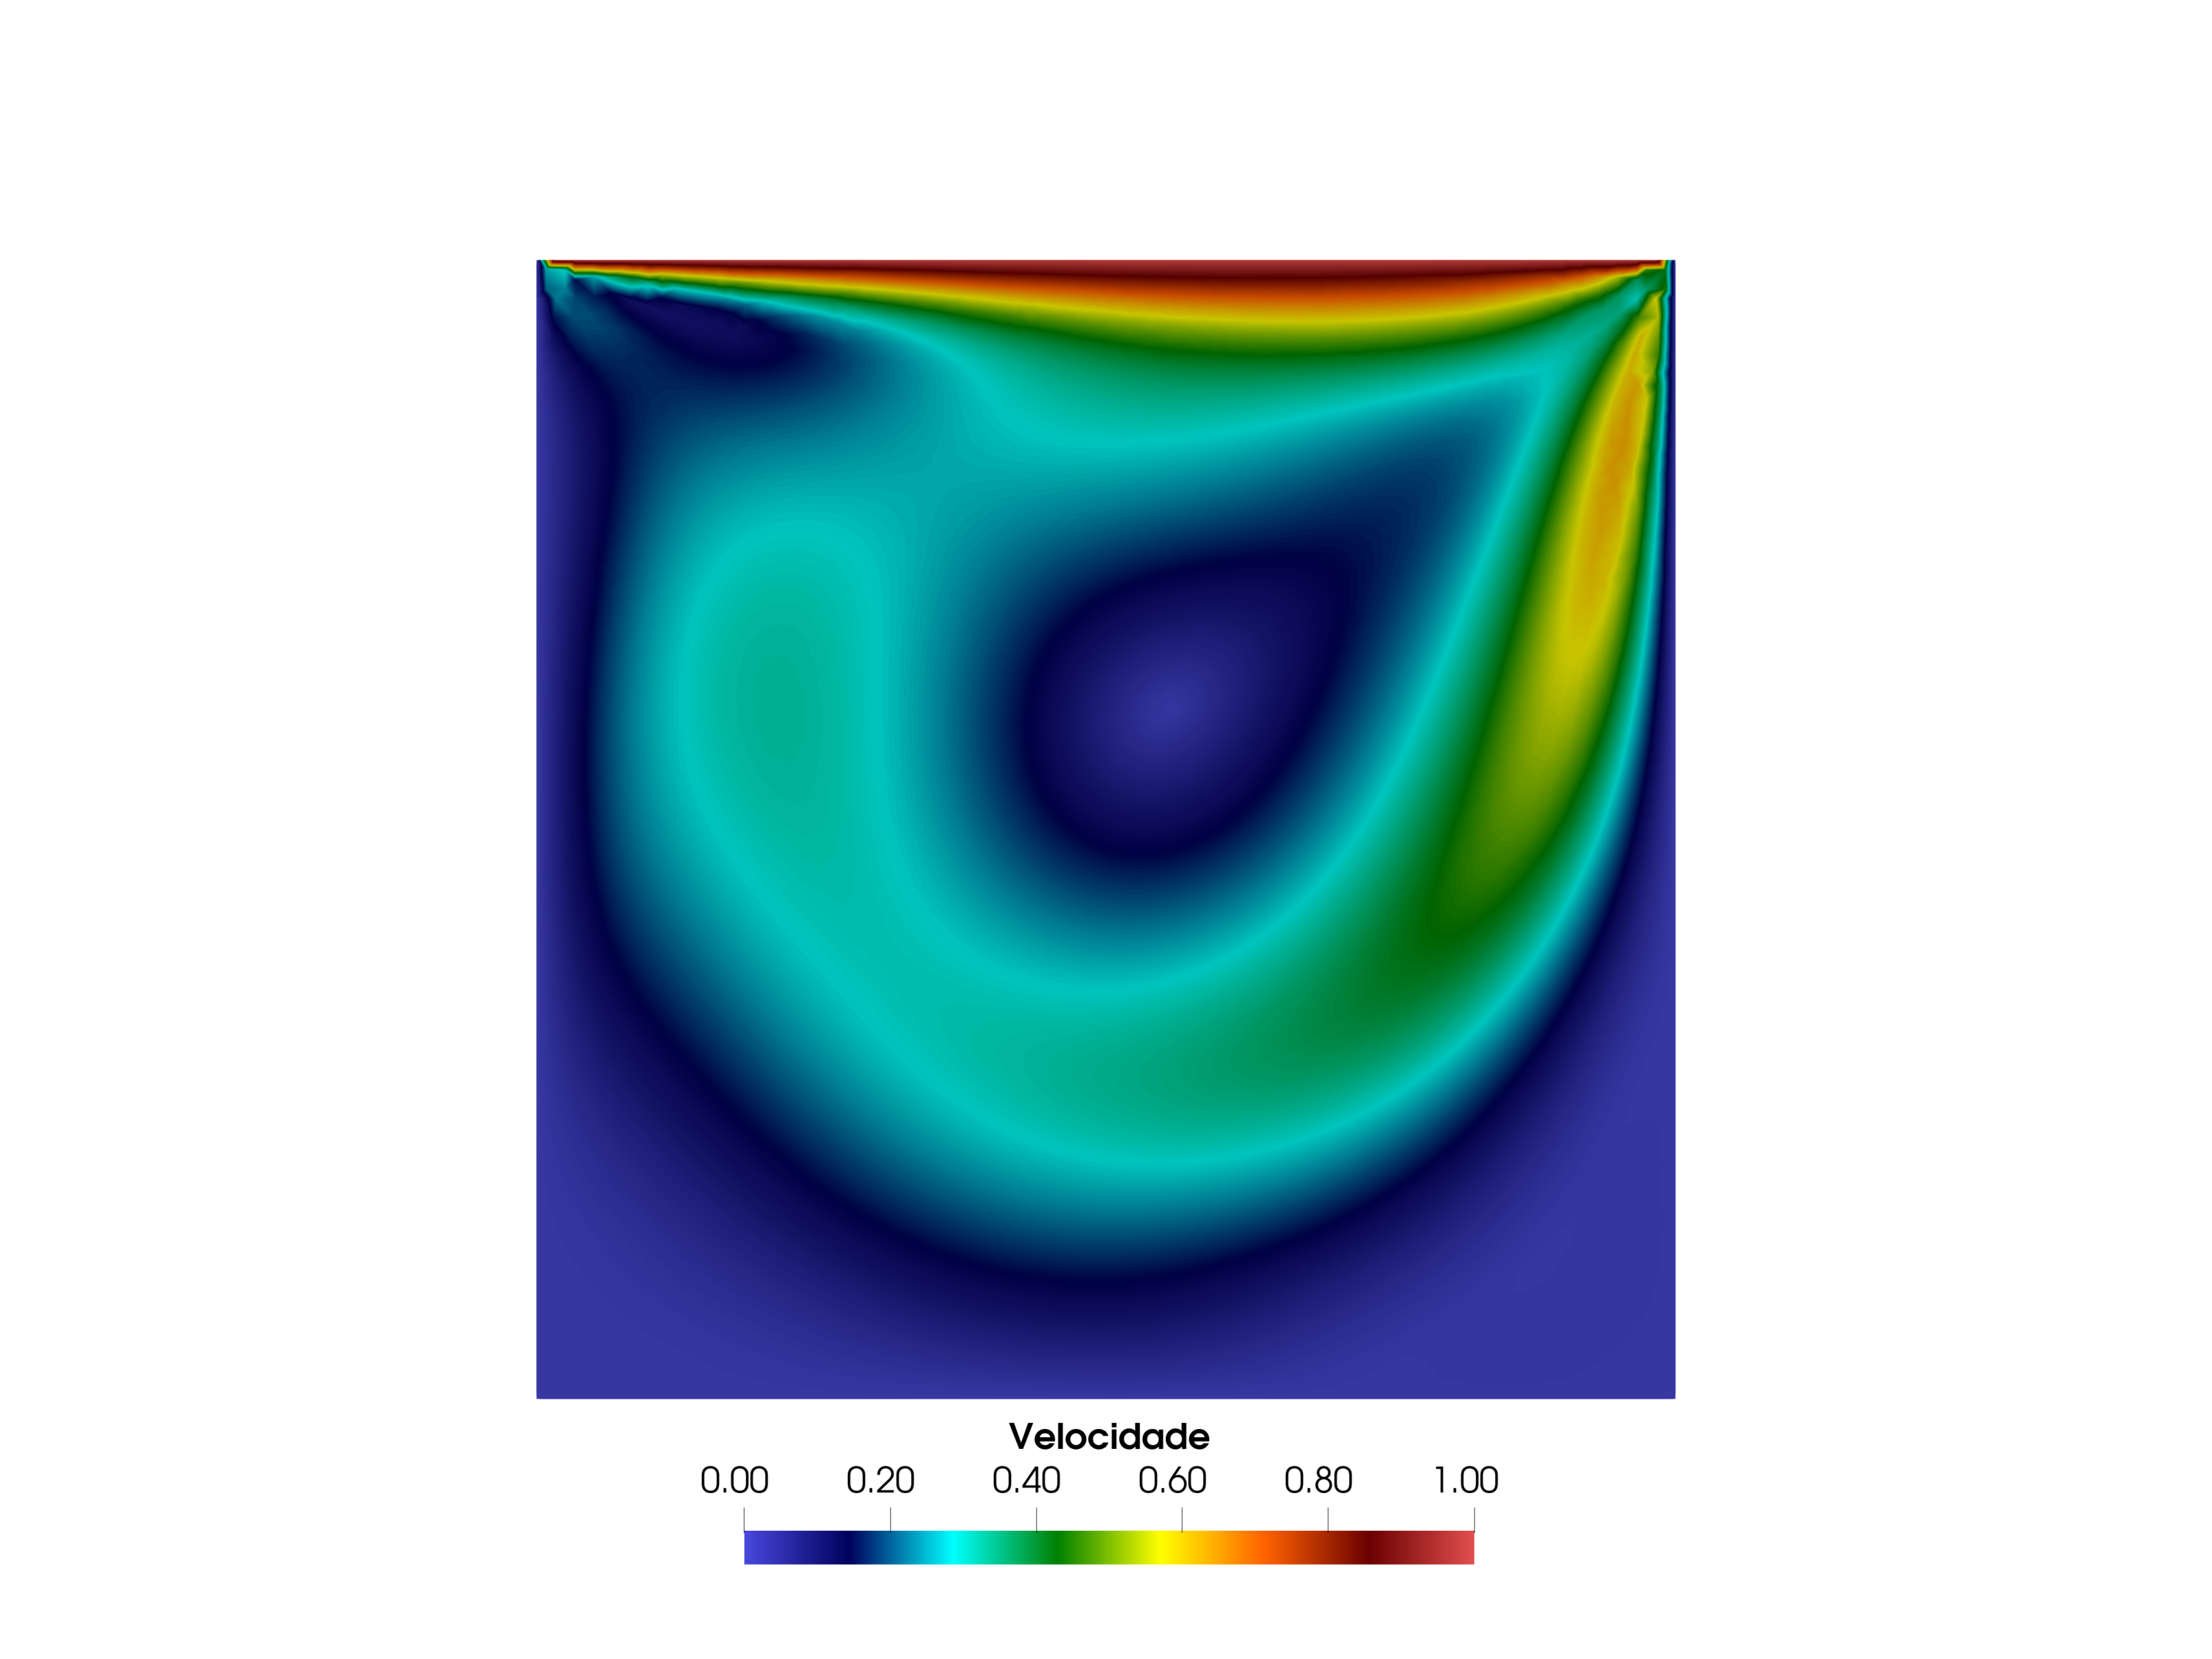
\includegraphics[scale=0.20,trim=12cm 5.5cm 12cm 5cm, clip=true]{Imagens/Cap2/cavidade_velRe400.pdf}}\\ 
	\subfloat[\label{fig:cavidade_vel_Re1000}$Re$=1000]{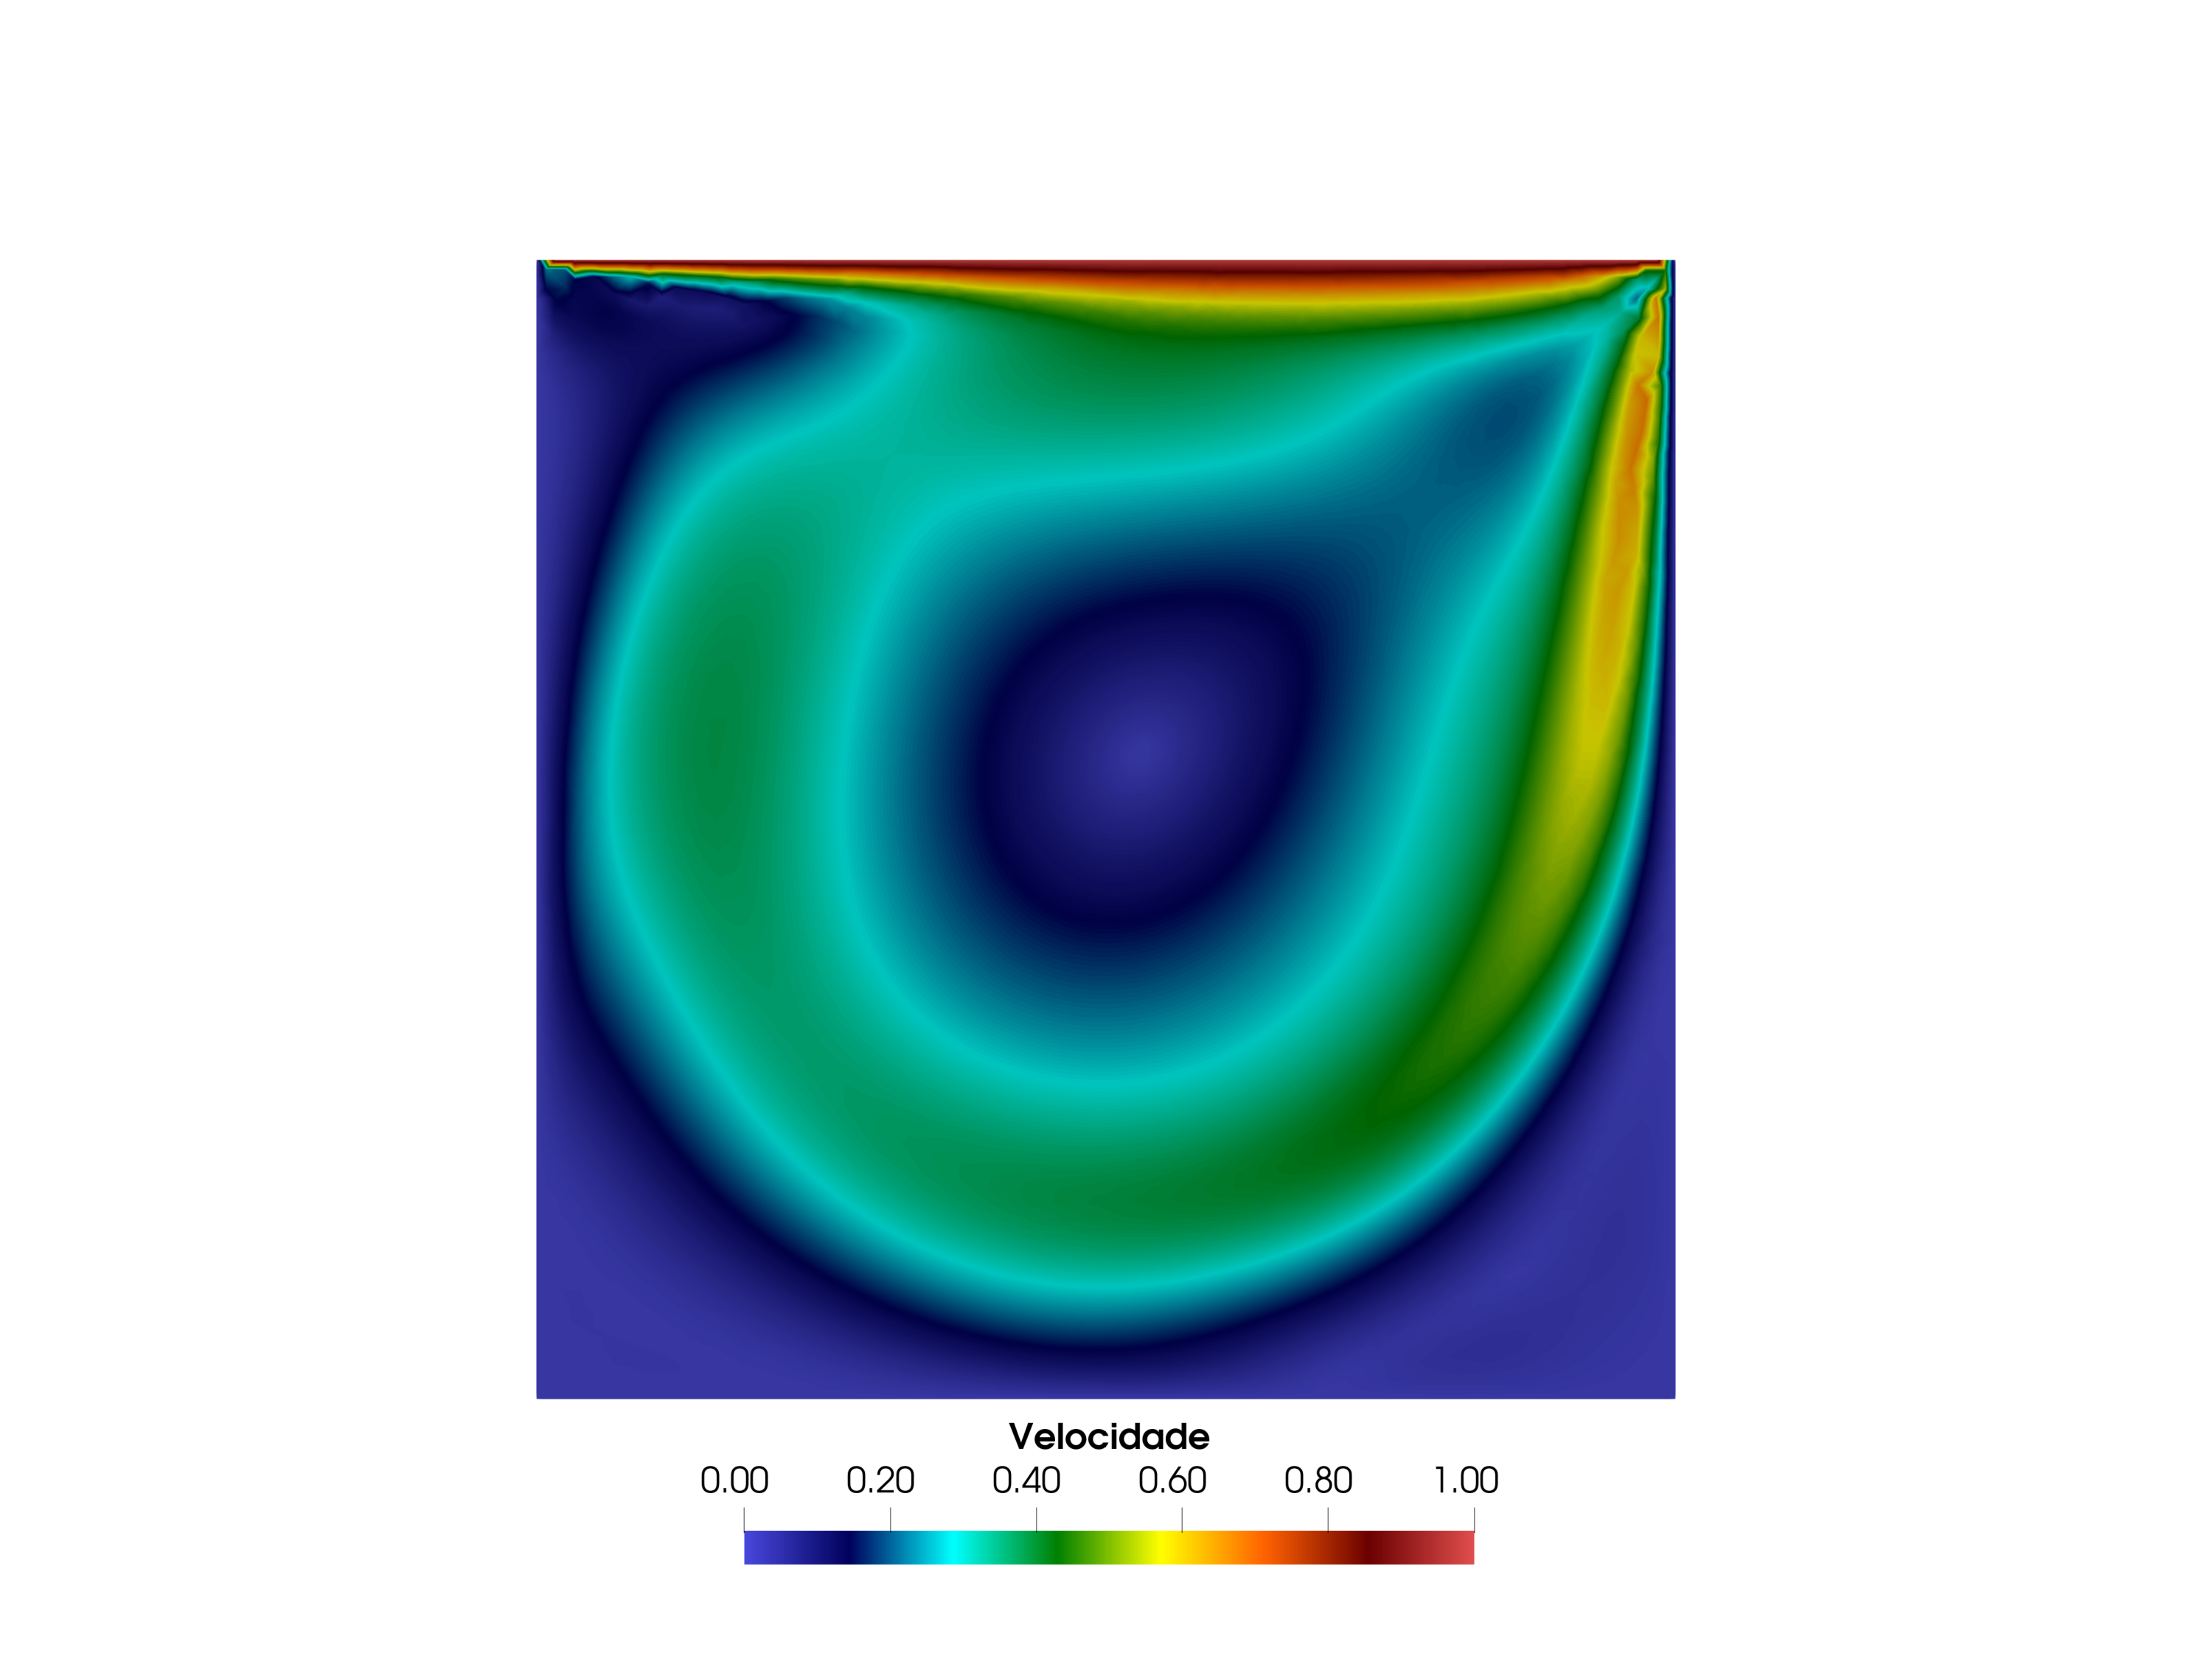
\includegraphics[scale=0.20,trim=12cm 5.5cm 12cm 5cm, clip=true]{Imagens/Cap2/cavidade_velRe1000.pdf}}\\[3.0ex]
	% Barra de cores (legenda) separada
	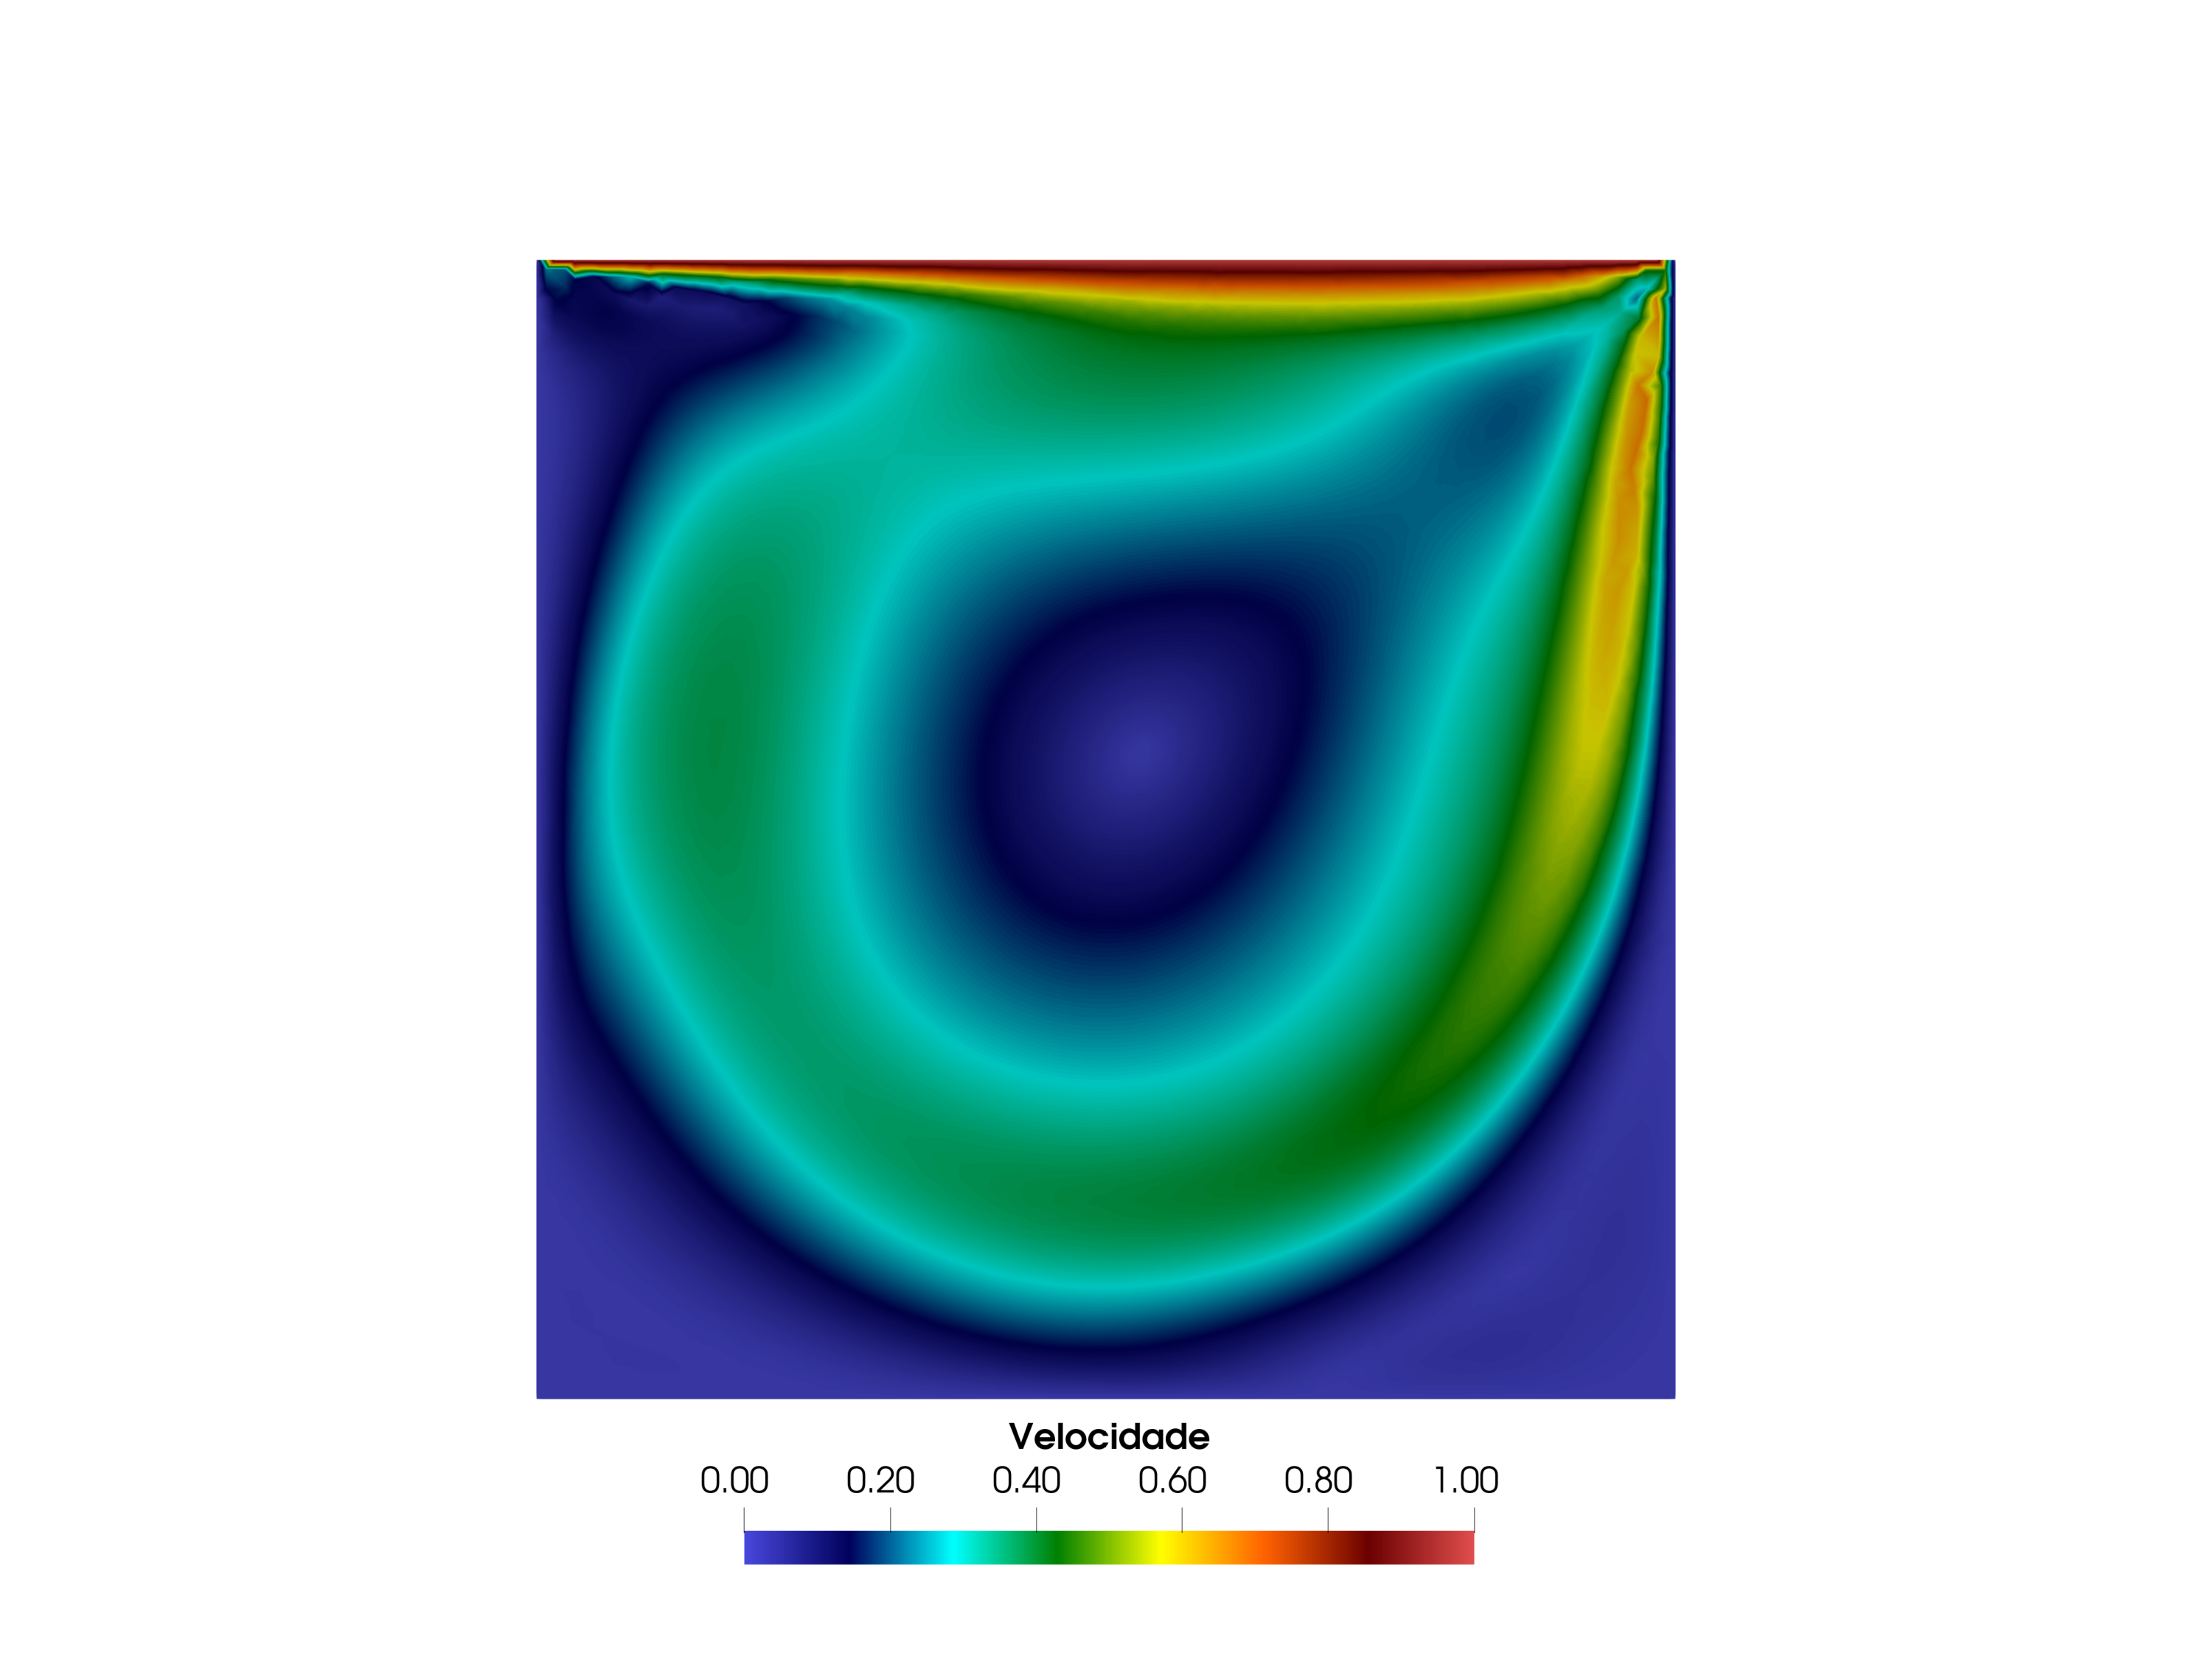
\includegraphics[scale=0.3,trim=12cm 2cm 12cm 32.5cm, clip=true]{Imagens/Cap2/cavidade_velRe1000.pdf}
	\legend{Fonte: Elaborada pela autora}
	\label{fig:cavidade_vel}
\end{figure}

\begin{figure}[!htbp]
	\caption{Cavidade quadrada: Campos de pressão - plano $y_1$$y_2$}
	\centering
	\subfloat[\label{fig:cavidade_press_Re100}$Re$=100]{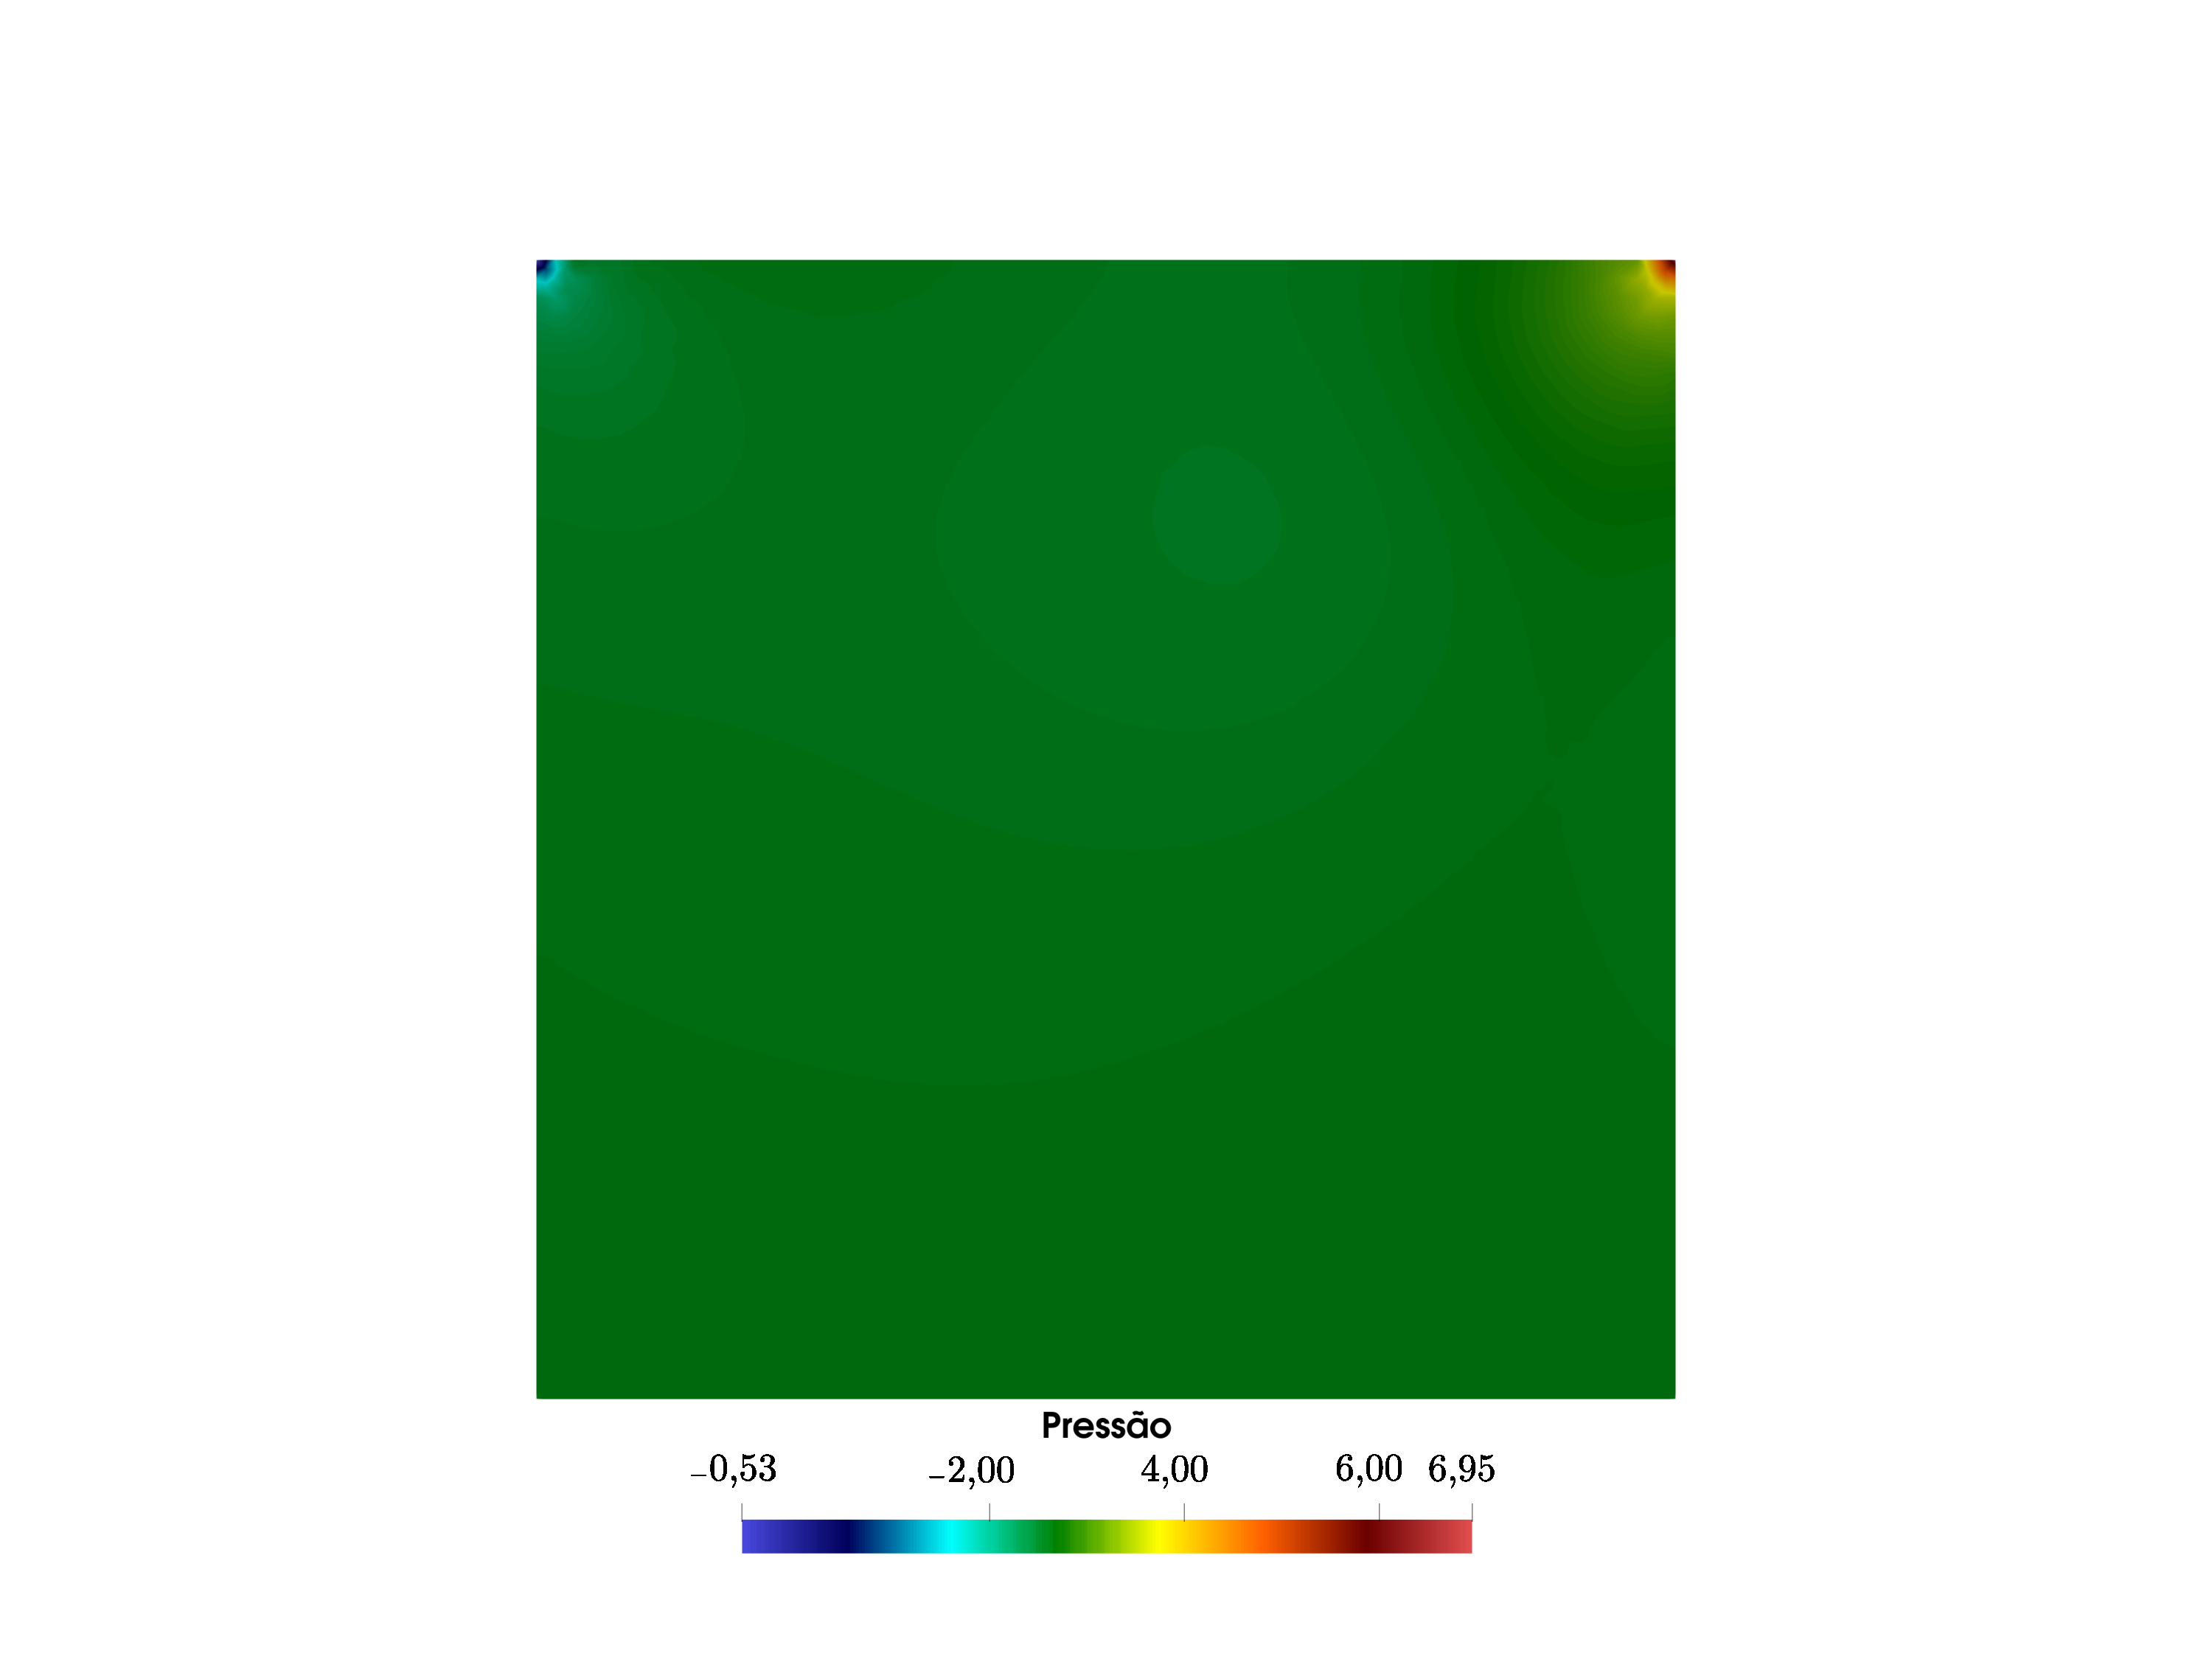
\includegraphics[scale=0.20,trim=12cm 2cm 12cm 5cm, clip=true]{Imagens/Cap2/cavidade_pressRe100.pdf}} 
	\subfloat[\label{fig:cavidade_press_Re400}$Re$=400]{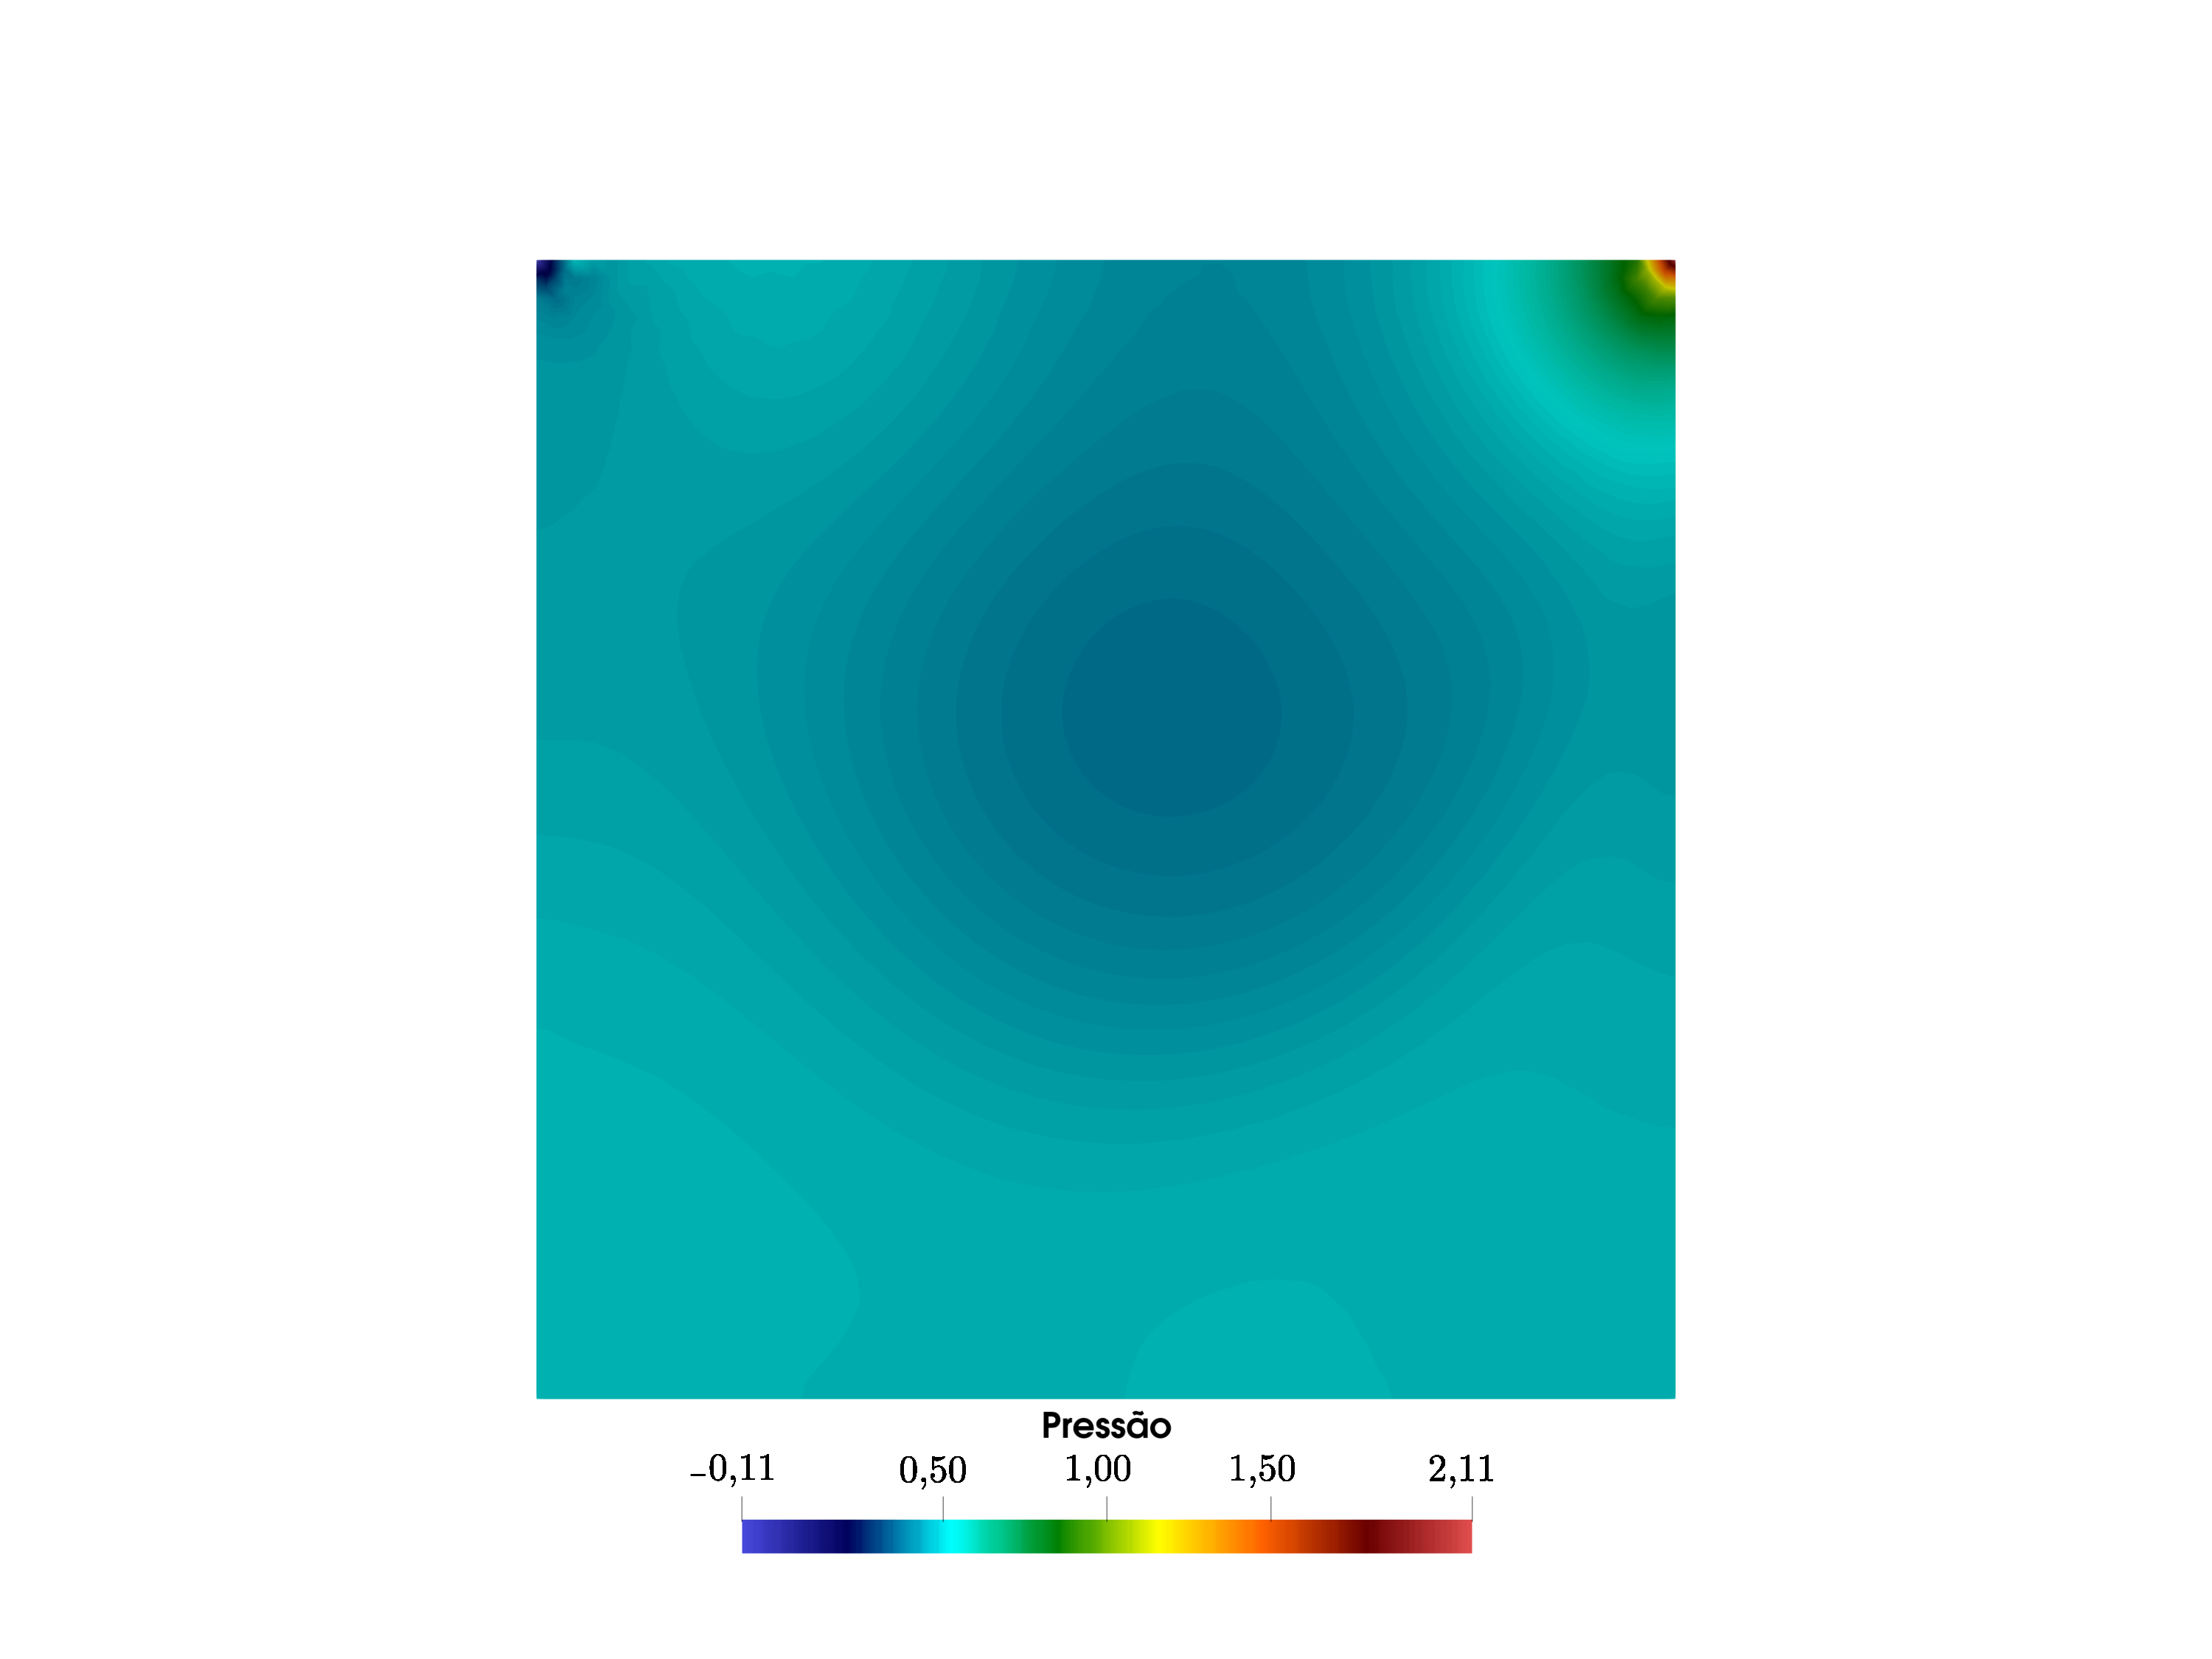
\includegraphics[scale=0.20,trim=12cm 2cm 12cm 5cm, clip=true]{Imagens/Cap2/cavidade_pressRe400.pdf}}\\ 
	\subfloat[\label{fig:cavidade_press_Re1000}$Re$=1000]{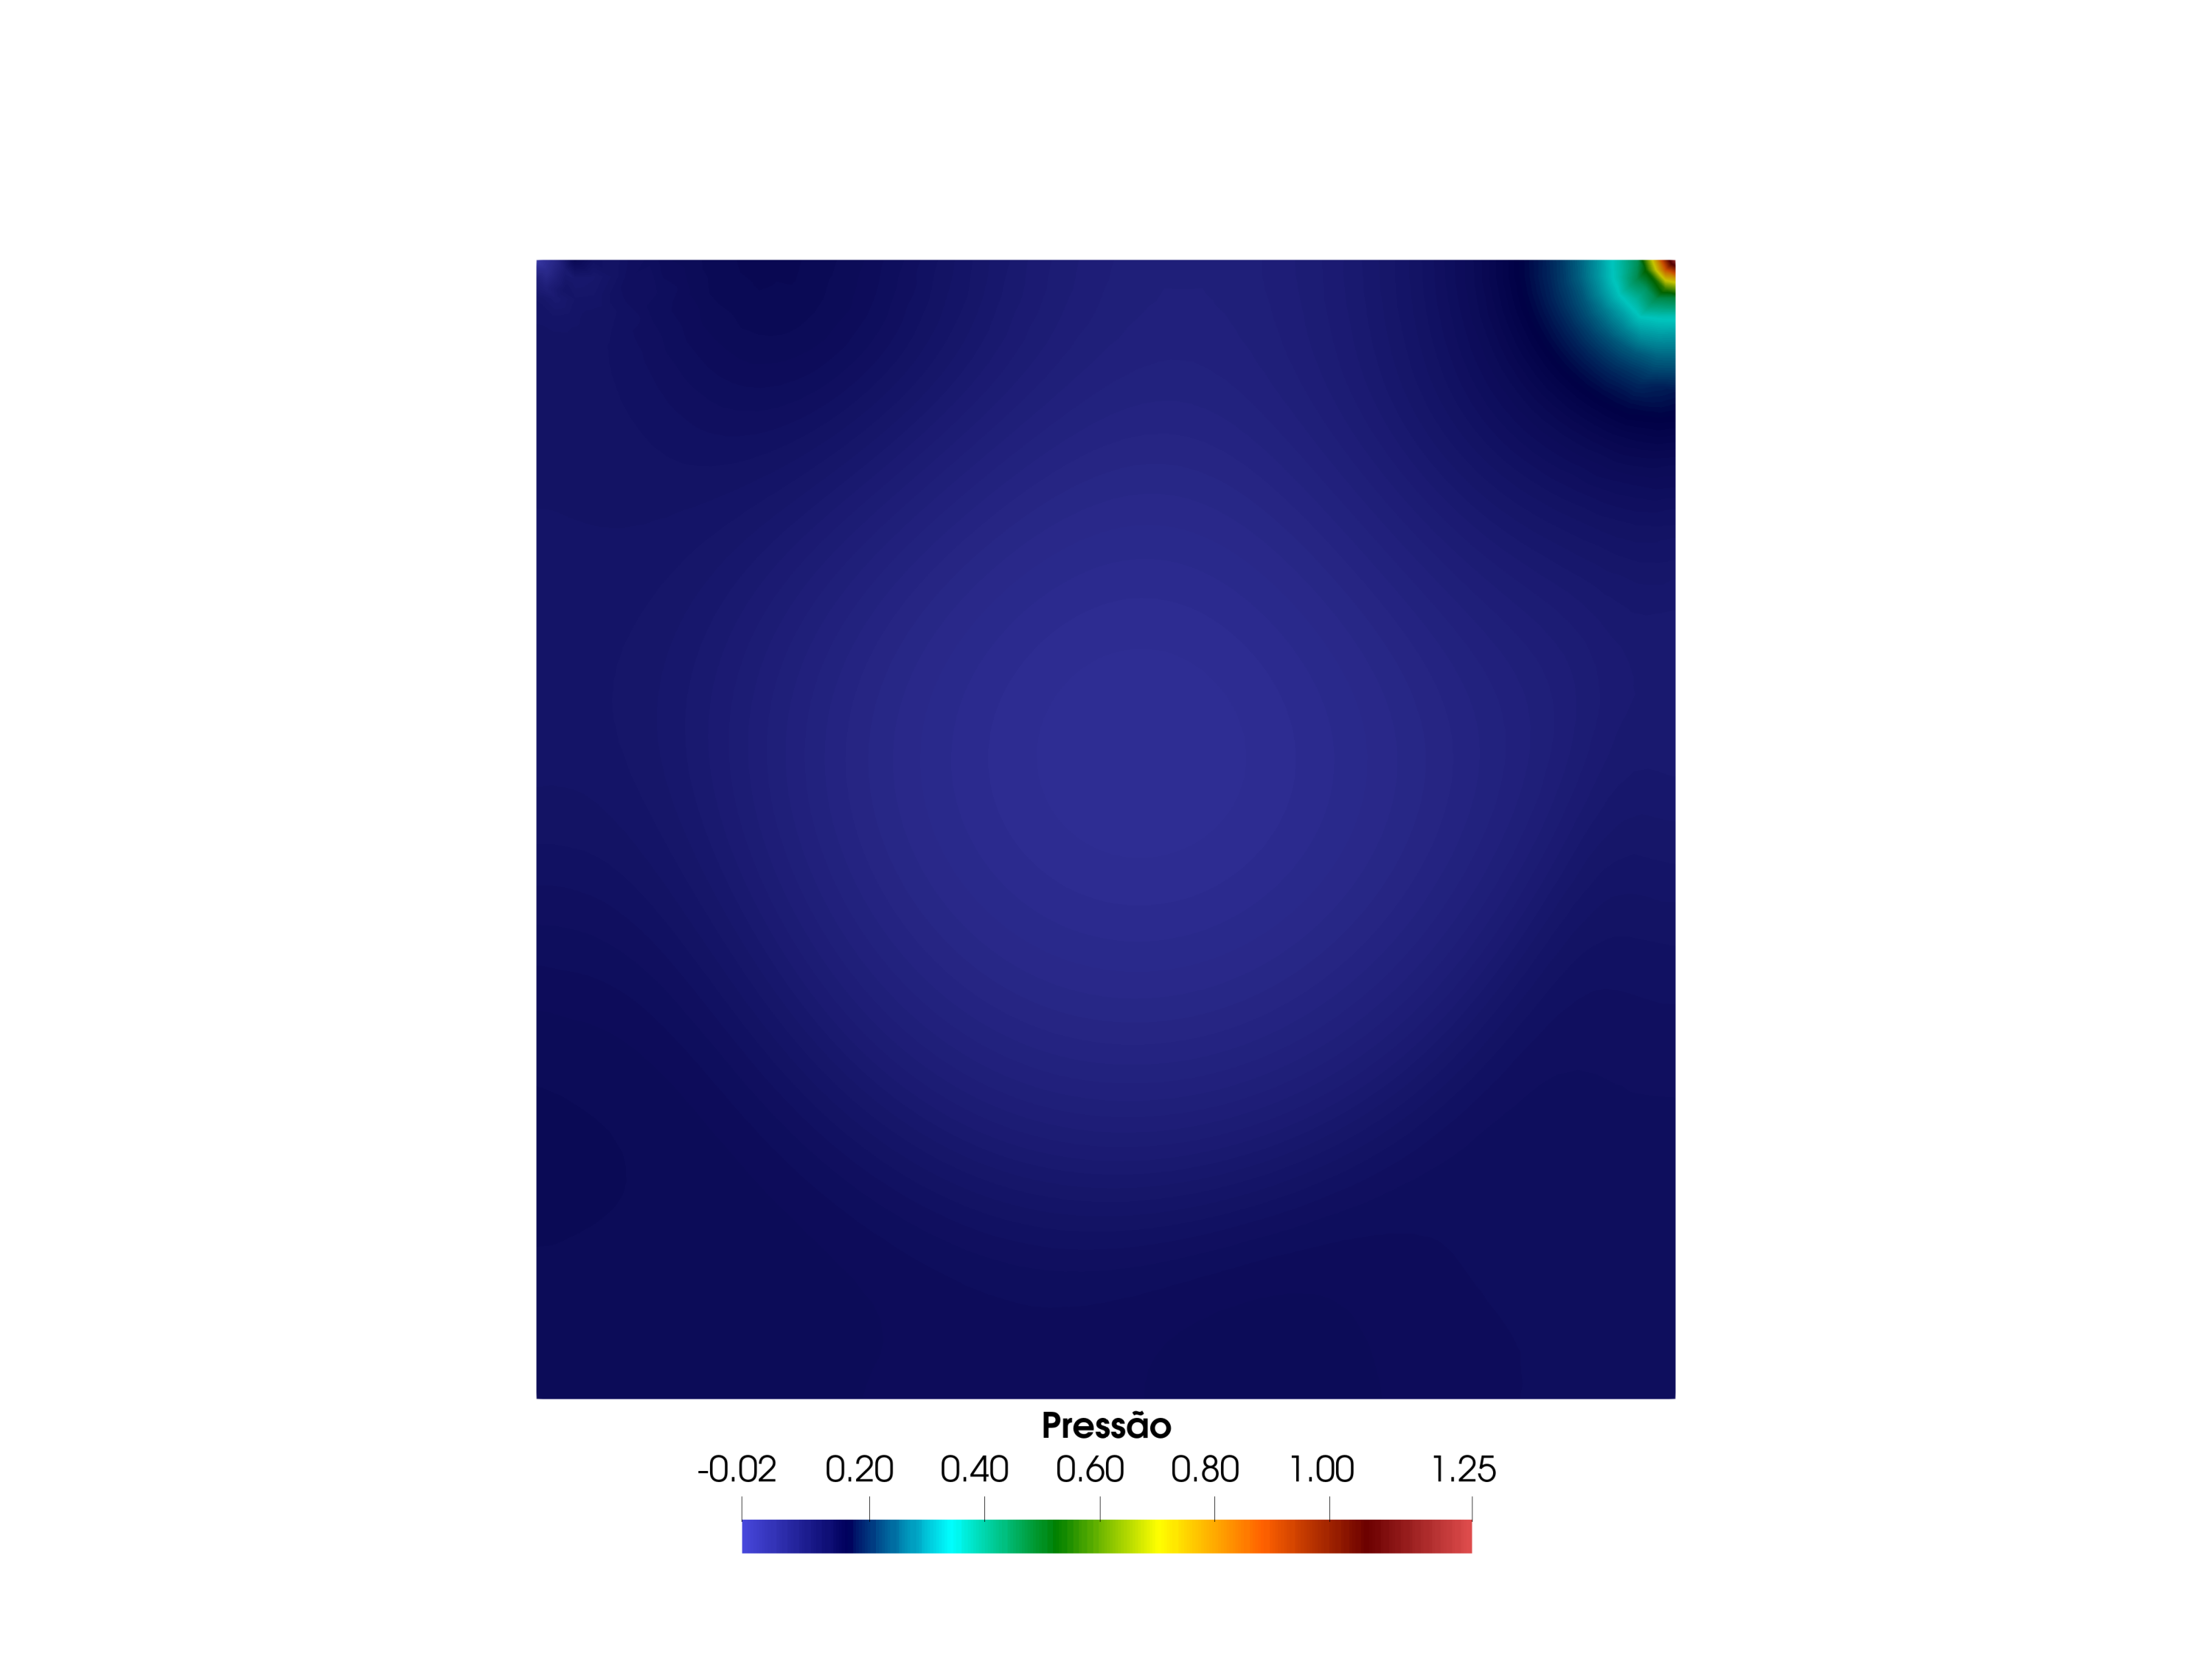
\includegraphics[scale=0.20,trim=12cm 2cm 12cm 5cm, clip=true]{Imagens/Cap2/cavidade_pressRe1000.pdf}}
	\legend{Fonte: Elaborada pela autora}
	\label{fig:cavidade_press}
\end{figure}
